\documentclass{book}

% Required for \includegraphics and \graphicspath
\usepackage{graphicx}

% Mathematical packages for symbols and equations
\usepackage{amsmath}
\usepackage{amssymb}
\usepackage{amsthm}

% For colored boxes and enhanced environments
\usepackage{tcolorbox}

% Add all possible image directories here
% The paths are relative to this file (book.tex)
\graphicspath{ 
    {chapters/exponentials-logarithms/pics/},
    {chapters/functions/pics/},
    {chapters/introduction/pics/},
    {chapters/polar-complex/pics/},
    {chapters/polynomials/pics/},
    {chapters/real-numbers/pics/},
    {chapters/trignometry/pics/}
}

\title{Math Bootcamp}
\author{Your Name}
\date{\today}

\begin{document}

\maketitle
\tableofcontents

% \include is often better for chapters as it starts a new page
\chapter{Introduction}

\section{Origins of Algebra}
\begin{itemize}
    \item \textbf{Mesopotamia and Egypt (c. 2000-1600 BCE)}
    \begin{itemize}
        \item Early problem-solving (linear/quadratic equations) in word problems
        \item No formal symbols, but systematic procedures
    \end{itemize}

    \item \textbf{Greek Era (c. 600 BCE-300 CE)}
    \begin{itemize}
        \item Geometric methods for solving equations (Euclid, Apollonius)
        \item Diophantus introduced proto-symbolic notation
    \end{itemize}

    \item \textbf{Islamic Golden Age (8th-12th Century)}
    \begin{itemize}
        \item Al-Khwarizmi's work \emph{Al-jabr} $\rightarrow$ term “Algebra”
        \item Systematic solutions for linear and quadratic equations
    \end{itemize}

    \item \textbf{Transmission to Europe (12th-17th Century)}
    \begin{itemize}
        \item Latin translations influenced Fibonacci, others
        \item Vi\`ete, Descartes established modern symbolic notation and analytic geometry
    \end{itemize}

    \item \textbf{Modern Algebra (19th-20th Century)}
    \begin{itemize}
        \item Emergence of abstract algebra (groups, rings, fields)
        \item Galois, Abel, and others formalized algebraic structures
    \end{itemize}
\end{itemize}

\section{What is Algebra?}
Algebra is a branch of mathematics that deals with numbers, variables, and their relationships. Key concepts include:
\begin{itemize}
    \item \textbf{Variables}: Symbols (like \( x \), \( y \)) representing unknown or changing values.
    \item \textbf{Expressions}: Combinations of variables, numbers, and operations. E.g., \( 2x + 3 \).
    \item \textbf{Equations}: Mathematical statements that express equality, e.g., \( 2x + 3 = 7 \).
    \item \textbf{Solving Equations}: Finding values for variables that make an equation true.
    \item \textbf{Polynomials}: Expressions like \( 3x^2 + 2x - 5 \) involving variables raised to powers.
    \item \textbf{Functions}: Describes a relationship between variables, e.g., \( y = 2x + 1 \).
\end{itemize}

\section{Why Algebra is Important in Machine Learning}

\begin{itemize}
    \item \textbf{Data Representation:}
    Data is often represented as vectors, matrices, and tensors. Algebra provides the tools for efficiently handling these structures.
    \item \textbf{Model Building:}
    Many machine learning models (e.g., linear regression, neural networks) rely on algebraic operations like matrix multiplication and linear transformations.
    \item \textbf{Optimization:}
    Training models involves solving systems of equations, computing gradients, and performing matrix decompositions, all of which require algebra.
    \item \textbf{Theoretical Insights:}
    Concepts such as feature spaces, eigenvalues, eigenvectors, and dimensionality reduction (e.g., PCA) are based on algebraic principles.
    \item \textbf{Computational Efficiency:}
    Algebraic methods enable the development of efficient algorithms that can be optimized for modern hardware.
\end{itemize}

\section{Integers}
\begin{itemize}
    \item The set of integers is denoted by \(\mathbb{Z}\).
    \item Integers include:
    \[
        \ldots, -3, -2, -1, 0, 1, 2, 3, \ldots
    \]
    \item Formally, \(\mathbb{Z} = \{\dots, -2, -1, 0, 1, 2, \dots\}\). 
    \item Common properties:
    \begin{itemize}
        \item \(\mathbb{Z}\) is infinite and unbounded in both the negative and positive directions.
        \item Closed under addition, subtraction, and multiplication:
        \[
            \forall a, b \in \mathbb{Z}, \quad
            a \pm b \in \mathbb{Z}, \quad
            a \cdot b \in \mathbb{Z}.
        \]
    \end{itemize}
    \item The quotient of any two integers is not necessarily an integer. So we need to extend arithmetic to \textbf{rational numbers}
\end{itemize}

\section{Rational Numbers}
\begin{itemize}
    \item The set of rational numbers is denoted by \(\mathbb{Q}\).
    \item Definition:
    \[
        \mathbb{Q} = \left\{ \frac{p}{q} \,\middle|\,
        p \in \mathbb{Z}, \; q \in \mathbb{Z}, \; q \neq 0
        \right\}.
    \]
    \item Every integer is also a rational number (e.g., \(5 = \frac{5}{1}\)).
    \item Examples:
    \[
        \frac{1}{2}, \quad -\frac{3}{4}, \quad 0, \quad 7, \quad \frac{11}{5}, \ldots
    \]
    \item Properties:
    \begin{itemize}
        \item Closed under addition, subtraction, multiplication, and division (except division by zero).
        \item Densely packed on the number line: between any two rationals, there is another rational.
    \end{itemize}
\end{itemize}

\section{Interesting Facts}
\begin{itemize}
    \item Why division by zero is prohibited ?
    \begin{itemize}
        \item Division is inverse of multiplication in the sense
        \[
        \frac{m}{n} \cdot n = m
        \]
    \item if \( n=0 \) and \( m = 1\), we get \(\frac{1}{0} \cdot 0 = 1\) which is nonsensical as any number multiplied by zero is zero
    \end{itemize}
    \item Rational numbers suffice for all actual physical measurements like weight, height and length
    \item But Geometry, Algebra and Calculus force us to consider \textbf{real numbers}
\end{itemize}

\section{A Real Number Line}
\begin{figure}[h]
    \centering
    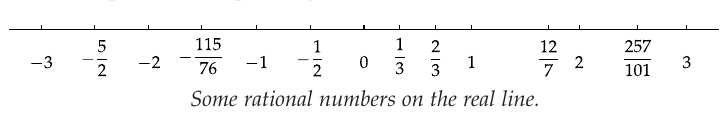
\includegraphics[scale=0.35]{real-line.png}
\end{figure}
\begin{itemize}
    \item if \( n\) is a positive integer then \( \frac{1}{n}\) is to the right of 0 by the length obtained by dividing the segment from \( 1 to 0\) in to \( n \) segments of equal length
\end{itemize}

\section{Is every Real Number a Rational}
\begin{figure}[h]
    \centering
    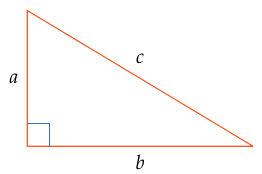
\includegraphics[scale=0.35]{irrational-geometry.png}
\end{figure}
\begin{itemize}
    \item \( c^{2} = a^{2} + b^{2} \). If \( a = 1, b = 1\) then \(c^{2} = 2 \). Then what rational number is \( c \)
    \item By trial and error, \( c = \left( \frac{99}{70} \right)^{2}  = \frac{9801}{4900}\) where the numerator just misses twice the denominator by 1. But this is not 2 but close to 2. Another number is \( \left( \frac{9369319}{6625109} \right)^{2} = 1.999999999999977\) , but not 2
    \item Greeks proved that it is impossible to find any rational number whose square is 2
\end{itemize}

\section{Proof: No rational number has a square equal to 2}
Let m and n are two integers
\[
    \left( \frac{m}{n} \right)^{2} = 2  
\]
By canceling any common factors, m and n are reduces to its lowest terms 

\[
    m^{2} = 2n^{2}
\]

this makes \(m^{2}\) even, hence \(m\) is an even. (The square of even is even and odd is odd). So \(m = 2k\) for some integer \(k\)

Substituting \(m = 2k\) in the equation gives, \(4k^{2} = 2n^{2} \), which results in 
\[
    2k^{2} = n^{2}
\]
which means \( n^{2}\) is even and therefore \(n \) is even
\\
\(\frac{m}{n} \) has common factors which contradicts the earlier assumption

\section{Irrational Number}

\begin{tcolorbox}[colback=yellow!5,
colframe=orange!80!black,
title=Irrational Number]
A real number that is not rational is \textbf{irrational number}
\end{tcolorbox}
\begin{itemize}
    \item \( \sqrt{2}\)
    \item \(3+\sqrt{2}\)
    \item \(8\sqrt{2}\)
\end{itemize}
\chapter{Algebra of Real Numbers}
\author{Nithin}

\section{Properties of Real Numbers}
\begin{itemize}
    \item \textbf{Commutative Properties}
    \begin{itemize}
        \item Addition: $a + b = b + a$
        \item Multiplication: $a \cdot b = b \cdot a$
    \end{itemize}
    \vspace{5pt}

    \item \textbf{Associative Properties}
    \begin{itemize}
        \item Addition: $(a + b) + c = a + (b + c)$
        \item Multiplication: $(a \cdot b) \cdot c = a \cdot (b \cdot c)$
    \end{itemize}
    \vspace{5pt}
    \item \textbf{Distributive Property}
    \begin{itemize}
        \item $a \cdot (b + c) = (a \cdot b) + (a \cdot c)$
    \end{itemize}
    \vspace{5pt}
    \item \textbf{Identity Elements}
    \begin{itemize}
        \item Additive Identity: $a + 0 = a$
        \item Multiplicative Identity: $a \cdot 1 = a$
    \end{itemize}
    \vspace{5pt}
    \item \textbf{Inverse Elements}
    \begin{itemize}
        \item Additive Inverse: $a + (-a) = 0$
        \item Multiplicative Inverse (if $a \neq 0$): $a \cdot \frac{1}{a} = 1$
    \end{itemize}
\end{itemize}

\begin{itemize}
    \vspace{5pt}
    \item \textbf{Closure Property}
    \begin{itemize}
        \item Real numbers are closed under addition, subtraction, multiplication, and division (except division by zero).
    \end{itemize}
\end{itemize}

\section{Inequalities,Intervals and Absolute Value}
\subsection{Inequalities}
\subsubsection{Transitivity}
\begin{itemize}
    \item If $a < b$ and $b < c$, then $a < c$
    \end{itemize}
\subsubsection{Multiplication}
Suppose $a < b$
\begin{itemize}
    \item If $c > 0$, then $ac < bc$
    \item If $c <  0$, then $ ac > bc$
\end{itemize}

\subsection{Exercise}
Find all number \( x \) such that 
\[\frac{x-8}{x-4} < 3 \]
Our first step  is to multiply by \(x-4\)
Here there are two conditions:
\begin{enumerate}
    \item \( x-4 > 0 \)
    \[ x -8 < 3(x-4)  \implies x-8 < 3x-12 \implies 2x > 4  \implies x > 2\]
    But our initial assumption is \(x-4 > 0 \implies x > 4 \). As \( 4 > 2 \), original inequality holds if \( x > 4\)
    \item \( x-4 < 0 \)
    \[ x-8 > 3(x-4) \implies  x < 2 \]
    Initial assumption is \( x<4 \). As \( 2 < 4\), inequality holds for \( x < 2 \)
\end{enumerate}
The original inequality holds true for \( [x < 2 ,  x > 4 ] \)
or 
\[  (-\infty, 2) \cup (4,\infty) \]

\subsection{Inequalities}
\subsubsection{Additive Inverse}
If \( a < b \) then \( -a > -b \)
Direction of inequalities has to be reversed when taking additive inverses on both sides 
\subsubsection{Multiplicative Inverse}
If \( a < b \)
\begin{itemize}
    \item If \(a > 0, b > 0\), then \(\frac{1}{a} > \frac{1}{b} \)
    \item If \(a < 0 < b\), then \(\frac{1}{a} < \frac{1}{b} \)
\end{itemize} 

\subsection{What is a Set?}
A \textbf{set} is a well-defined collection of distinct objects, called \textbf{elements} or \textbf{members} of the set.
\textbf{Representation of a Set:}
\begin{itemize}
    \item \textbf{Roster Form:} List elements inside curly braces:
    \[
    A = \{1, 2, 3, 4\}
    \]
    \item \textbf{Set-Builder Notation:} Describe properties of elements:
    \[
    A = \{x \mid x \text{ is a positive integer less than 5}\}
    \]
\end{itemize}
\subsubsection{Membership}
\begin{itemize}
    \item If \(x\) belongs to \(A\), write \(x \in A\).
    \item If \(x\) does not belong to \(A\), write \(x \notin A\).
\end{itemize}

\subsection{Types of Sets}
\begin{itemize}
    \item \textbf{Finite Set:} A set with a countable number of elements. \\
    Example: \(A = \{1, 2, 3, 4\} \)
    
    \item \textbf{Infinite Set:} A set with an uncountable or infinite number of elements. \\
    Example: \(\mathbb{N} = \{1, 2, 3, \dots\} \)

    \item \textbf{Empty/Null Set:} A set with no elements, denoted as \(\emptyset\) or \(\{\}\).

    \item \textbf{Subset:} \(A \subseteq B\) if every element of \(A\) is in \(B\).

    \item \textbf{Universal Set:} A set containing all objects under consideration, usually denoted by \(U\).

    \item \textbf{Power Set:} The set of all subsets of \(A\), denoted as \(P(A)\). \\
    Example: If \(A = \{1, 2\}\), then \(P(A) = \{\emptyset, \{1\}, \{2\}, \{1, 2\}\} \)
\end{itemize}

\subsection{Set Operations}
\subsubsection{Union (\(\cup\))}
Combines elements of two sets:
\[
    A \cup B = \{x \mid x \in A \text{ or } x \in B\}
\]
\subsubsection{Intersection (\(\cap\))}
Elements common to both sets:
\[
    A \cap B = \{x \mid x \in A \text{ and } x \in B\}
\]
\subsubsection{Difference (\(A - B\))}
Elements in \(A\) but not in \(B\):
\[
    A - B = \{x \mid x \in A \text{ and } x \notin B\}
\]
\subsubsection{Complement (\(A^c\))}
Elements not in the set \(A\):
\[
    A^c = \{x \mid x \notin A\}
\]
\subsubsection{Examples}
\begin{itemize}
    \item The set of natural numbers: \(\mathbb{N} = \{1, 2, 3, \dots\} \)
    \item The set of integers: \(\mathbb{Z} = \{\dots, -3, -2, -1, 0, 1, 2, 3, \dots\} \)
    \item The set of even numbers: \(\{2, 4, 6, \dots\} \)
\end{itemize}

\subsection{What is an Interval?}
An \textbf{interval} is a set of real numbers that includes all the numbers between two given endpoints.
Intervals describe ranges of values on the real number line and are widely used in mathematics.

\subsection{Types of Intervals}
\begin{itemize}
    \item \textbf{Closed Interval (\([a, b]\))}: Includes both endpoints \(a\) and \(b\).
    \[
    [a, b] = \{x \in \mathbb{R} \mid a \leq x \leq b\}
    \]
    Example: \([2, 5] = \{x \mid 2 \leq x \leq 5\} \).
    \vspace{5pt}

    \item \textbf{Open Interval (\((a, b)\))}: Excludes both endpoints \(a\) and \(b\).
    \[
    (a, b) = \{x \in \mathbb{R} \mid a < x < b\}
    \]
    Example: \((2, 5) = \{x \mid 2 < x < 5\} \).
\end{itemize}

\subsection{Half-Open or Half-Closed Intervals}
\begin{itemize}
    \item \textbf{Left-Closed, Right-Open (\([a, b)\))}:
    \[
    [a, b) = \{x \in \mathbb{R} \mid a \leq x < b\}
    \]
    Example: \([2, 5) = \{x \mid 2 \leq x < 5\} \).
    \vspace{5pt}

    \item \textbf{Left-Open, Right-Closed (\((a, b]\))}:
    \[
    (a, b] = \{x \in \mathbb{R} \mid a < x \leq b\}
    \]
    Example: \((2, 5] = \{x \mid 2 < x \leq 5\} \).
\end{itemize}

\subsection{Infinite Intervals}
\begin{itemize}
    \item \((a, \infty)\): All numbers greater than \(a\).
    \[
    (a, \infty) = \{x \in \mathbb{R} \mid x > a\}
    \]
    Example: \((3, \infty)\) includes all numbers greater than 3.

    \item \((-\infty, b)\): All numbers less than \(b\).
    \[
    (-\infty, b) = \{x \in \mathbb{R} \mid x < b\}
    \]
    Example: \((-\infty, 4)\) includes all numbers less than 4.

    \item \((-\infty, \infty)\): The entire real number line.
    \[
    (-\infty, \infty) = \mathbb{R}
    \]
\end{itemize}

\subsection{Summary of Interval Types}
\begin{tabular}{|c|c|c|}
    \hline
    \textbf{Type} & \textbf{Interval Notation} & \textbf{Description} \\
    \hline
    Closed         & \([a, b]\)      & Includes both endpoints \(a, b\) \\
    Open           & \((a, b)\)      & Excludes both endpoints \(a, b\) \\
    Half-Open Left & \([a, b)\)      & Includes \(a\), excludes \(b\) \\
    Half-Open Right & \((a, b]\)     & Excludes \(a\), includes \(b\) \\
    Infinite Left  & \((-\infty, b)\)& All \(x < b\) \\
    Infinite Right & \((a, \infty)\) & All \(x > a\) \\
    Entire Line    & \((-\infty, \infty)\) & All real numbers \\
    \hline
\end{tabular}

\subsection{What is Absolute Value?}
The \textbf{absolute value} of a number is its distance from zero on the number line, regardless of direction. It is always non-negative.
For a real number \(x\), the absolute value, denoted as \(|x|\), is defined as:
\[
|x| =
\begin{cases} 
x, & \text{if } x \geq 0, \\
-x, & \text{if } x < 0.
\end{cases}
\]
Breaking the absolute value: 
\begin{itemize}
    \item \( |f(x)| \leq c \quad \implies \quad -c \leq f(x) \leq c \)
    \item \( |f(x)| \geq c \quad \implies \quad f(x) \leq -c \quad \text{or} \quad f(x) \geq c \)
\end{itemize}

\subsection{Examples of Absolute Value}
\begin{itemize}
    \item \(|3| = 3\) \quad (because \(3 \geq 0\))
    \item \(|-5| = -(-5) = 5\) \quad (because \(-5 < 0\))
    \item \(|0| = 0\) \quad ( because \(0\) is neither positive nor negative)
\end{itemize}

\subsection{Properties of Absolute Value}
\begin{itemize}
    \item \textbf{Non-Negativity:} \(|x| \geq 0\) for all \(x\).
    \item \textbf{Identity Property:} \(|x| = 0 \quad \text{if and only if } x = 0\)
    \item \textbf{Multiplicative Property:} \(|x \cdot y| = |x| \cdot |y|\).
    \item \textbf{Triangle Inequality:} \( |x + y| \leq |x| + |y| \).
    \item \textbf{Distance Interpretation:} \(|x - y|\) represents the distance between \(x\) and \(y\).
\end{itemize}

\subsection{Exercises}
\subsubsection{Ball Bearings}
Ball bearings need to have extremely accurate sizes to work correctly. The ideal diameter of a particular ball bearing is 0.8 cm, but a ball bearing is declared acceptable if the error in the diameter size is less than 0.001 cm. Write the inequality for acceptance criteria
\subsubsection{Solution}
The ball bearings are acceptable if the diameter \(d\) satisfies:
\[
|d - 0.8| < 0.001
\]

\subsection{Exercises}
Find all numbers \(t \) such that \( |3t-4| = 10\)
Solution :
\[ 3t -4  = 10  \; or \; 3t-4 = -10  \implies t = \frac{14}{3}, t = -2 \]

\subsection{Exercise}
Find all numbers \(x\) such that \( \left| \frac{3x-5}{x-1} \right|< 2 \)
Solution :
\[ |3x-5| < 2 |x-1| \]
\begin{enumerate}
    \item \(x-1 > 0 \)
\end{enumerate}
Breaking the absolute value:
\begin{flalign}
    &\implies -2(x-1) < 3x-5 < 2(x-1) = -2x + 7 < 3x < 2x + 3  \ 
    &\implies 3x > -2x+7   \; \& \; 3x < 2x + 3  
\end{flalign}

\subsection{Exercise}
Solving for \( 3x < 2x + 3\)
\begin{flalign}
    &\implies x < 3 \\
\end{flalign}
Solving for \(3x > -2x+7 \)
\begin{flalign}
    &\implies 3x > -2x+7 \implies 5x > 7 \implies x > 7/5 \\
    &\implies x \in (7/5,3) 
\end{flalign}

\subsection{Exercise} 
\begin{enumerate}
    \setcounter{enumi}{1}
    \item \(x-1 < 0 \implies x < 1 \)
\end{enumerate}
\begin{flalign}
    &\implies |3x-5| < 2 |x-1| == |3x-5| < -2(x-1) \\
    &\implies         3x-5 < -2(x-1) \; \text{ and } \; -(3x-5) < -2(x-1) \\
    &\implies  3x-5 < -2(x-1)  \; \text{ and } \; 3x-5 > 2(x-1) 
\end{flalign}
\begin{flalign}
    &3x-5 < -2(x-1) \implies  3x < -2x+7 \implies 5x < 7 \implies x < 7/5 \\
    &\implies 3x-5 > 2(x-1) \implies 3x > 2x + 3 \implies x > 3 
\end{flalign}
Here \( x > 3\) is inconsistent with our assumption \(x < 1\). So for \(x<1\) there are no values of \(x\) satisfying the inequality
\chapter{Introduction to Functions}
\author{Nithin}

\section{Domain,Range and Equality}

\subsection{What is a Function ?}
A function associates every number in some set of real numbers, called the domain of the function, with exactly one real number.

\subsection{Domain}
If a function is defined by a formula, with no domain specified, then the domain is assumed to be the set of all real numbers for which the formula makes sense and produces a real number.

\subsubsection{Example 3}
Find the domain of the function \(f\)  defined by \[f (x) = (3x-1)^2 \]

\subsubsection{Example 4}
Find the domain of the function \(f\) defined by \[h (t) = \frac{t^2 + 3t + 7}{t-4} \]

\subsubsection{Example 6}
Find the domain of the function g defined by \[g(x) = \sqrt{|x|-5}\]

\subsection{Range}
The range of a function \(f\) is the set of all numbers \(y\) such that \(f (x) = y\) for at least one \(x\) in the domain of \(f\).

\subsubsection{Example 4}
The domain of \(f\) is the interval \( [2, 5] \), with \(f\) defined on this interval by the equation \(f (x) = 3x + 1\).
Solution:
\[ y = f(x) = 3x+1 \]
\[ 2 \leq \frac{y-1}{3} \leq 5. \]
\[ 7 \leq y \leq 16. \]

\subsubsection{Example 5}
The domain of \(g\) is the interval \([1,20]\), with \(g\) defined on this interval by the equation
\[ g(x) = |x - 5|. \]
Is \(2\) in the range of \(g\)?
Solution:
\[ y =  |x-5| \]
for \(x-5>0 \),\(y = x-5 \implies x = y+5 \)
\[ 5 < y+5 \leq 20  \implies  0 < y \leq 15 \]
for \(x-5<0 \), \(y = -(x-5) \implies y = -x+5 \implies 5-y = x \)
\[ 1 \leq 5-y \leq 5  \implies -4 \leq -y \leq 0 \implies  4 \geq y \geq 0 \]

\subsection{Equality of Functions}
Two functions are equal if and only if they have the same domain and the same value at every number in that domain.

\subsubsection{Example}
Suppose \(f\) is the function whose domain is the set of real numbers, with \(f\) defined on this domain by
\[f (x) = x^2\]
Suppose \(g\) is the function whose domain is the set of positive numbers, with \(g\) defined on this domain by
\[g(x) = x^2\]
Are \(f\) and \(g\) equal functions?

\subsubsection{Example 2}
Suppose \(f\) and \(g\) are functions whose domain is the set consisting of the two numbers \(\{1, 2\}\) with \(f\) and \(g\) defined on this domain by the formulas
\[f (x) = x^2\] and \(g(x) = 3x-2\).
Are \(f\) and \(g\) equal functions?

\section{Analytical Geometry}
\subsection{What is Analytic Geometry?}
\begin{itemize}
    \item \textbf{Analytic Geometry} (also called \textit{coordinate geometry} or \textit{Cartesian geometry}) bridges algebra and geometry.
    \item It uses a coordinate system to study geometric shapes and properties.
    \item Geometric objects are represented as algebraic equations.
\end{itemize}

\subsection{Co-ordinate Plane}
\begin{figure}[h]
    \centering
    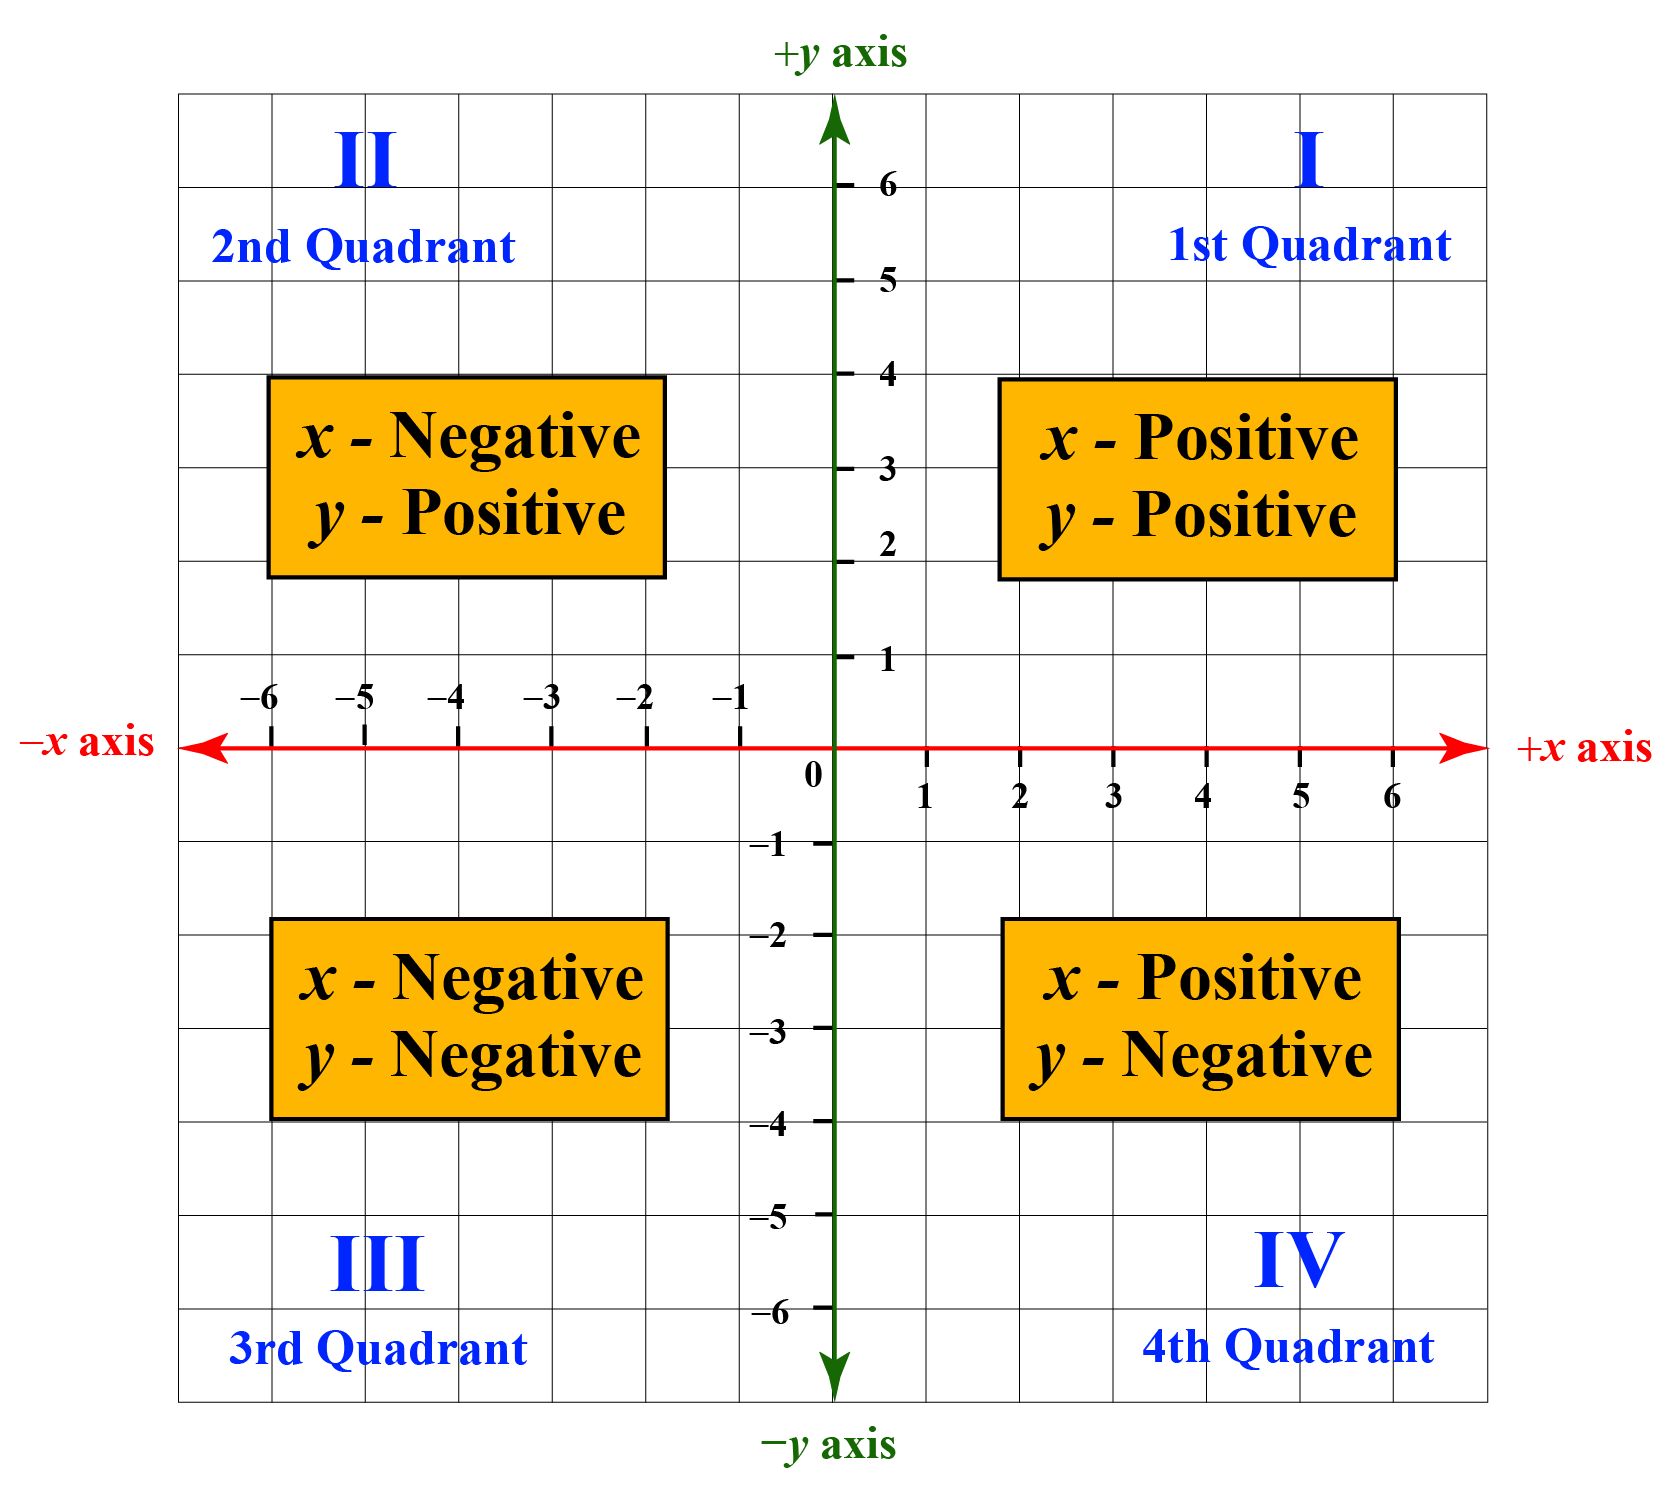
\includegraphics[scale=0.23]{cartesian.png}
\end{figure}
The plane with this system of labeling is often called the \textbf{Cartesian plane} in honor of the French mathematician Rene Descartes(1596-1650), who described this technique in his 1637 book Discourse on Method.

\subsection{Graph Functions}
The graph of a function \(f\) is the set of points of the form \(x, f (x)\) as x varies over the domain of \(f\).

\subsubsection{Graphs}
\begin{figure}[h]
  \centering
  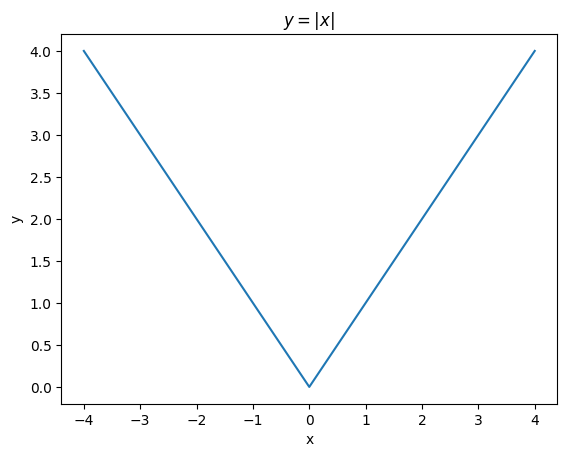
\includegraphics[scale=0.3]{graph.png}
\end{figure}
\begin{figure}[h]
  \centering
  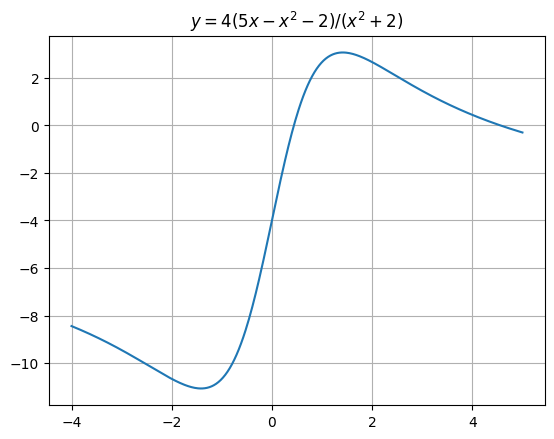
\includegraphics[scale=0.3]{graph2.png}
\end{figure}

\subsection{Checking for a function: Vertical line test}
The line \(x=1\) intersects the curve at two points. That is that for each \(x\) value there are multiple \(y\) values which is contradicting to definition of a function.
\subsubsection{Vertical Line Test}
A set of points in the coordinate plane is the graph of some function if and only if every vertical line intersects the set in at most one point.

\section{Average Rate of change}
The rate of change describes how an output quantity changes relative to the change in the input quantity. The unit on a rate of change.
The \textbf{average rate of change} of a function \(f\) over an interval \([x_{1}, x_{2}]\) is given by
\[ =\frac{\Delta y}{\Delta x} =\frac{f(x_{2}) - f(x_{1})}{x_{2} - x_{1}} \]

\subsection{Increasing, Decreasing and Constant Functions}
\begin{figure}
  \centering
  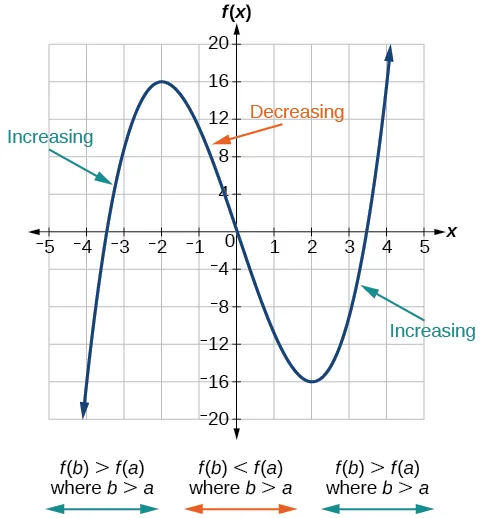
\includegraphics[scale=0.3]{inc-dec.png}
\end{figure}

\subsubsection{Increasing Function}
A function \(f\) is said to be increasing on an interval \((a, b)\) if for any \(x_{1}, x_{2}\) in \((a, b)\) with \(x_{1} < x_{2}\), we have \(f(x_{1}) < f(x_{2})\) or it has a positive rate of change over the interval.

\subsubsection{Decreasing Function}
A function \(f\) is said to be decreasing on an interval \((a, b)\) if for any \(x_{1}, x_{2}\) in \((a, b)\) with \(x_{1} < x_{2}\), we have \(f(x_{1}) > f(x_{2})\) or it has a negative rate of change over the interval.

\subsubsection{Constant Function}
A function \(f\) is said to be constant on an interval \((a, b)\) if for any \(x_{1}, x_{2}\) in \((a, b)\) with \(x_{1} < x_{2}\), we have \(f(x_{1}) = f(x_{2})\) or it has a zero rate of change over the interval.

\subsection{Local Maxima and Local Minima}
\begin{figure}
  \centering
  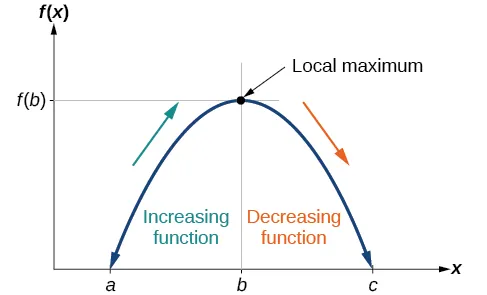
\includegraphics[scale=0.5]{max-min.png}
\end{figure}

\subsubsection{Local Maximum}
A function \(f\) has a \textbf{local maximum} at \(x = c\) if there exists an interval \((a, b)\) containing \(c\) such that
\[ f(c) \geq f(x) \quad \text{for all } x \in (a, b) \]

\subsubsection{Local Minimum}
A function \(f\) has a \textbf{local minimum} at \(x = c\) if there exists an interval \((a, b)\) containing \(c\) such that
\[ f(c) \leq f(x) \quad \text{for all } x \in (a, b) \]

\section{Function Transformation}
\subsection{Vertical Transformations}
\subsubsection{Shifting a graph up or down}
Suppose \(f \) is a function and \(a > 0\). Upshift \(g\) and  Downshift \(h\) by
\[g(x) = f (x) + a \;\; h(x) = f (x) - a \]
\begin{figure}[h]
  \centering
  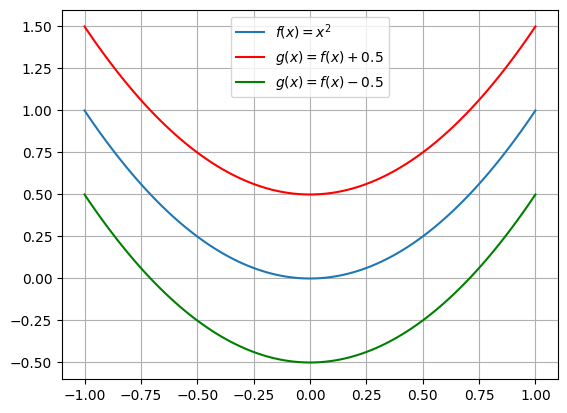
\includegraphics[scale=0.4]{vertical_shift.png}
\end{figure}

\subsubsection{Vertical Stretch}
Suppose \(f\) is a function and \(c > 0\). Define a function \(g\) by
\[g(x) = c f (x)\]
\begin{figure}[h]
  \centering
  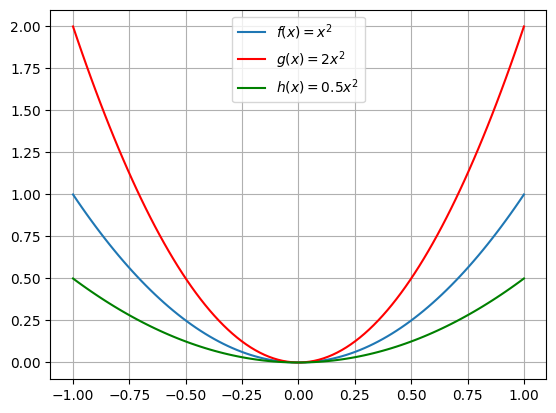
\includegraphics[scale=0.5]{vertical_stretch.png}
\end{figure}

\subsubsection{Flipping along the Vertical Axis}
Vertical fliiping of \(f(x) \) is
\[g(x) = - f (x) \]
\begin{figure}[h]
  \centering
  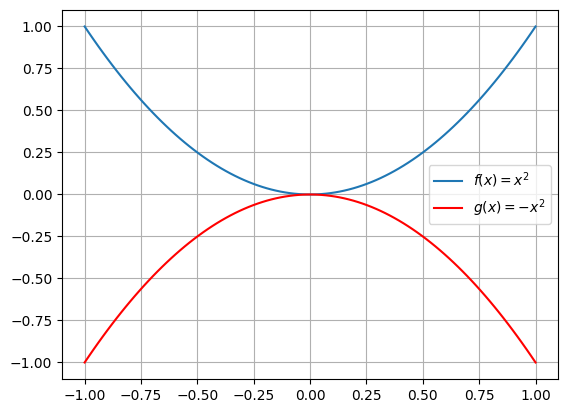
\includegraphics[scale=0.5]{vertical_flip.png}
\end{figure}

\subsection{Horizontal Transformation}
\subsubsection{Horizontal Shift}
\[g(x) = f(x+a), h(x) = f(x-a)\]
\begin{figure}[h]
  \centering
  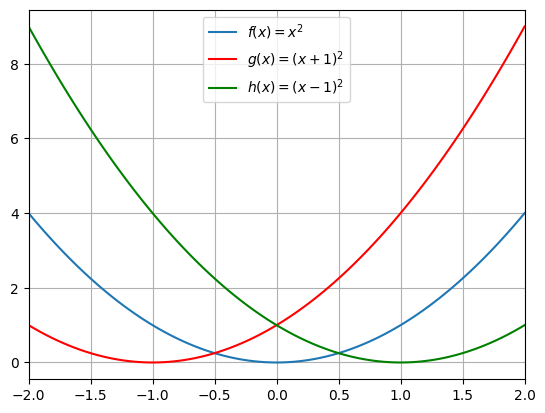
\includegraphics[scale=0.5]{horizontal-shift.png}
\end{figure}

\subsubsection{Horizontal Stretching}
\[g(x) = f(cx)\]
\begin{figure}[h]
  \centering
  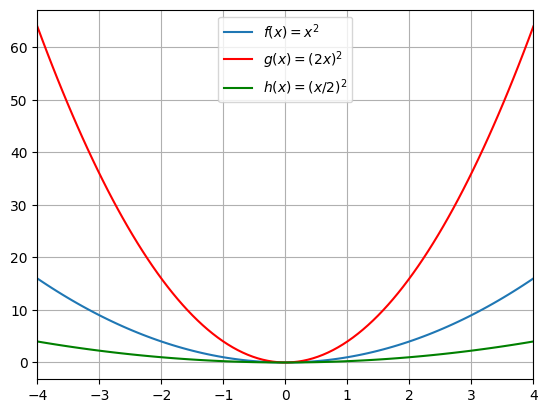
\includegraphics[scale=0.55]{horizontal-stretch.png}
\end{figure}

\subsection{Flipping ac the Vertical Axis}
\subsubsection{Horizontal Stretching}
\[g(x) = f(-x)\]
\begin{figure}[h]
  \centering
  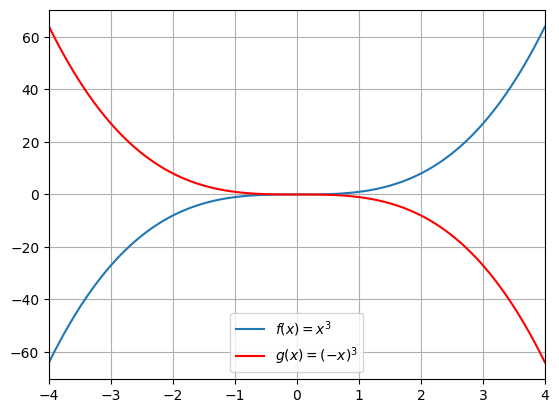
\includegraphics[scale=0.55]{vertical-axis-flip.png}
\end{figure}

\subsection{Combinations of vertical Transformation}
\begin{figure}[h]
  \centering
  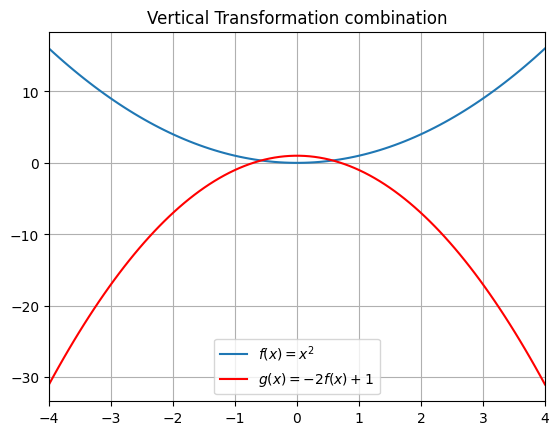
\includegraphics[scale=0.55]{vertical_combination.png}
\end{figure}

\subsection{Even Functions}
\[ f(-x) = f(x) \quad \text{for all } x \text{ in the domain} \]
Example: \( f(x) = x^2, \quad f(x) = \cos x \)
The graph of an even function is symmetric across the vertical axis.
\begin{figure}
\centering
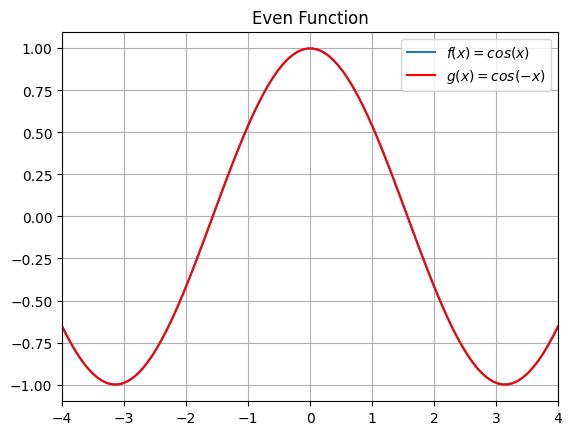
\includegraphics[width=0.45\linewidth]{even.png}
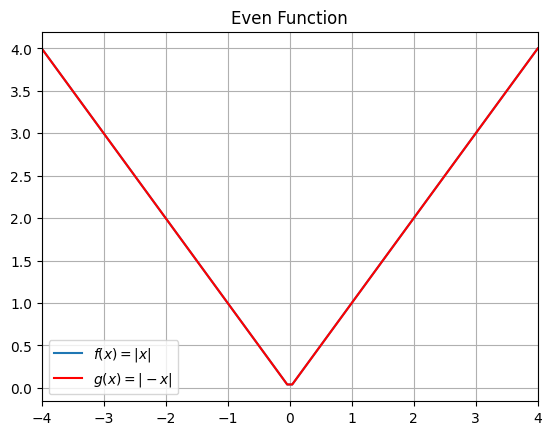
\includegraphics[width=0.45\linewidth]{even2.png}
\end{figure}

\subsection{Odd Function}
\[ f(-x) = -f(x) \quad \text{for all } x \text{ in the domain} \]
Example: \( f(x) = x^3, \quad f(x) = \sin x \)
The graph of an even function is symmetric if flipped or rotated 18 across the origin.
\begin{figure}
\centering
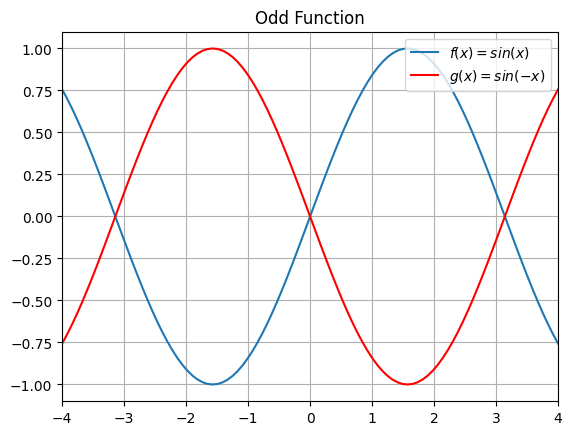
\includegraphics[width=0.45\linewidth]{odd.png}
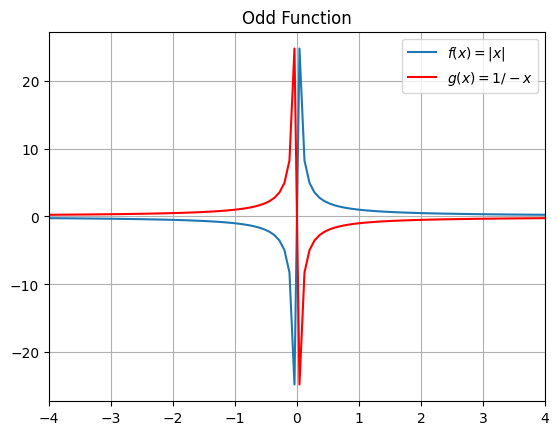
\includegraphics[width=0.45\linewidth]{odd2.png}
\end{figure}

\section{Function Composition}
\subsection{Algebra of Functions}
Suppose \(f\) and \(g\) are functions. We can define new functions from \(f\) and \(g\) as follows: \\
\textbf{Sum:}
\[ (f+g)(x) = f(x) + g(x) \]
\textbf{Difference:}
\[ (f-g)(x) = f(x) - g(x) \]
\textbf{Product:}
\[ (f\cdot g)(x) = f(x) \cdot g(x) \]
\textbf{Quotient:}
\[ \left(\frac{f}{g}\right)(x) = \frac{f(x)}{g(x)} \quad \text{provided } g(x) \neq 0. \]
\textbf{Note:} If \(f\) and \(g\) have domains \(D_f\) and \(D_g\), then these operations are defined on the intersection \(D_f \cap D_g\). In the case of the quotient, it is defined on
\[ \{x \in D_f \cap D_g : g(x) \neq 0\}. \]

\subsection{Exercise}
\( f(x)  = \sqrt{x-3}\) and \(g(x) = \sqrt{8 - x } \)
Evaluate
\begin{enumerate}
  \item[a.] \((f+g)(x)\)
  \item[b.]  \((fg)(x)\)
  \item[c.] Find the domain of above
\end{enumerate}
Sol:
\begin{enumerate}
  \item[a.] \(\sqrt{x-3} + \sqrt{8-x} \)
  \item[b.] \(\sqrt{(x-3)(8-x)} \)
  \item[c.]  Domian of \begin{enumerate}
    \item[a.] \(x\geq 3 \)
    \item[b.] \(x \leq 8 \)
    \item[c.] \( 3 \leq x \leq 8 \)
  \end{enumerate}
\end{enumerate}

\subsection{Function Composition}
\subsubsection{Definition:}
If \( f(x) \) and \( g(x) \) are functions, then the composition of \( f \) and \( g \), denoted by \( f \circ g \), is defined by
\[ (f \circ g)(x) = f(g(x)). \]
\textbf{Example:}
Consider the function
\[ h(x) = \sqrt{x+3}. \]
We can express \( h(x) \) as a composition of two functions \( f \) and \( g \) where:
\[ f(x) = \sqrt{x} \quad \text{and} \quad g(x) = x+3. \]
Then,
\[ h(x) = f(g(x)) = f(x+3) = \sqrt{x+3}. \]

\subsection{Exercise}
\( f(x) = \frac{1}{x-4} \) and \( g(x) = x^{2} \)
\begin{enumerate}
  \item \(f \circ g \)
  \item \( g \circ f \)
  \item domian of \(f \circ g \)
  \item domain of \( g \circ f \)
\end{enumerate}
Sol:
\begin{enumerate}
  \item  \(f(g(x)) = \frac{1}{x^{2} - 4}\)
  \item \(g(f(x)) = (\frac{1}{x-4})^{2}\)
  \item \(R - \{-2,2\} \)
  \item \(R - \{4\} \)
\end{enumerate}

\subsection{Composition Machine}
\begin{figure}
  \centering
  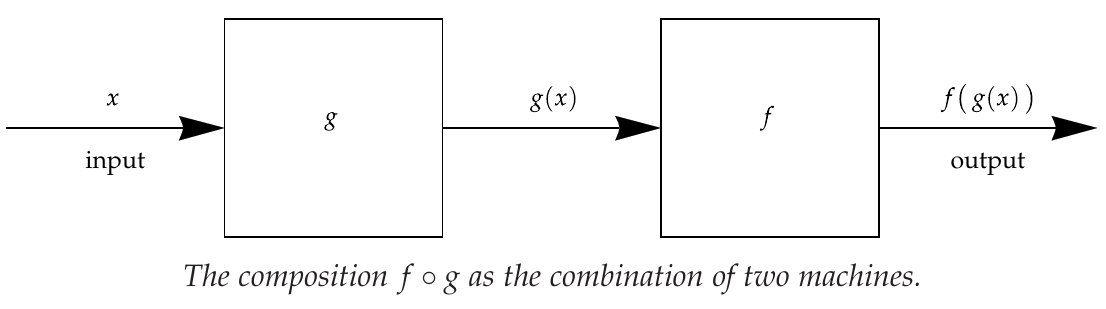
\includegraphics[scale=0.3]{composition.png}
\end{figure}

\subsection{Excersise}
\textbf{Problem:} Suppose your cell phone company charges \(\$0.05\) per minute plus \(\$0.47\) for each call to China.
\begin{enumerate}
  \item[(a)] Find a function \(p\) that gives the amount charged by your cell phone company for a call to China as a function of the number of minutes \(m\).
  \item[(b)] Suppose the tax on cell phone bills is 6\% plus \(\$0.01\) for each call. Find a function \(t\) that gives your total cost, including tax, for a call to China as a function of the amount charged by your cell phone company.
  \item[(c)] Explain why the composition \(t \circ p\) gives your total cost, including tax, of making a cell phone call to China as a function of the number of minutes.
  \item[(d)] Compute a formula for \(t \circ p\).
  \item[(e)] What is your total cost for a ten-minute call to China?
\end{enumerate}

\subsection{Solution}
\textbf{(a)} The company charges \(\$0.05\) per minute plus a fixed charge of \(\$0.47\) per call. Hence, the pre-tax charge function is
\[ p(m)=0.05m+0.47. \]
\textbf{(b)} The tax on the cell phone bill is 6\% of the pre-tax amount plus an additional \(\$0.01\) per call. Thus, if the pre-tax charge is \(x\), the total cost function (including tax) is
\[ t(x)=1.06x+0.01. \]
\textbf{(c)} The composition \(t \circ p\) means we first compute the pre-tax charge \(p(m)\) for a call of \(m\) minutes, and then we apply the tax function \(t\) to this amount. In other words, \(t(p(m))\) gives the total cost, including tax, as a function of the number of minutes.
\textbf{(d)} To compute the composition, substitute \(p(m)\) into \(t\):
\[ (t \circ p)(m)=t(p(m))=1.06\bigl(0.05m+0.47\bigr)+0.01. \]
Distribute \(1.06\):
\[ 1.06(0.05m)=0.053m \quad \text{and} \quad 1.06(0.47)=0.4982. \]
Thus,
\[ (t \circ p)(m)=0.053m+0.4982+0.01=0.053m+0.5082. \]
\textbf{(e)} For a ten-minute call (\(m=10\)):
\[ (t \circ p)(10)=0.053(10)+0.5082=0.53+0.5082=1.0382. \]
Rounded to the nearest cent, the total cost is approximately \(\$1.04\).

\subsection{Identity Function}
The identity function is defined by
\[ I(x) = x \quad \text{for every number } x. \]
The function \(I\) is the identity for composition. If \(f\) is any function, then
\[ f \circ I = I \circ f = f. \]

\subsection{Decomposing the Functions}
\subsubsection{Function Decomposition}
\[ T(y) = \frac{|y^{2} -3|}{|y^{2} - 7|} \]
Sol:
\[f(y) = |y|, g(y) = \frac{y^{2}-3}{y^{2}-7} \]
\[ f(y) = \frac{|y-3|}{|y-7|}, g(y) = y^{2}\]
Composition is associative if \(f,g, h\) are functions then
\[(f \circ g) \circ h  = f \circ (g \circ h) \]

\subsection{Example}
\subsubsection{Composition of three functions}
\[T(x) = \left| \frac{x^{2}-3}{x^{2} - 7}  \right| \]
Sol:
\[f(x) = |x|, g(x) = \frac{x-3}{x-7}, h(x) = x^{2}\]

\subsection{Linear Functions}
A linear function is a function \(h\) of the form
\[h(x) = mx + b\]
where \(m\) and \(b\) are numbers.

\subsection{Linear Functions as Composition}
\subsubsection{Vertical Transformations as Compositions}
A funtion \(g(x)\) is defined by
\[g(x)= -2f(x)+1\]
Write \(g(x)\) as a the composition of a linear function with \(f(x)\)
\[h(x) = -2x + 1 \]
\[\implies g(x) = h(f(x)) \implies g = h \circ f \]

\subsubsection{Horizontal Transformations as Compositions}
A funtion \(g(x)\) is defined by
\[g(x)= f(2x)+1\]
Write \(g(x)\) as a the composition of a linear function,  \(f(x)\) and other linear function
\[h(x) = x + 1, p(x) = 2x \]
\[\implies g(x) = h(f(p(x))) \implies g = h \circ f \circ p \]

\section{Inverse Functions}
\subsection{Inverse Function: Example}
Consider the function \( f: \mathbb{R} \to \mathbb{R} \) defined by
\[ y = \frac{9}{5}x + 32, \]
which converts a temperature \( x \) in Celsius to Fahrenheit \( y \). 
The inverse function \( f^{-1} \) converts Fahrenheit back to Celsius:
\[ f^{-1}(y) = \frac{5}{9}(y - 32). \]
Verifying that these functions are inverses:
\[ f^{-1}(f(x)) = \frac{5}{9}\Bigl(\frac{9}{5}x + 32 - 32\Bigr) = x, \]
\[ f(f^{-1}(f)) = \frac{9}{5}\Bigl(\frac{5}{9}(y - 32)\Bigr) + 32 = y. \]

\subsection{One-to-One Function}
A function \(f\) is called one-to-one if for each number \(y\) in the range of \(f\) there is
exactly one number \(x\) in the domain of \(f\) such that \(f (x) = y\).

\subsection{Inverse Function}
\subsubsection{Definition}
Suppose \( f \) is a one-to-one function.
\begin{itemize}
  \item If \( y \) is in the range of \( f \), then \( f^{-1}(y) \) is defined to be the number \( x \) such that \( f(x) = y \).
  \item The function \( f^{-1} \) is called the \emph{inverse function} of \( f \).
\end{itemize}
\textbf{Short version:}
\begin{itemize}
  \item \( f^{-1}(y) = x \) means \( f(x) = y \).
\end{itemize}

\begin{figure}
  \centering
  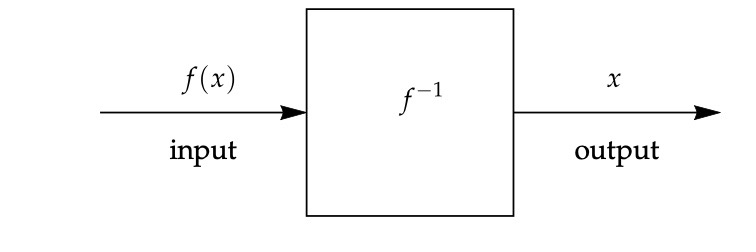
\includegraphics[scale=0.4]{inverse.jpeg}
\end{figure}

\subsection{Domain and Range of an Inverse Function}
If \( f \) is a one-to-one function, then:
\begin{itemize}
  \item The domain of \( f^{-1} \) equals the range of \( f \).
  \item The range of \( f^{-1} \) equals the domain of \( f \).
\end{itemize}

\subsection{Increasing and Decreasing Function}
\subsubsection{Increasing}
A function \(f\) is called increasing if \(f (a) < f (b)\) whenever \(a < b\) and \(a, b \) are in
the domain of \(f\).

\subsubsection{Decreasing}
A function \(f\) is called decreasing if \(f (a) >  f (b)\) whenever \(a < b\) and \(a, b \) are in
the domain of \(f\).

\subsubsection{Increasing and decreasing functions are one-to-one}
\begin{itemize}
  \item Every increasing function is one-to-one
  \item Every decreasing function is one-to-one.
\end{itemize}

\subsection{Exercise}
\begin{figure}
  \centering
  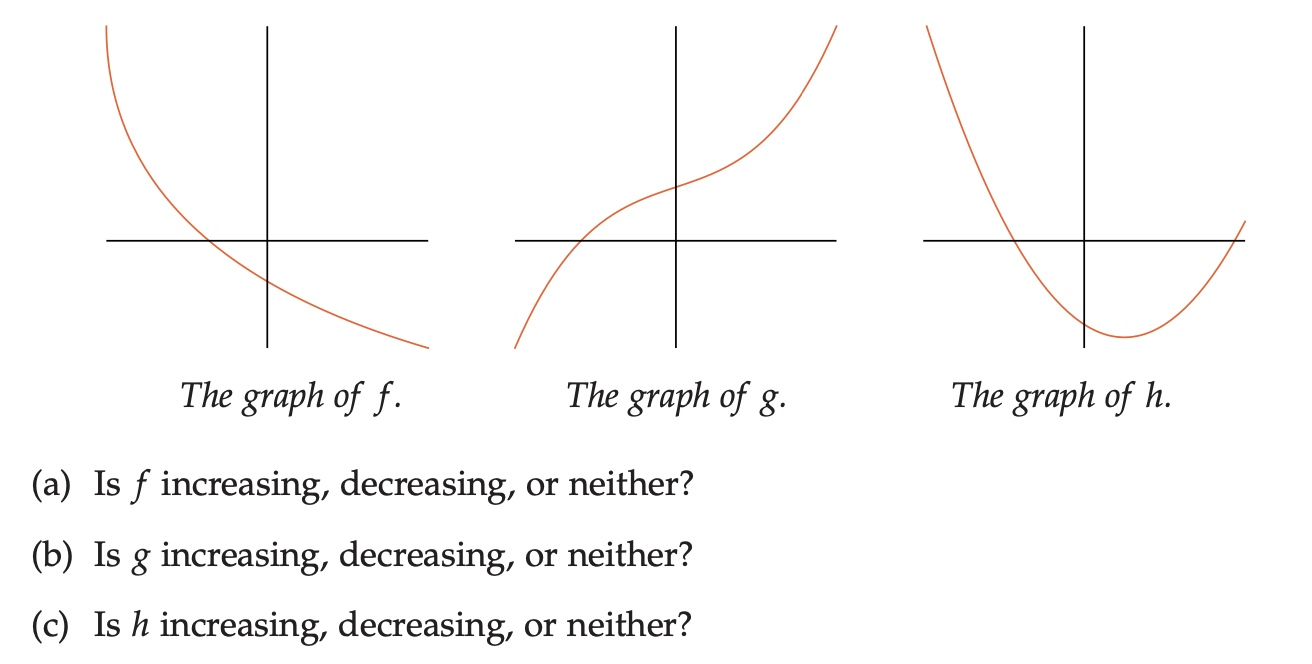
\includegraphics[scale=0.2]{increase.jpeg}
\end{figure}
\begin{enumerate}
  \item[a.] Decreasing
  \item[b.] Increasing
  \item[c.] Neither
\end{enumerate}

\subsection{Do all one-to-one maps are increasing or decreasing ?}
% \begin{figure}
%   \centering
%   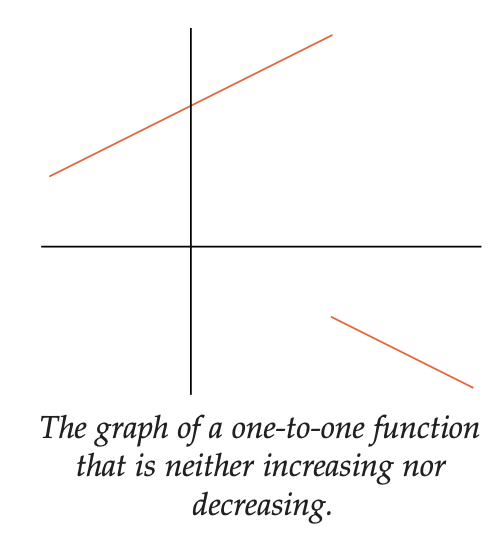
\includegraphics[scale=0.6]{pics/non-increse-decrese.png}
% \end{figure}

\subsection{Increasing and Decreasing Functions}
\subsubsection{Inverses of increasing and decreasing functions}
\begin{itemize}
  \item The inverse of an increasing function is increasing.
  \item The inverse of a decreasing function is decreasing.
\end{itemize}

\chapter{Linear,Quadratic, Polynomial and Rational Functions}
\author{Nithin}

\section{Lines and Linear Function}
\subsection{Slope}
\begin{figure}
  \centering
  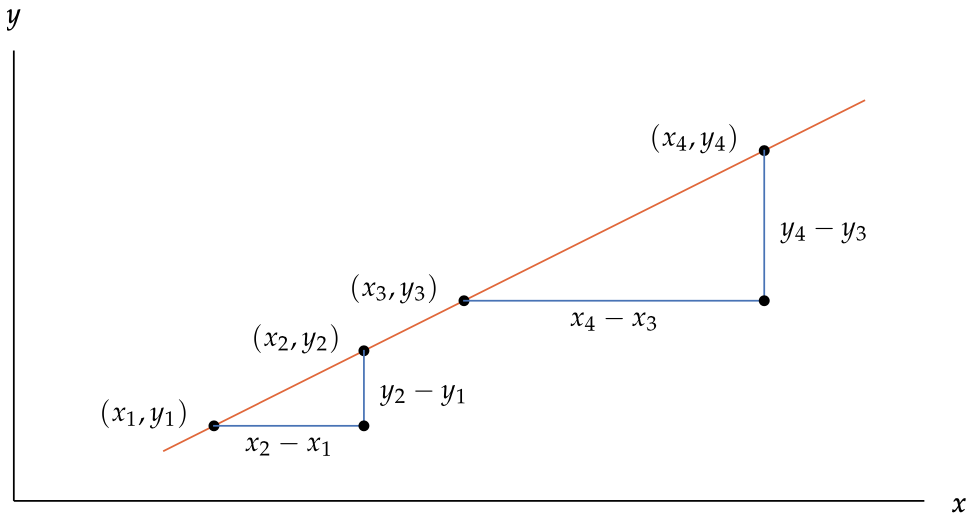
\includegraphics[scale=0.25]{slope.png}
\end{figure}
\[\frac{y_{2} - y_{1}}{x_{2} - x_{1}} = \frac{y_{4} - y_{3}}{x_{4} - x_{3}}\]

If \(x_{1},y_{1}\) and \(x_{2},y_{2}\) are any two points on a line with \(x_{1} \neq x_{2}\), then the \textbf{slope} of the line is
\[\frac{y_{2} - y_{1}}{x_{2} - x_{1}}\]

\begin{figure}
  \centering
  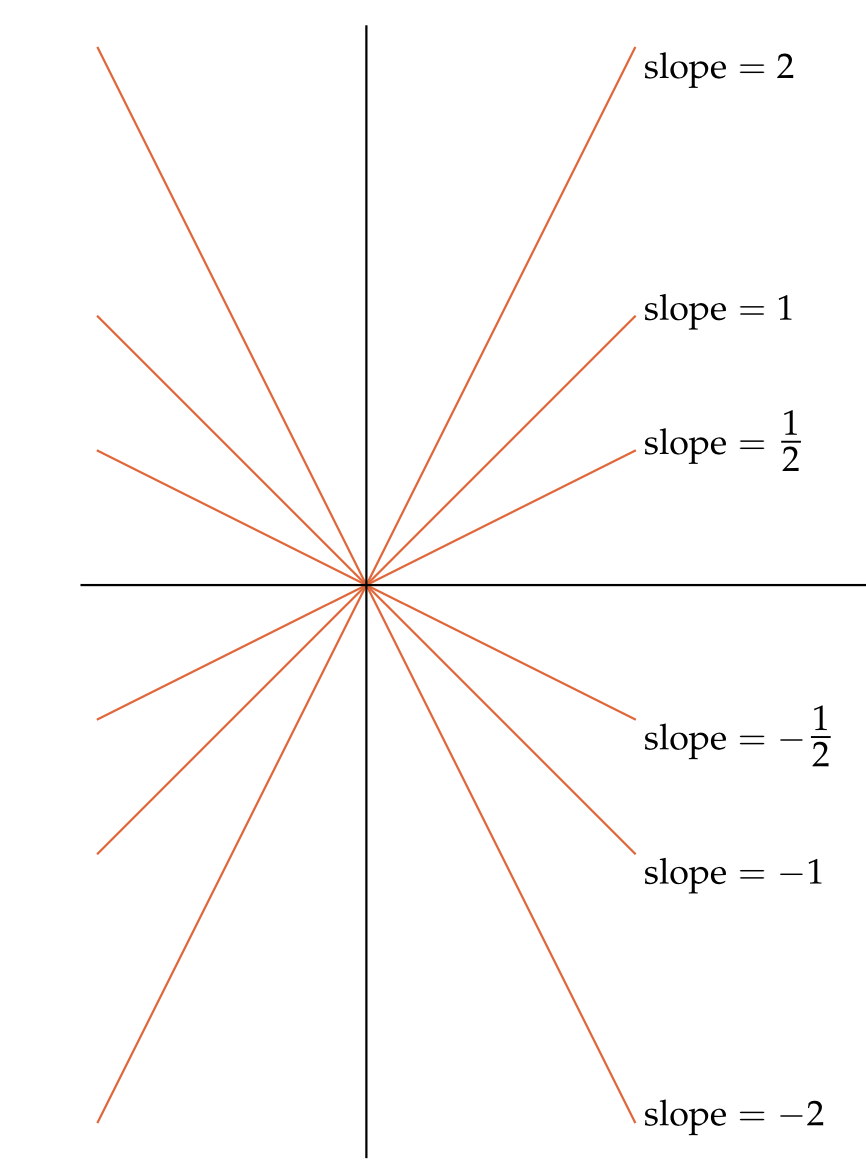
\includegraphics[width=0.5\linewidth]{slope2.png}
\end{figure}
\textbf{Key Points:}
\begin{itemize}
    \item Positive slope slands up from left to right
    \item Negative slope slands down from left to right
    \item Horizontal line has slope = 0
    \item Vertical line has no slope
\end{itemize}

\subsection{Line Equation}
\subsubsection{Slope and one point on it}
The line in the xy-plane that has slope \(m\) and contains the point \((x1, y1)\) is given by the equation
\[y - y_{1} = m(x  -  x_{1})\]
\begin{figure}
  \centering
  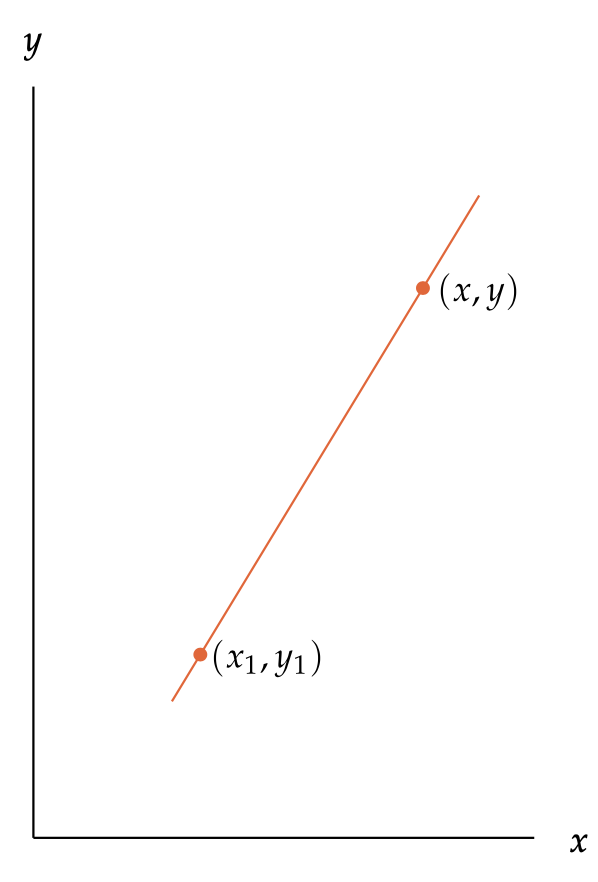
\includegraphics[width=0.5\linewidth]{line1.png}
\end{figure}

\subsubsection{Slope and \(y\) intercept}
The line in the xy-plane with slope \(m\) that intersects the \(y\) axis at \(0,b\) is given by the equation
\[y = mx+b\]
\begin{figure}
  \centering
  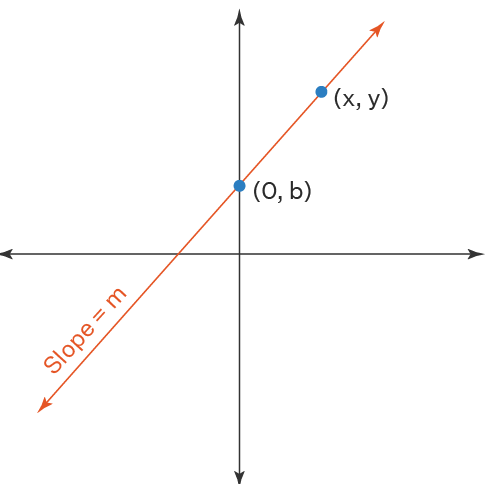
\includegraphics[width=0.5\linewidth]{line2.png}
\end{figure}

The line in the xy-plane that contains the points \(x_{1},y_{1}\) and \(x_{2}, y_{2}\) where \(x_{1} \neq x_{2}\), is
\[y-y_{1} = \left( \frac{y_{2} - y_{1}}{x_{2} - x_{1}} \right) (x-x_{1})\]

\subsection{Linear Function}
A \textbf{linear function} is a function \(f\) of the form
\[f(x) = mx + b\]
where \(m\) and \(b\) are numbers.

\subsubsection{Linear Functions: Origin vs Y-Intercept}
\textbf{Example 1: Temperature Conversion}
\begin{itemize}
    \item Correct formula: \( F = 1.8C + 32 \) (Starts at 32°F)
    \item Incorrect direct proportion: \( F' = 1.8C \) (Wrong assumption)
\end{itemize}
\textbf{Example 2: Weight Conversion}
\begin{itemize}
    \item True conversion: \( lb = 2.205 \times kg \) (Passes through origin)
    \item Shipping charge model: \( lb' = 5 + 2.205 \times kg \) (Has minimum billable weight or fixed cost markup)
\end{itemize}
\begin{figure}
\centering
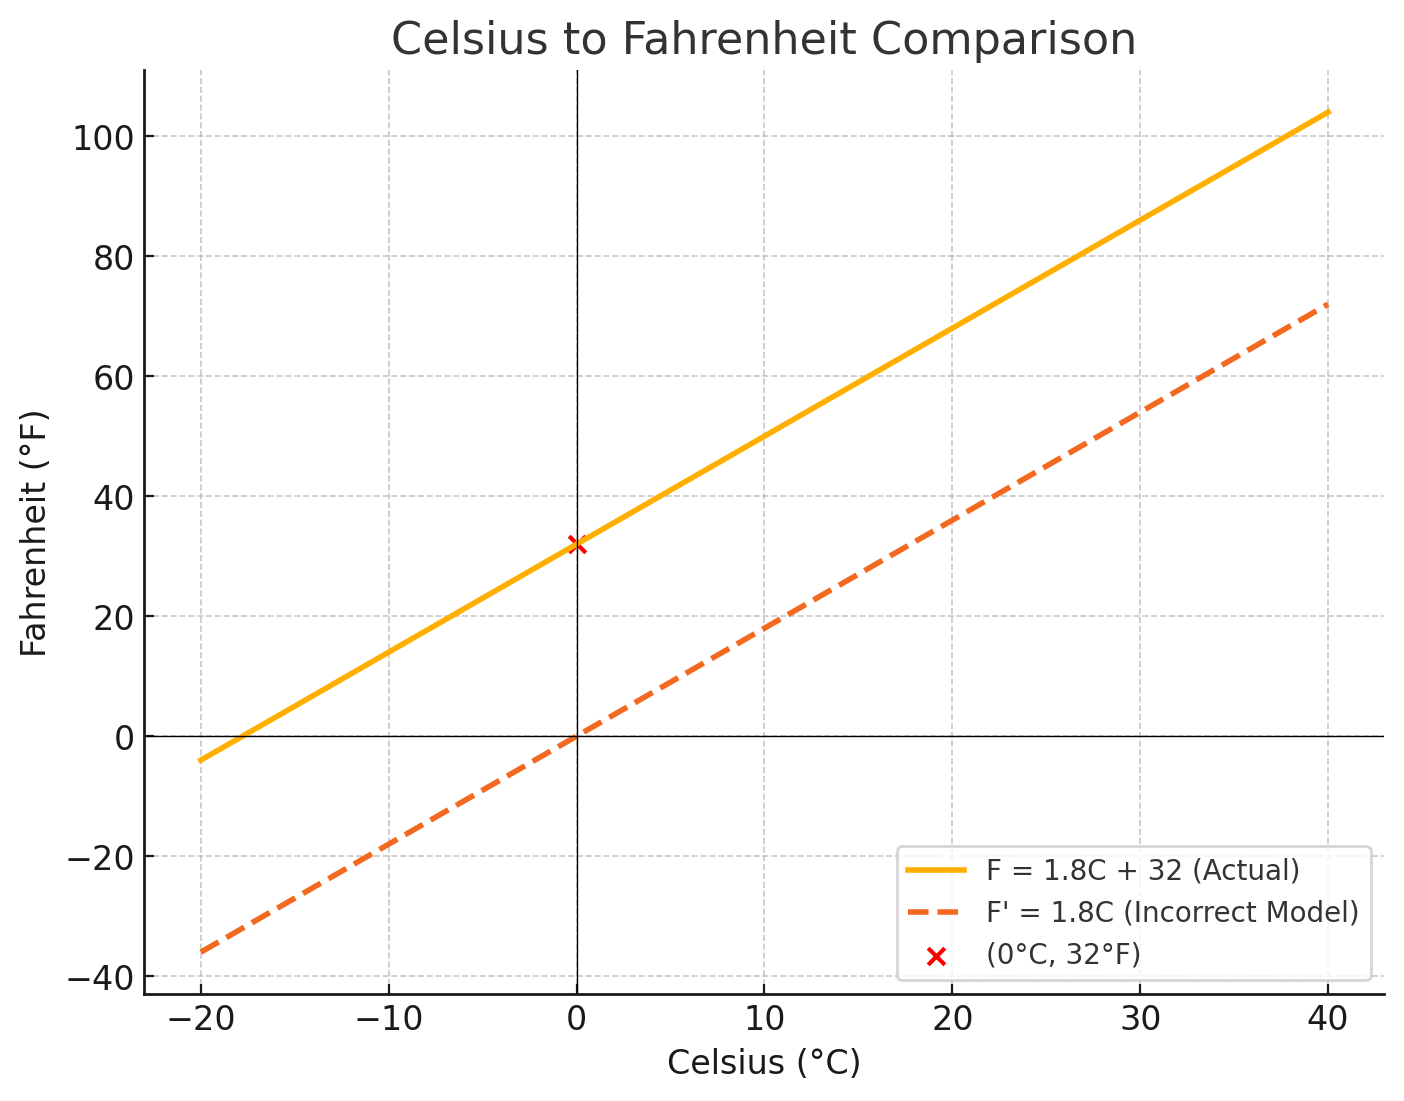
\includegraphics[width=0.45\linewidth]{Celsius to Fahrenheit Comparison.png}
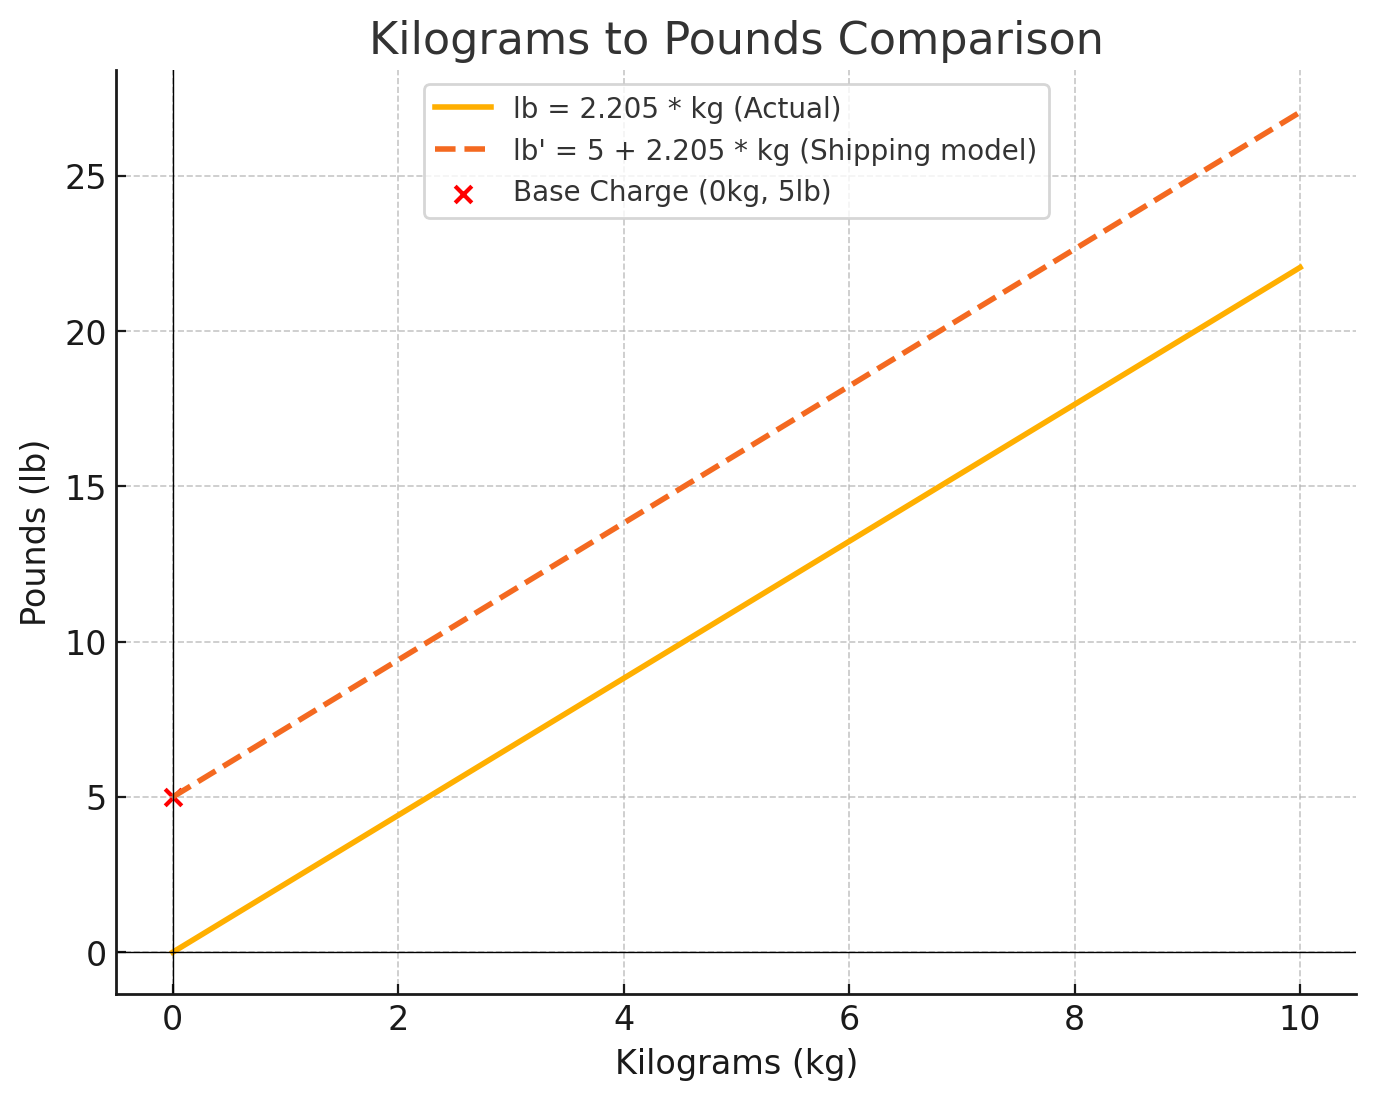
\includegraphics[width=0.45\linewidth]{Kilograms to Pounds Comparison.png}
\end{figure}

\subsection{Constant Function}
A constant function is a function \(f\) of the form \(f (x) = b\),  where \(b\) is a number.
\begin{figure}
\centering
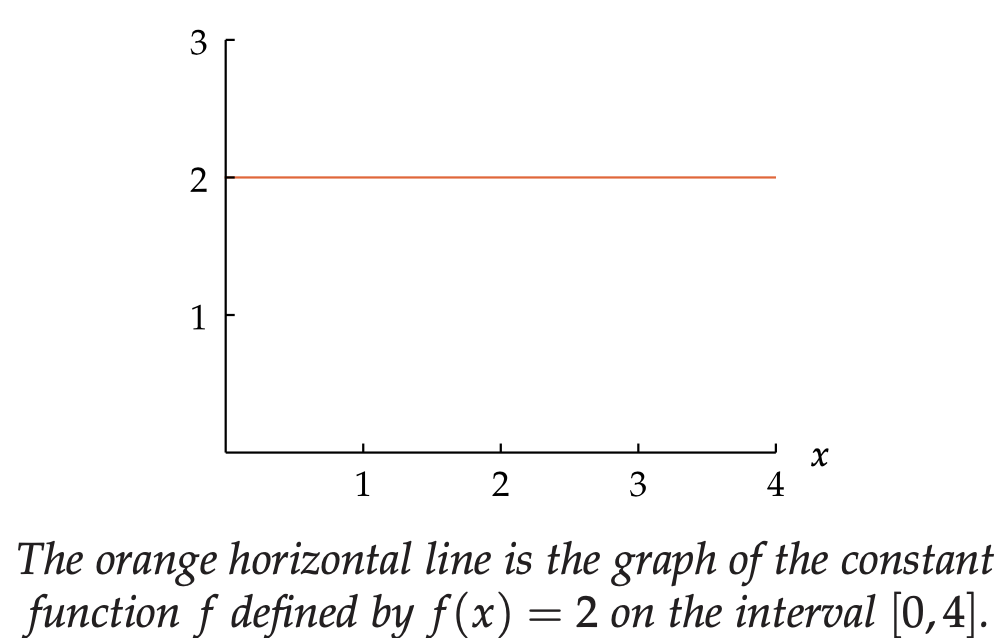
\includegraphics[width=0.6\linewidth]{constant.png}
\end{figure}

\subsection{Parallel Lines}
\begin{figure}
  \centering
  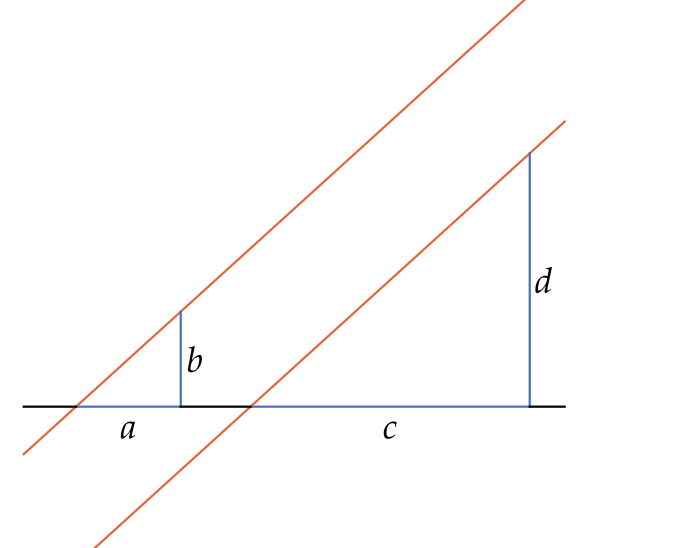
\includegraphics[scale=0.2]{parallel.png}
\end{figure}
As two lines are parallel, the corresponding angles are concurent and so two triangles are similar so
\[\frac{a}{c} = \frac{b}{d} \implies \frac{b}{a} = \frac{d}{c}  \]
it has same slope.

\subsection{Negative Slope}
\begin{figure}
  \centering
  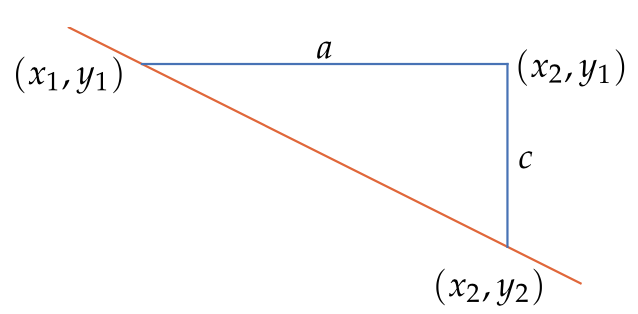
\includegraphics[scale=0.3]{negative-slope.png}
\end{figure}
As lengths are positive \(a = x_{2} - x_{1}\) and \(c = y_{1} - y_{2} \)
Slope  = \(\frac{y_{2} - y_{1}}{x_{2} - x_{1}} = -\frac{c}{a} \

\subsection{Perpendicular Lines}
\begin{figure}
  \centering
  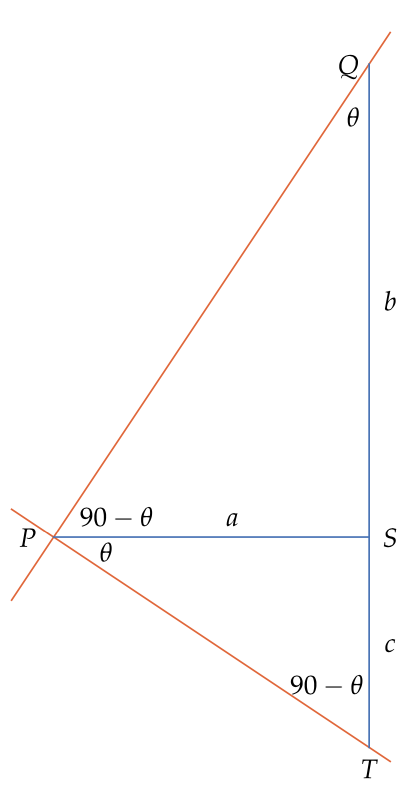
\includegraphics[width=0.5\linewidth]{perpendicular.png}
\end{figure}
\(\triangle PSQ \) and \( \triangle TSP \) are similar
\(\frac{QS}{SP} = \frac{PS}{ST} \implies \frac{b}{a} = \frac{a}{c} \
Multiplying by \(-\frac{c}{a} \implies \frac{b}{a} \cdot \left( - \frac{c}{a} \right) = -1  \

\subsection{Unequal Scales}
Angles are distorted by unequal scales on coordinate axes. In graphs with unequal scales on the two coordinate axes, angles are not accurately represented.
\begin{figure}
  \centering
  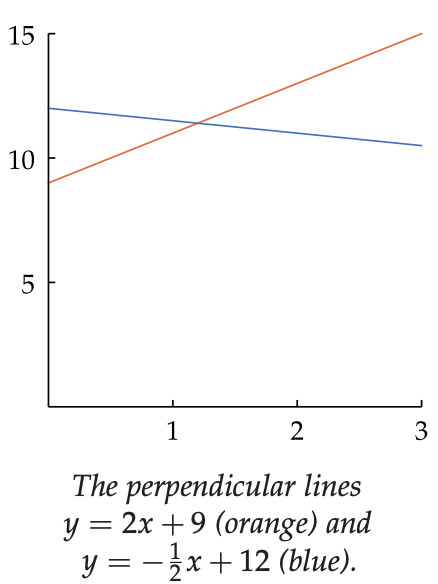
\includegraphics[scale=0.25]{unequal-scale.png}
\end{figure}

\section{Quadratic Functions and Conics}
\subsection{Conics}
\begin{figure}
  \begin{center}
    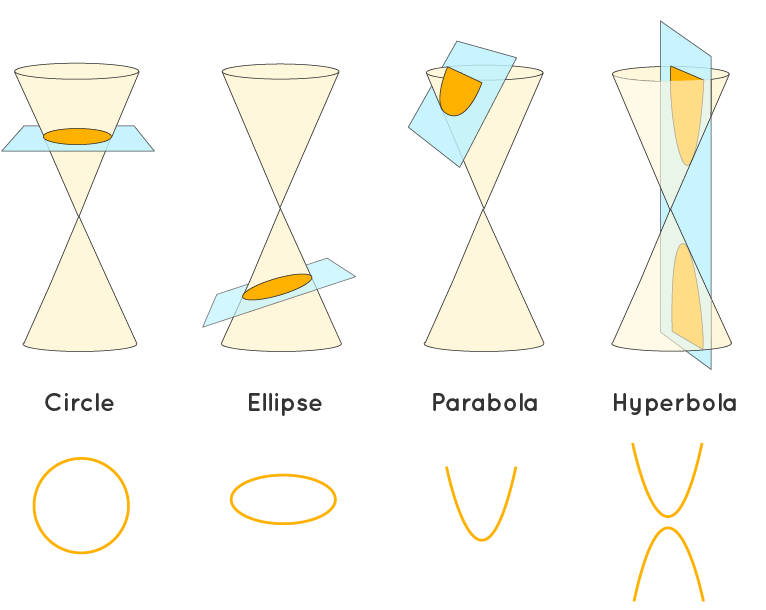
\includegraphics[scale = 0.3]{conic-section.png}
  \end{center}
\end{figure}

\subsection{Quadratic Function}
The function of the form
\[ax^{2} + bx + c = 0\]
where \(a,b,c\) are real numbers with \(a \neq 0\)
\begin{itemize}
    \item if \(b^{2} - 4ac < 0\), then equation have no real solutions
    \item if \(b^{2} - 4ac = 0\), then equation has one solution, \(x = -\frac{b}{2a}\)
    \item if \(b^{2} - 4ac  > 0\), then equation has two solutions \(x = \frac{-b \underset{-}{+}\sqrt{b^{2} - 4ac}}{2a}
\end{itemize}

\subsection{Parabola}
A \textbf{parabola} is the graph of a quadratic function. The \textbf{vertex} of the parabola is the where the line of symmetry of the parabola, intersects the parabola.
Suppose \(f\) is a quadratic function. Complete the square to write \(f\) in the form
\[ f(x) = a(x-h)^{2} + k \
\begin{itemize}
    \item If \(a > 0\) then \(f(x)\) attains its minimum value \(k\) when \(x=h\) and the graph of \(f\) is a parabola that opens upward.
    \item If \(a < 0 \) then \(f(x) \) its maximum value \(k\) when \(x=h\) and the graph of \(f\) is a parabola that opens downward
    \item The vertex of the graph is \(h,k\)
\end{itemize}

\subsubsection{Example}
\[f(x) = -3x^{2} + 12x - 8 \
\begin{enumerate}
  \item For what value of \(x\) does \(f (x) \) attain its maximum value?
  \item What is the maximum value of \(f (x)\)?
  \item Find the vertex
\end{enumerate}
Sol:
\[f(x) = -3x^{2} + 12x - 8 \implies -3(x^{2} - 4x + 4) + 4 \implies -3(x-2)^{2} + 4 \
\begin{enumerate}
\item \(x = 2\
\item \(f(x=2) = 4\
\item \( (2,4) \
\end{enumerate}

\begin{figure}
\centering
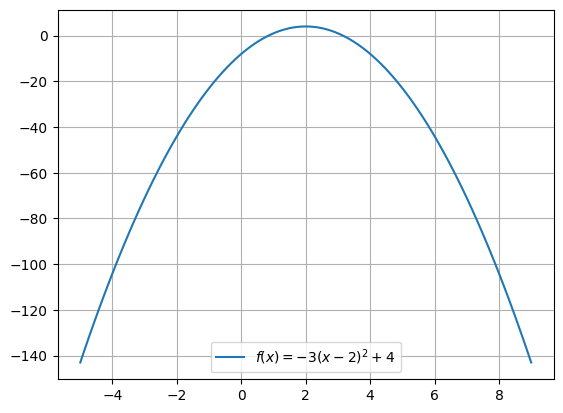
\includegraphics[scale=0.6]{parabola.png}
\end{figure}

\subsection{Distance Between Points}
\begin{figure}
\centering
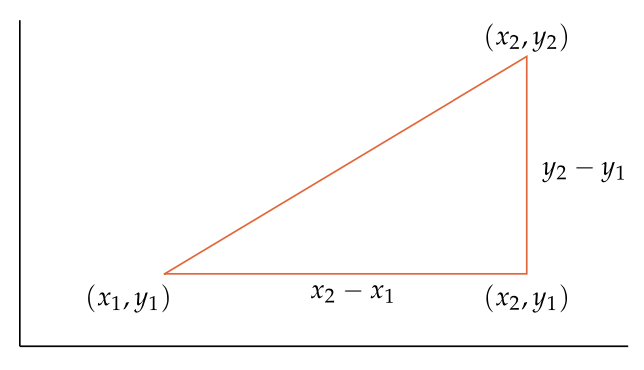
\includegraphics[scale=0.3]{distance-between-points.png}
\end{figure}
The distance between points \(x_{1}, y_{1}\) and \(x_{2}, y_{2}\) is given by
\[\sqrt{ \left(x_{2} - x_{1} \right)^{2}  + \left( y_{2} - y_{1} \right)^{2} }\]

\subsection{Circle}
The circle with center \(h,k\) and radius \(r\) is the set of the points \(x,y\) that satisfy the equation
\[\left(x-h\right)^{2} + \left(y-k\right)^{2} = r^{2}\]

\subsection{Ellipse}
\begin{figure}
\centering
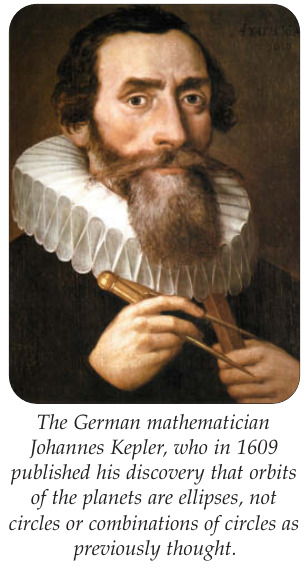
\includegraphics[scale=0.38]{ellipse0.png}
\end{figure}

Stretching the circle horizontally and/or vertically produces a curve called an \textbf{ellipse}.
\begin{figure}
\centering
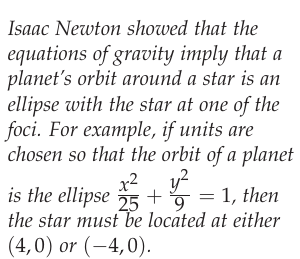
\includegraphics[scale=0.4]{ellipse1.png}
\end{figure}

\subsubsection{Example}
Equation of the circle is given by \(u^{2} + v^{2} = 1\).
By stretching \(x = 3u, y = 5v\),
Substituting for \(u,v\)
\[ \left( \frac{x}{3} \right)^{2} + \left(\frac{y}{5}\right)^{2} = 1 \

\subsubsection{Ellipse Equation}
\[\frac{x{2}}{a^{2}} + \frac{y^{2}}{b^{2}} = 1 \
The \textbf{foci} of an ellispe are two points with the property that the sum of the distances from the \textbf{foci} to any point on the ellipse is a constant independent of the point on the ellispe.

\begin{figure}
\centering
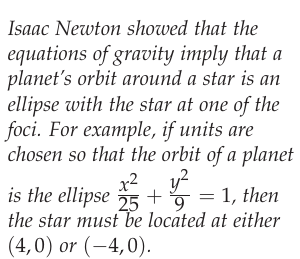
\includegraphics[scale=0.5]{ellipse1.png}
\end{figure}

\begin{figure}
\centering
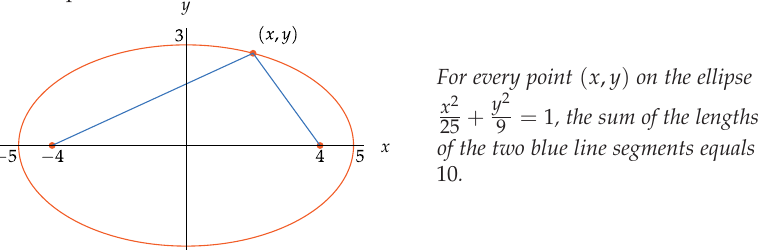
\includegraphics[scale=0.4]{foci.png}
\end{figure}

\subsection{Eccentricity of an Ellipse}
The \textbf{eccentricity} (\(e\)) of an ellipse is a measure of how much the ellipse deviates from being a circle. It is defined as
\[ e = \frac{c}{a} .
\qquad c^2 = a^2 - b^2, 
\qquad e = \sqrt{1 - \frac{b^2}{a^2}}\]
where:
\begin{itemize}
    \item \(c\) is the distance from the center to a focus.
    \item \(a\) is the length of the semi-major axis.
\end{itemize}
Additionally, the semi-minor axis \(b\) is related to \(a\) and \(c\) by:
\textbf{Key Points:}
\begin{itemize}
    \item If \(e = 0\), the ellipse is a circle.
    \item If \(0 < e < 1\), the ellipse is elongated, with greater elongation as \(e\) increases.
\end{itemize}

\subsection{Hyperbola}
The graph of the equation of the form
\[ \frac{y^2}{b^2} - \frac{x^2}{a^2} = 1 \
where \(a,b\) are non-zero numbers.
\begin{figure}
\centering
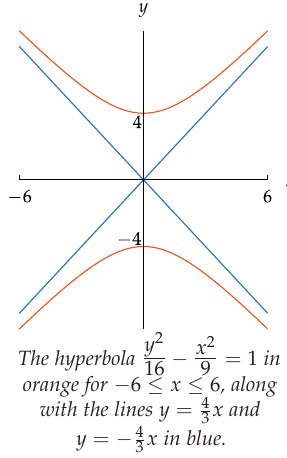
\includegraphics[scale=0.5]{pics/hyperbola2.png}
\end{figure}

The foci of a hyperbola are two points with the property that the difference of the distances from the foci to a point on the hyperbola is a constant independent of the point on the hyperbola.
\begin{figure}
\centering
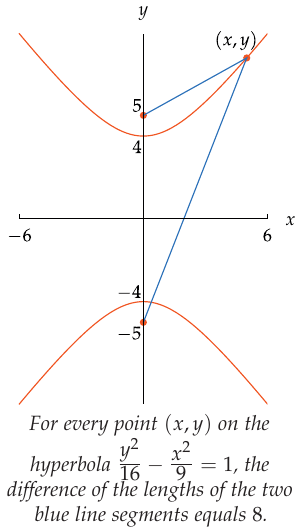
\includegraphics[scale=0.4]{pics/hyperbola3.png}
\end{figure}
\begin{figure}
\centering
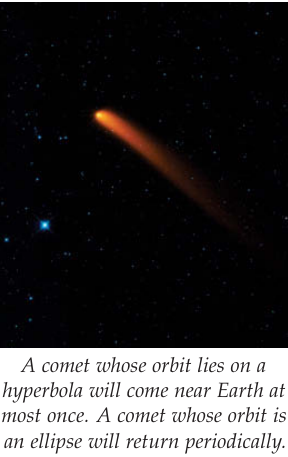
\includegraphics[scale=0.5]{pics/hyperbola1.png}
\end{figure}

\section{Exponents}
\subsection{Positive Integer Exponent}
If \(x\) is a real number and \(m\) is a positive integer, then \(x^{m}\) is defined to be the product with \(x\) appearing \(m\) times
\[x^{m} = \underset{x \;	ext{appears}\;	ext{m} \;	ext{times}}{\underbrace{x \cdot x \cdots x }}\]

\subsubsection{Properties}
Suppose \(x\) and \(y\) are numbers and \(m\) and \(n\) are positive integers. Then
\[x^{m}x^{n} = x^{m+n} \
\left(x^{m}\right)^{n} = x^{mn} \
x^{m}y^{m} = \left(xy\right)^{m}\]

\subsection{\(x^{0}\)}
If  \(x^{m}x^{n} = x^{m+n}\) then we can write \(x^{0}x^{n} = x^{0+n} = x^{n} \implies x^{0} = 1\;for\;	ext{x} \neq 0\]

\subsubsection{What is \(0^{0}\)}
\begin{itemize}
  \item The rule \( x^0 = 1 \) (for \( x \neq 0 \)) suggests that \( 0^0 \) should be \(1\).
  \item The rule \( 0^m = 0 \) (for \( m > 0 \)) suggests that \( 0^0 \) should be \(0\).
  \item Since these two rules contradict each other, \( 0^0 \) is left undefined in general mathematics.
  \item However, in combinatorics and programming, \( 0^0 \) is often defined as \(1\) for convenience.
\end{itemize}

\subsection{Negative Integer Exponents}
If \(x^{m}x^{n} = x^{m+n}\), if we take \(m = -n \), then
\[x^{m}x^{-m} = x^{0} = 1 \implies x^{m}x^{-m} = 1\]
We have to define \(x^{-m}\) to equal the multiplicative inverse of \(x^{m}\).
If \(x \neq 0\) and \(m\) is a positive integer, then \(x^{-m}\) is defined to multiplicative inverse of \(x^{m}\)
\[x^{-m} = \frac{1}{x^{m}}\]

\subsubsection{Exponents: Some Graphs}
\begin{figure}
\centering
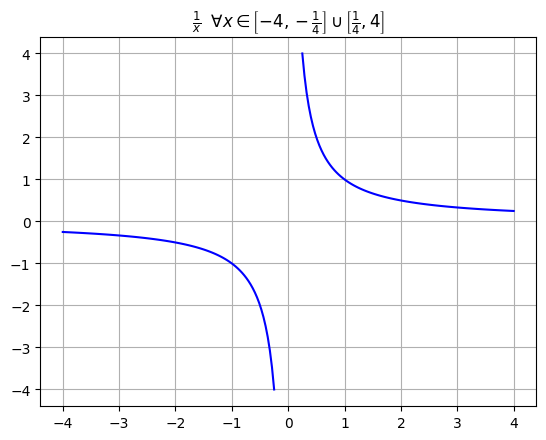
\includegraphics[scale=0.4]{pics/exponent-graph1.png}
\caption{graph of \(\frac{1}{x}\)}
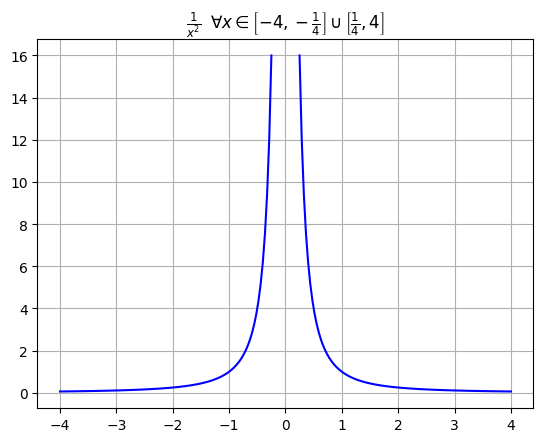
\includegraphics[scale=0.4]{pics/exponent-graph2.png}
\caption{graph of \(\frac{1}{x^{2}}\)}
\end{figure}

\subsubsection{Graph of Negative Integer Exponents}
if \(m\) is  a positive integer then
\begin{itemize}
  \item \(\frac{1}{x^{m}}\) behaves like \(\frac{1}{x}\) if \(m\) is odd
  \item \(\frac{1}{x^{m}}\) behaves like \(\frac{1}{x^{2}}\) if \(m\) is even
  \item Larger values of \(m\) correspond to functions whose graphs get closer to the x-axis more rapidly for large values of \(x\) and closer to the vertical axis more rapidly for values of \(x\) near 0
\end{itemize}

\subsection{Roots}
\subsubsection{\(m^{th}\) root}
If \(m\) is a positive integer and \(x\) is a real number, then \(x^{1/m}\) is defined to be the real number satisfying the equation
\[\left(x^{1/m}\right)^{m} = x \
subject to the following conditions:
\begin{itemize}
\item  If \(x < 0\) and \(m\) is an even integer, then \(x^{1/m} \)is undefined
\item If \(x > 0\) and \(m\) is an even integer, then \(x^{1/m} \)is chosen to be the \textit{\textcolor{red}{positive number}} satisfying the equation above
\end{itemize}
The number \(x^{1/m}\) is called the \textbf{\(m^{th}\)} root of \(x\).

\subsubsection{Example}
\begin{itemize}
  \item \(8^{1/3}\) and \(-8^{1/3}\)
  \item \(9^{1/2}\) and \(-9^{1/2}\)
\end{itemize}
Solution:
\begin{enumerate}
  \item \( \left(8^{1/3}\right)^{3} = 8 \implies 2 \
  \item \( \left(-8^{1/3}\right)^{3} = -8 \implies -2 \). There is no other number other than \(-2\)
  \item \( \left( 9^{1/2} \right)^{2} = -3 \; or \;3\). But as per the rule, we have to choose positive possibility, that is \(3\
  \item \( \left( -9^{1/2} \right)^{2} \). No number real number exists so no solution
\end{enumerate}

\subsection{Rational Exponents}
Suppose \(\frac{n}{m}\) is a fraction in reduced form, where \(n\) and \(m\) are integers and \(m > 0\). Then, whenever it makes sense,
\[ x^{\frac{n}{m}} = \Bigl(x^{\frac{1}{m}}\Bigr)^n. \
\textbf{Note:} For the expression \(x^{\frac{1}{m}}\) to be defined, additional conditions on \(x\) may be required (for example, if \(m\) is even, then typically \(x \ge 0\)).

\subsection{Algebra of Exponents}
Let \(p, q\) be rational numbers and \(x, y\) be positive numbers. Then the following rules hold:
\begin{itemize}
  \item \(x^p \cdot x^q = x^{\,p+q}
  \item \(x^p \cdot y^p = (xy)^p
  \item \((x^p)^q = x^{\,pq}
  \item \(x^0 = 1
  \item \(x^{-p} = \dfrac{1}{x^p}
  \item \(\dfrac{x^p}{x^q} = x^{\,p-q}
  \item \(\left(\dfrac{x}{y}\right)^p = \dfrac{x^p}{y^p}
\end{itemize}

\section{Polynomials}
\subsection{Polynomial Definition}
A polynomial is a function \( p \) such that
\[ p(x) = a_0 + a_1 x + a_2 x^2 + \cdots + a_n x^n, \
where \( n \) is a nonnegative integer and \( a_0, a_1, a_2, \dots, a_n \) are numbers.

\subsection{Degree of a Polynomial}
Suppose \( p \) is a polynomial defined by
\[ p(x) = a_0 + a_1 x + a_2 x^2 + \cdots + a_n x^n. \
If \( a_n \neq 0 \), then we say that \( p \) has degree \( n \). The degree of \( p \) is denoted by \(\deg p\).

\subsection{Polynomial Graphs}
\begin{figure}
\centering
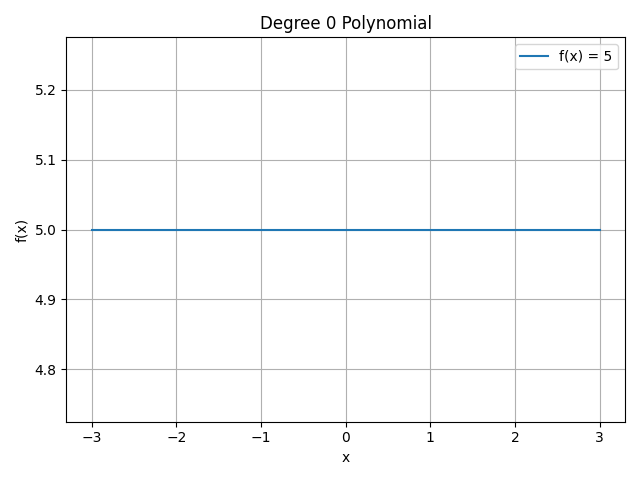
\includegraphics[width=0.45\linewidth]{pics/polynomial_degree_0.png}
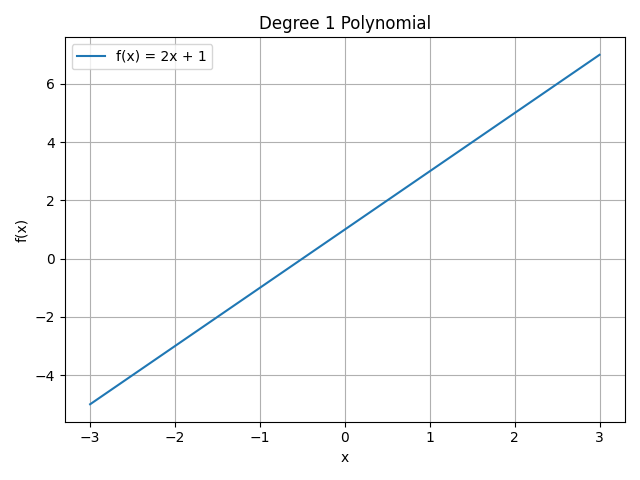
\includegraphics[width=0.45\linewidth]{pics/polynomial_degree_1.png}
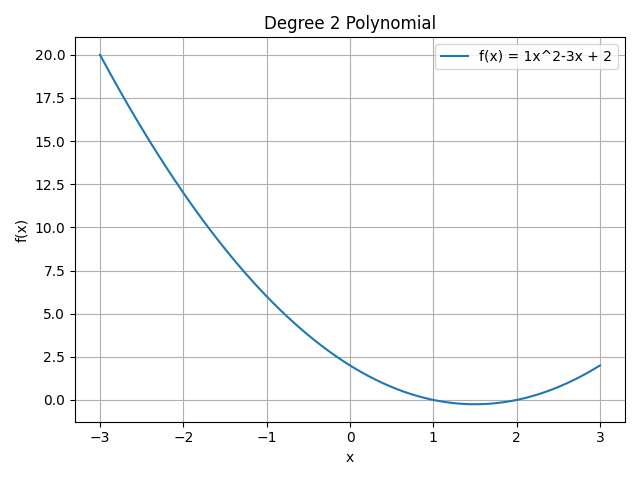
\includegraphics[width=0.45\linewidth]{pics/polynomial_degree_2.png}
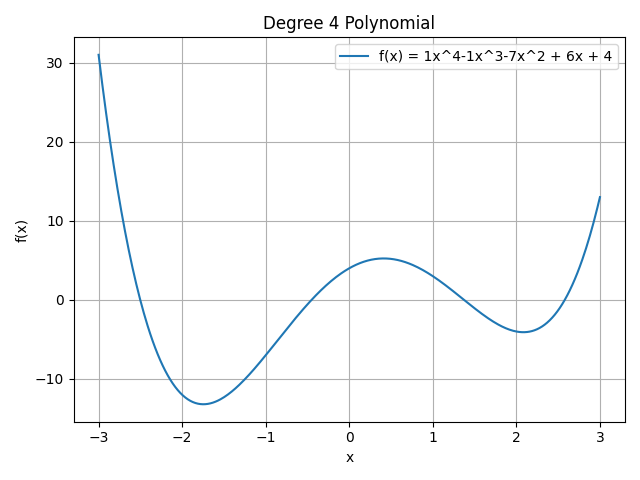
\includegraphics[width=0.45\linewidth]{pics/polynomial_degree_4.png}
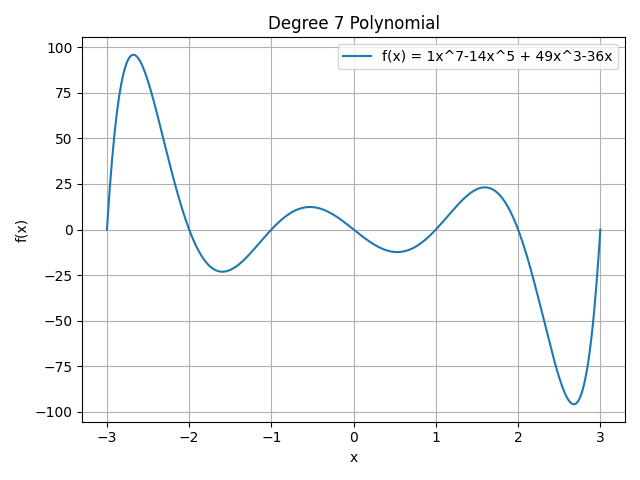
\includegraphics[width=0.45\linewidth]{pics/polynomial_degree_7.png}
\end{figure}

\subsection{The Algebra of Polynomials}
Two functions can be added, subtracted, or multiplied, producing another function. Specifically, if \(p\) and \(q\) are functions, then the functions
\[ p+q,\quad p-q,\quad \text{and} \quad pq \
are defined by
\[ (p+q)(x) = p(x) + q(x), \
\[ (p-q)(x) = p(x) - q(x), \
\[ (pq)(x) = p(x) \, q(x). \

\subsection{Degree of the Sum and Difference of Two Polynomials}
If \(p\) and \(q\) are nonzero polynomials, then
\[ \deg(p+q) \leq \max\{\deg p,\, \deg q\}, \
and
\[ \deg(p-q) \leq \max\{\deg p,\, \deg q\}. \

\subsection{Degree of the Product of Two Polynomials}
If \(p\) and \(q\) are nonzero polynomials, then
\[ \deg(pq) = \deg p + \deg q. \

\subsection{Example: Polynomials \(p\) and \(q\)}
Suppose \(p\) and \(q\) are polynomials defined by
\[ p(x) = 2 - 3x^2 \quad \text{and} \quad q(x) = 4x + 7x^5. \
Answer the following:
\begin{enumerate}
    \item What is \(\deg p\)?
    \item What is \(\deg q\)?
    \item Find a formula for \(pq\).
    \item What is \(\deg(pq)\)?
\end{enumerate}
Solution:
\begin{enumerate}
    \item Since \(p(x) = 2 - 3x^2\) has the highest power \(x^2\), we have \(\deg p = 2\).
    \item For \(q(x) = 4x + 7x^5\), the highest power is \(x^5\), so \(\deg q = 5\).
    \item The product \(pq\) is computed as follows:
    \[ pq = (2-3x^2)(4x+7x^5) = 2\cdot 4x + 2\cdot 7x^5 - 3x^2\cdot 4x - 3x^2\cdot 7x^5, \
    which simplifies to:
    \[ pq = 8x - 12x^3 + 14x^5 - 21x^7. \
    \item The highest power in \(pq\) is \(x^7\), so \(\deg(pq) = 7\).
\end{enumerate}

\subsection{Zeros/Roots of a Function}
A number \(t\) is called a zero of a function \(p\) if
\[ p(t) = 0. \

\subsection{Closed-Form Expression}
A closed-form expression is an explicit formula that can be written using a finite number of standard operations and functions (e.g., addition, multiplication, exponentiation, logarithms, trigonometric functions). It does not involve infinite series, integrals, or iterative processes.
\textbf{Example:} The quadratic formula,
\[ x = \frac{-b \pm \sqrt{b^2-4ac}}{2a}, \
is a closed-form expression.

\subsection{Zeros of Higher–Degree Polynomials}
\begin{itemize}
  \item The quadratic formula gives exact zeros for degree–2 polynomials.
  \item Although formulas exist for cubics and quartics, they are rarely used.
  \item No closed-form formula exists for polynomials of degree 5 or higher.
  \item Numerical methods can approximate zeros for any polynomial.
  \item \textbf{Example:} For
  \[ p(x)=x^5-5x^4-6x^3+17x^2+4x-7, \
  approximate zeros are:
  \[ -1.80,\; -0.73,\; 0.63,\; 1.48,\; 5.56. \
\end{itemize}

\subsubsection{Zeros on graph}
\begin{figure}
\centering
\includegraphics[scale=0.23]{pics/zeros.png}
\end{figure}
\begin{figure}
\centering
\includegraphics[scale=0.3]{pics/no-real-zeros.png}
\caption{The function \(x^{2}+1\) has no real zeros}
\end{figure}

\subsection{Factor of a Polynomial}
Suppose \(p\) is a polynomial and \(t\) is a real number. Then \(x-t\) is called a \emph{factor} of \(p(x)\) if there exists a polynomial \(G(x)\) such that
\[ p(x) = (x-t)\,G(x) \
for every real number \(x\).

\subsection{Example: Factors and Zeros of a Polynomial}
Let
\[ p(x) = (x-2)(x-5)(x^2+1). \
\begin{enumerate}[(a)]
  \item Explain why \(x-2\) is a factor of \(p(x)\).
  \item Explain why \(x-5\) is a factor of \(p(x)\).
  \item Show that \(2\) and \(5\) are zeros of \(p\).
  \item Show that \(p\) has no (real) zeros except \(2\) and \(5\).
\end{enumerate}
Solution:
\begin{enumerate}[(a)]
  \item The polynomial is given in factored form as \((x-2)(x-5)(x^2+1)\). Since \((x-2)\) appears as one of the factors, it is a factor of \(p(x)\).
  \item Similarly, \((x-5)\) appears explicitly in the factorization, so it is a factor of \(p(x)\).
  \item To show that \(2\) and \(5\) are zeros, substitute:
    \[ p(2) = (2-2)(2-5)(2^2+1) = 0\cdot(-3)\cdot5 = 0, \
    \[ p(5) = (5-2)(5-5)(5^2+1) = 3\cdot0\cdot26 = 0. \
    Thus, \(p(2)=0\) and \(p(5)=0\).
  \item The factor \(x^2+1\) yields \(x^2=-1\), which has no real solutions. Hence, aside from the zeros from \((x-2)\) and \((x-5)\), there are no other real zeros.
\end{enumerate}

\subsection{Zeros and Factors of a Polynomial}
Suppose \(p\) is a polynomial and \(t\) is a real number. Then \(t\) is a zero of \(p\) if and only if \(x-t\) is a factor of \(p(x)\).

\subsection{Number of Zeros of a Polynomial}
A nonzero polynomial \(p(x)\) of degree \(n\) has at most \(n\) zeros.
A polynomial of degree 15 has at most 15 zeros. This is because each (real) zero \(t_j\) of a polynomial \(p\) corresponds to a factor \((x-t_j)\) in a factorization of the form
\[ p(x) = (x-t_1)(x-t_2)\cdots(x-t_m) \, G(x), \
where \(G(x)\) is a polynomial with no (real) zeros. If \(p(x)\) had more than 15 zeros, then the right-hand side would represent a polynomial of degree higher than 15, contradicting the fact that \(p\) is of degree 15.

\subsection{Behavior of a Polynomial Near \(\pm\infty\)}
\begin{itemize}
  \item \textbf{\(x\) near \(+\infty\):} \(x\) is very large.
  \item \textbf{\(x\) near \(-\infty\):} \(x\) is very negative (i.e., \(|x|\) is very large).
  \item Our goal is to determine whether a polynomial \(p(x)\) is positive or negative in these extremes.
\end{itemize}
\begin{figure}
\centering
\includegraphics[scale=0.2]{pics/at-infty.png}
\end{figure}
To analyze the behavior as \(x\to\pm\infty\), factor out the highest degree term.
If \(c\,x^n\) is the highest degree term in \(p(x)\), then for very large \(|x|\), \(p(x)\) behaves like \(c\,x^n\).

\subsection{Zero in an Interval}
\subsubsection{Intermediate Value Theorem}
Suppose \(p\) is a polynomial and \(a, b \in \mathbb{R}\) with \(a < b\). If \(p(a)\) and \(p(b)\) have opposite signs, then there exists a number \(c \in (a, b)\) such that \(p(c)=0\).

\subsection{Example 7: Zero in an Interval}
Let
\[ p(x) = x^5 + x^2 - 1. \
Explain why \(p\) has a zero in the interval \((0,1)\).
Solution:
Evaluate the polynomial at the endpoints:
\[ p(0) = 0^5 + 0^2 - 1 = -1 \quad \text{and} \quad p(1) = 1^5 + 1^2 - 1 = 1. \
Since \(p(0) < 0\) and \(p(1) > 0\), by the Intermediate Value Theorem, there exists a \(c \in (0,1)\) such that \(p(c)=0\).

\subsection{Zeros for Polynomials with Odd Degree}
Every polynomial with odd degree has at least one real zero.
For a polynomial \(p(x)\) of odd degree, as \(x \to -\infty\), \(p(x)\) tends to \(-\infty\) (or \(+\infty\)) and as \(x \to \infty\), \(p(x)\) tends to \(+\infty\) (or \(-\infty\)).
By the Intermediate Value Theorem, since \(p(x)\) changes sign, there exists at least one real number \(c\) such that \(p(c)=0\).

\section{Rational Function}
\subsection{Definition}
A \emph{rational function} is a function \(r\) defined by
\[ r(x) = \frac{p(x)}{q(x)}, \
where \(p(x)\) and \(q(x)\) are polynomials, with \(q(x) \neq 0\).

\subsection{Domain of a Rational Function & Example for \(r(x)\)}
The domain of a rational function
\[ \frac{p(x)}{q(x)} \
is the set of all real numbers where the expression makes sense. Since division by 0 is undefined, we exclude all zeros of \(q(x)\).

\subsubsection{Example}
\[r(x)=\frac{3x^5+x^4-6x^3-2}{x^2-9}\]
Factor the denominator:
\[ x^2-9=(x-3)(x+3). \
Thus, \(r(x)\) is undefined at \(x=3\) and \(x=-3\). Hence, its domain is
\[ \{x\in\mathbb{R}: x\neq 3 \text{ and } x\neq -3\}. \

\subsubsection{Example}
\[s(x)=\frac{x^3-6x+5}{x^4+9}\]
The denominator \(x^4+9\) is always positive (since \(x^4\ge 0\) and \(9>0\)). Therefore, \(s(x)\) is defined for every real number.
Domain of \(s(x)\) :
\( \mathbb{R} \

\subsection{Advantages of Mixed Representation}
Expressing a rational function as a polynomial plus a proper rational function (one where the numerator's degree is less than the denominator's) is analogous to writing an improper fraction as an integer plus a proper fraction.
\begin{itemize}
  \item \textbf{Simplification:} It makes further operations (such as integration, differentiation, and partial fraction decomposition) easier.
  \item \textbf{Asymptotic Insight:} The polynomial part reveals the behavior of the function as \(x\to\pm\infty\), while the proper fraction (the remainder) tends to zero for large \(|x|\).
  \item \textbf{Clarity:} It separates the "whole" part from the "fractional" part, making the function's structure more transparent.
\end{itemize}

\subsection{Mixed Rational Function Representation}
Express
\[ \frac{x^5 + 6x^3 + 11x + 7}{x^2+4} \
in the form
\[ G(x) + \frac{ax+b}{x^2+4}, \
where \(G(x)\) is a polynomial and \(a, b\) are constants.

\subsection{Procedure for Dividing Polynomials}
\begin{enumerate}
  \item \textbf{Rewrite:} Express the highest-degree term in the numerator as a single term times the denominator, plus the necessary adjustment.
  \item \textbf{Simplify:} Use the rewritten numerator to simplify the quotient.
  \item \textbf{Iterate:} Repeat steps (1) and (2) on the remaining rational function until the degree of the numerator is less than the degree of the denominator or the numerator becomes 0.
\end{enumerate}

\subsection{Mixed Representation Example}
Express
\[ \frac{x^5+6x^3+11x+7}{x^2+4} \
in the form
\[ G(x)+\frac{ax+b}{x^2+4}, \
where \(G(x)\) is a polynomial and \(a, b\) are constants.
\subsubsection{Step 1: Eliminate the \(x^5\) Term}
Notice that
\[ x^5=x^3(x^2+4)-4x^3. \
Therefore,
\[
\begin{aligned}
  x^5+6x^3 &= x^3(x^2+4)-4x^3+6x^3\\[1mm]
           &= x^3(x^2+4)+2x^3.
\end{aligned}
\]
So we can write:
\[ \frac{x^5+6x^3+11x+7}{x^2+4}=x^3+\frac{2x^3+11x+7}{x^2+4}. \

\subsubsection{Step 2: Eliminate the \(2x^3\) Term}
Write
\[ 2x^3=2x(x^2+4)-8x. \
Then,
\[
\begin{aligned}
  2x^3+11x+7 &= 2x(x^2+4)-8x+11x+7\\[1mm]
              &= 2x(x^2+4)+(3x+7).
\end{aligned}
\]
Thus,
\[ \frac{2x^3+11x+7}{x^2+4}=2x+\frac{3x+7}{x^2+4}. \

\subsubsection{Final Mixed Representation}
Combining the steps, we have:
\[ \frac{x^5+6x^3+11x+7}{x^2+4}=x^3+2x+\frac{3x+7}{x^2+4}. \

\subsection{Division Algorithm for Polynomials}
If \(p(x)\) and \(q(x)\) are polynomials with \(q(x) \neq 0\), then there exist unique polynomials \(G(x)\) and \(R(x)\) such that
\[ \frac{p(x)}{q(x)} = G(x) + \frac{R(x)}{q(x)}, \
where either \(R(x)=0\) or \(\deg R < \deg q\). Equivalently, we can write
\[ p(x)=q(x)G(x)+R(x). \

\subsection{Division by \(x-t\) and Zeros of a Polynomial}
Fix a real number \(t\) and let \(q(x)=x-t\). Since \(\deg q=1\), the remainder \(R(x)\) is a constant \(c\)(Because degree \(R < \)degree \(q\)). Thus, there exist a polynomial \(G(x)\) and a constant \(c\) such that
\[ p(x) = (x-t)G(x) + c. \
Evaluating at \(x=t\) yields \(p(t)=c\), so we can rewrite this as
\[ p(x) = (x-t)G(x) + p(t). \
\(t\) is a zero of \(p\) if and only if \(p(t)=0\), which happens precisely when
\[ p(x)=(x-t)G(x). \

\subsection{Behavior of a Rational Function Near \(\pm\infty\)}
To determine the behavior of a rational function as \(x\to\pm\infty\), factor out the highest power of \(x\) in the numerator and the denominator.
Consider
\[ r(x)=\frac{9x^5-2x^3+1}{x^8+x+1}. \
The highest degree in the numerator is \(x^5\) and in the denominator is \(x^8\). Factoring these out yields:
\[ r(x) \sim \frac{9x^5}{x^8}=\frac{9}{x^3}. \
As \(|x|\) becomes very large:
\begin{itemize}
  \item \(r(x)\to 0\) as \(x\to\infty\) (approaching \(0^+\)).
  \item \(r(x)\to 0\) as \(x\to-\infty\) (approaching \(0^-\)).
\end{itemize}

\subsection{Asymptote of a Rational Function}
A line is an asymptote of a graph if the graph becomes and stays arbitrarily close to the line as \(x\) tends to \(\pm\infty\).
Consider
\[ r(x)=\frac{3x^6-9x^4+6}{2x^6+4x+3}. \
Both the numerator and the denominator are degree 6. Therefore, the horizontal asymptote is the ratio of the leading coefficients:
\[ y=\frac{3}{2}. \
\begin{figure}
\centering
\includegraphics[scale=0.2]{pics/asymptote1.png}
\end{figure}

\subsubsection{Example}
\[ r(x) = \frac{4x^{10}-2x^3+3x+15}{2x^6+x^5+1} \
Solution:
\[ \frac{4x^{10}}{2x^6} = 2x^4. \
Thus, as \(|x|\to\infty\), \(r(x)\) behaves like \(x^{4}\). That is, \(r(x)\) is very large and positive when \( x \to \infty\) and \( x \to -\infty\).

\chapter{Exponential Functions, Logarithms and e}
\author{Nithin}

\section{Bacterial Growth on the Human Body}
\begin{itemize}
  \item Our skin (and other areas like the mouth, nose, and intestines) hosts hundreds of thousands of microscopic organisms.
  \item In fact, bacterial cells in our body outnumber our own cells.
  \item While some bacteria can cause illness, many are essential for our health.
  \item Bacteria reproduce through binary fission—each cell splits into two.
  \item Under ideal conditions, a single bacterium doubling every hour can lead to over 1,000 cells in 10 hours and more than 16 million in 24 hours.
\end{itemize}

\subsection{Bacterial Growth Over Time}
\begin{table}[ht]
  \centering
  \begin{tabular}{c|ccccccccccc}
    \textbf{Hour} & 0 & 1 & 2 & 3 & 4 & 5 & 6 & 7 & 8 & 9 & 10 \\ \hline
    \textbf{Bacteria} & 1 & 2 & 4 & 8 & 16 & 32 & 64 & 128 & 256 & 512 & 1024 \\
  \end{tabular}
  \caption{Bacterial cell count doubling every hour.}
\end{table}

\section{Population Growth in India}
\begin{itemize}
  \item India is the second most populous country, with about 1.39 billion people in 2021.
  \item Its population grows at an annual rate of roughly 1.2\%.
  \item If this trend continues, India's population is projected to exceed China’s by 2027.
  \item While rapid population increases are often described as "exponential," in mathematics the term has a very precise meaning.
\end{itemize}

\section{Defining Exponential Growth}
\begin{itemize}
  \item \textbf{Percentage Change:}
  \begin{itemize}
    \item refers to a change based on a percent of the original amount
  \end{itemize}
  \item \textbf{Exponential Growth:}
    \begin{itemize}
      \item refers to an increase based on a constant multiplicative rate of change over equal increments of time, that is, a percent increase of the original amount over time.
      \item For example, if a quantity doubles each period, that is a 100\% increase per period.
    \end{itemize}
  \item \textbf{Linear Growth:}
    \begin{itemize}
      \item The original value increases by a fixed \textbf{amount} (additive rate) over equal time intervals.
    \end{itemize}
    \item \textbf{Exponent Decay:}
    \begin{itemize}
      \item refers to a decrease based on a constant multiplicative rate of change over equal increments of time, that is, a percent decrease of the original amount over time.
    \end{itemize}
\end{itemize}

\section{Exponential Function and Its Behavior}
Suppose \(b>0\) with \(b\neq 1\). Then the \emph{exponential function} with base \(b\) is defined by
\[ f(x)=b^x. \]
For example, if \(b=2\), then \(f(x)=2^x\). (Note that \(2^x\) is different from \(x^2\).)

\subsection{Behavior (for \(b>1\))}
\begin{itemize}
  \item \textbf{Domain:} All real numbers, \(\mathbb{R}\).
  \item \textbf{Range:} All positive numbers, \((0,\infty)\).
  \item \(f(x)=b^x\) is an \emph{increasing} function.
  \item \(b^x\) becomes very large as \(x\) increases.
  \item \(b^x\) approaches \(0\) as \(x\) becomes very negative.
\end{itemize}

\section{Comparing Exponential and Linear Growth}
\begin{table}[ht]
  \centering
  \begin{tabular}{c|c|c}
    \(x\) & \(f(x)=2^x\) & \(g(x)=2x\) \\ \hline
    0 & 1 & 0 \\
    1 & 2 & 2 \\
    2 & 4 & 4 \\
    3 & 8 & 6 \\
    4 & 16 & 8 \\
  \end{tabular}
  \caption{Exponential vs. Linear Growth.}
\end{table}
\begin{itemize}
  \item Linear growth (e.g., \(g(x)=2x\)) increases by a constant amount (2) for each increase in \(x\), that is, it is adding or subtracting a constant value. A constant amount \( \rightarrow \) linear growth or additive growth.
  \item Exponential growth (e.g., \(f(x)=2^x\)) increases by a constant factor (2) for each increase in \(x\), that is, it is multiplying or dividing by a constant value. A constant factor \( \rightarrow \) exponential growth or multiplicative growth.
\end{itemize}

\section{Example: The Function \(f(x)=2^x\)}
\begin{table}[ht]
  \centering
  \begin{tabular}{|c|c|c|c|c|c|c|c|}
    \hline
    \(x\)      & -3 & -2 & -1 & 0 & 1 & 2 & 3 \\ \hline
    \(2^x\) & \(2^{-3}=\frac{1}{8}\) & \(2^{-2}=\frac{1}{4}\) & \(2^{-1}=\frac{1}{2}\) & \(2^0=1\) & \(2^1=2\) & \(2^2=4\) & \(2^3=8\) \\ \hline
  \end{tabular}
  \caption{Exponential values of \(2^x\) for \(x=-3,\dots,3\).}
\end{table}
\textbf{Observation:} As \(x\) increases by 1, the output of \(2^x\) doubles, clearly illustrating exponential growth.

\section{Algebraic Properties of Exponents}
Let \(a, b > 0\) and \(x, y \in \mathbb{R}\). Then:
\begin{itemize}
  \item \(b^x \cdot b^y = b^{x+y}\)
  \item \((b^x)^y = b^{xy}\)
  \item \(a^x \cdot b^x = (ab)^x\)
  \item \(b^0 = 1\)
  \item \(b^{-x} = \dfrac{1}{b^x}\)
  \item \(\dfrac{b^x}{b^y} = b^{x-y}\)
  \item \(\dfrac{a^x}{b^x} = \Bigl(\dfrac{a}{b}\Bigr)^x\)
\end{itemize}

\subsection{Exponent Graph}
\begin{figure}
\centering
\includegraphics[scale=0.3]{pics/exp-vs-poly1.png}
\includegraphics[scale=0.2]{pics/exp-vs-poly2.png}
\end{figure}

\section{Logarithm}
Suppose \(b\) and \(y\) are positive numbers with \(b\neq 1\).
\begin{itemize}
  \item The logarithm base \(b\) of \(y\), denoted \(\log_b y\), is defined as the unique number \(x\) such that
  \[ b^x = y. \]
  \item  Short Version
  \[ \log_b y = x \quad \text{means} \quad b^x = y. \]
\end{itemize}

\subsection{Logarithm of 1 and the Base}
Let \(b>0\) with \(b\neq 1\). Then:
\begin{itemize}
  \item \(\log_b 1 = 0\) because \(b^0 = 1\),
  \item \(\log_b b = 1\) because \(b^1 = b\).
\end{itemize}

\subsection{Logarithm as an Inverse Function}
Suppose \(b\) is a positive number with \(b \neq 1\) and the exponential function \(f\) is defined by
\[ f(x) = b^x. \]
Then the inverse function \(f^{-1}\) is given by
\[ f^{-1}(y) = \log_b y. \]

\subsection{Inverse Properties of Logarithms - Summary}
\begin{itemize}
  \item \textbf{Inverse Relationship:}
    \begin{itemize}
      \item \(\log_b x\) is the inverse of \(b^x\).
      \item Flipping the graph of \(b^x\) across the line \(y=x\) yields the graph of \(\log_b x\).
    \end{itemize}
  \item \textbf{Monotonicity:}
    \begin{itemize}
      \item For \(b>1\), \(b^x\) is increasing, so \(\log_b x\) is also increasing.
    \end{itemize}
  \item \textbf{Key Equations:}
    \begin{itemize}
      \item \(b^{\log_b y} = y\)
      \item \(\log_b (b^x) = x\)
    \end{itemize}
  \item \textbf{Function-Inverse Properties:}
    \begin{itemize}
      \item These can be written as \((f \circ f^{-1})(y) = y\) and \((f^{-1} \circ f)(x) = x\).
    \end{itemize}
  \item \textbf{Understanding:}
    \begin{itemize}
      \item These properties are fundamental to the relationship between exponential and logarithmic functions.
    \end{itemize}
\end{itemize}

\subsection{Logarithm of a Power}
If \(b\) and \(y\) are positive numbers, with \(b \neq 1\), and \(t\) is a real number, then
\[ \log_b\left(y^t\right) = t \log_b y. \]

\section{Radioactive Decay}
If a radioactive isotope has half-life \(h\), then the function modeling the number of atoms in a sample of this isotope is
\[ a(t) = a_{0}2^{-t/h}\]
where \(a_{0}\) is the number of atoms of the isotope in the sample at time \(0\).

\section{Exponential Growth}
\subsection{A story}
A mathematician in ancient India invented the game of chess. Filled with gratitude for the remarkable entertainment of this game, the king offered themathematician anything he wanted. The king expected the mathematician to ask for rare jewels or a majestic palace. But the mathematician asked only that he be given one grain of rice for the first square on a chessboard, plus two grains of rice for the next square, plus four grains for the next square, and so on, doubling the amount for each square, until the 64th square on an 8-by-8 chessboard had been reached. The king was pleasantly surprised that the mathematician had asked for such a modest reward. A bag of rice was opened, and first 1 grain was set aside, then 2, then 4, then 8, and so on. As the eighth square was reached, 128 grains of rice were counted out. The king was secretly delighted to be paying such a small reward and also wondering at the foolishness of the mathematician.

As the 16th square was reached, 32,768 grains of rice were counted out—this was a small part of a bag of rice. But the 21st square required a full bag of rice, and the 24th square required eight bags of rice. This was more than the king had expected. However, it was a trivial amount because the royal granary contained about 200,000 bags of rice to feed the kingdom during the coming winter. As the 31st square was reached, over a thousand bags of rice were required and were delivered from the royal granary. Now the king was worried. By the 37th square, the royal granary was two-thirds empty. The 38th square would have required more bags of rice than were left. The king then stopped the process and ordered that the mathematician's head be chopped off as a warning about the greed induced by exponential growth.

\subsection{Mathematical analysis}
\begin{itemize}
  \item \(64^{th}\) square requires \( 2^{63} \) grains \(\approx\) \(2^{3}* (2^{10})^{6} = 8*(10^{3})^{6} = 8*10^{18} \approx 10^{19} \)
  \item if one large bag = \(10^{6} \) grains of rice , then total bags = \(10^{19}/10^{6} \)
  \item In 2025 India's population is \(\approx 1 * 10^{9} \)
\end{itemize}

A function \(f\) is said to have \textbf{exponential growth} if \(f(x) = cb^{kx} \) where
\(c\) and \(k\) are positive numbers and \(b > 1\).
\begin{itemize}
  \item \(f(x) > p(x)\)  where \(f\) is exponenetial and \(p\) is polynomial for sufficiently large \(x\)
  \item \(2^{x} > x^{1000} \)  \(\forall \;	kWidget x > 13747 \)
  \item A function \(f\) has exponential growth if and only if the graph of \(\log f(x)\) is a line with a positive slope
\end{itemize}

\section{Population Growth}
\[ p(t) = p_0\,e^{rt} \]
\begin{itemize}
  \item \(p_0\): initial population
  \item \(r\): constant per-capita growth rate
  \item Assumes unlimited resources \rightarrow population grows without bound
  \item Populations of various organisms, ranging from bacteria to humans, often exhibit exponential growth
\end{itemize}

\subsection{Population Growth: Example}
Suppose a colony of bacteria in a petri dish has 700 cells at 1 pm. These bacteria reproduce at a rate that leads to doubling every three hours. How many bacteria cells will be in the petri dish at 9 pm on the same day?
\[ p(t) = p_{0}2^{t/3} \implies 700 \cdot 2^{8/3} \]

\subsection{Exponential growth and doubling}
If a population doubles every \( d \) time units, then the function \( p \) modeling this population growth is given by the formula
\[ p(t) = p_{0} \cdot 2^{(t-t_{0})/d} \]
where \(p_{0}\) is the population at time \(t_{0}\).

\section{Compound Interest}
\begin{figure}
  \includegraphics[scale=0.3]{pics/CI-comic.png}
\end{figure}

\subsection{Example}
Suppose you deposit \(8000\) in a bank account that pays \(5\%\) annual interest. Assume the bank pays interest once per year at the end of the year, and that each year you place the interest in a cookie jar for safekeeping.
\begin{enumerate}
  \item  How much will you have (original amount plus interest) at the end of two years?
  \item How much will you have (original amount plus interest) at the end of t years?
\end{enumerate}
Interest per year \( = 8000*0.05 = 400 \). For 2 years \( = 400*2 = 800\).
After \(t\) years \(= 8000 + 8000*0.05*t = 8000(1+0.05t)\).

\subsection{Simple Interest}
If interest is paid once per year at the annual rate of \(r\), with no interest paid on the interest, then after \(t\) years
an initial amount \(P\) grows to
\[ P(t) = P_{0}(1 + rt) \]

\subsection{Example}
Suppose you deposit \(8000\) in a bank account that pays \(5\%\) annual interest. Assume the bank pays interest once per year at the end of the year, and that each year the interest is deposited in the bank account.
\begin{enumerate}
  \item How much will you have at the end of one year?
  \item How much will you have at the end of two years?
  \item How much will you have at the end of t years?
\end{enumerate}
\begin{enumerate}
  \item  At the end of an year \( =  8000 + 8000*0.05  = 8400 \implies 8000(1+0.05)
  \item  At the end of 2 year \( = 8400 + 8400*0.05 \implies 8400( 1 + 0.05) = 8000(1.05)^{2} \)
  \item  At the end of \(t\) years \(= 8000(1.05)^{t}\)
\end{enumerate}

\subsection{SI vs CI}
\begin{figure}
  \includegraphics[scale=0.5]{pics/SI_vs_CI.png}
\end{figure}

\subsection{Example}
\begin{itemize}
  \item Interest is often compounded more than once per year
  \item In the above example,if the interest is compunded twice an year means instead of \(5\%\) being paid every year the interest comes as two payments of \(2.5\%\) each year with each payment made at the end of every 6 months
\end{itemize}
Suppose you deposit \(8000\) in a bank account that pays \(5\%\) annual interest, compounded twice per year. How much will you have at the end of one year?
\begin{itemize}
  \item At the end of 6 months \(= 8000(1+.025) \)
  \item At the end of 1 year = \( (8000*1.025)(1.025) = (8000*1.05/2)^2 \)
  \item At the end of t years = \(8000*(1+\frac{0.05}{2})^{2*t} \)
\end{itemize}

\subsection{Compound Interest}
If the interest is compounded \(n\) times per year at annual interest rate \(r\) then after \(t\) years an initial amount of \(P_{0}\) grows to
\[P(t) = P_{0}(1+\frac{r}{n})^{nt}\]

\section{\( e \)}
\begin{figure}
  \includegraphics[scale=0.5]{pics/e_1.png}
\end{figure}

\subsection{area\((\frac{1}{x},1,2) < 1 \) }
\begin{figure}
  \includegraphics[scale=0.8]{pics/e_2.png}
\end{figure}
\begin{itemize}
  \item The area of the rectangle between \(x=1\) and \(x=2\) is \(1\)
  \item The yellow region lies inside the rectangle and the area of the yellow region is less than \(1\)
\end{itemize}

\subsection{area\((\frac{1}{x},1,3) > 1 \) }
\begin{figure}
  \includegraphics[scale=0.28]{pics/e_3.png}
\end{figure}
\begin{itemize}
  \item Interval \([1, 3]\) divided into 8 equal parts; each has width \(\frac{1}{4}\).
  \item Heights are calculated using \(f(x) = \frac{1}{x}\) at left endpoints of subintervals.
  \item First three rectangles:
  \begin{itemize}
      \item 1st: Height = \(\frac{1}{\frac{5}{4}} = \frac{4}{5}\), Area = \(\frac{1}{4} \cdot \frac{4}{5} = \frac{1}{5}\)
      \item 2nd: Height = \(\frac{1}{\frac{7}{4}} = \frac{4}{7}\), Area = \(\frac{1}{4} \cdot \frac{4}{7} = \frac{1}{7}\)
      \item 3rd: Height = \(\frac{1}{\frac{9}{4}} = \frac{4}{9}\), Area = \(\frac{1}{4} \cdot \frac{4}{9} = \frac{1}{9}\)
  \end{itemize}
  \item Guess for all areas: \(\frac{1}{5}, \frac{1}{6}, \frac{1}{7}, \dots, \frac{1}{12}\)
  \item Total area: \(\sum_{k=5}^{12} \frac{1}{k} = \frac{28271}{27720} > 1\)
\end{itemize}

\subsection{Defining \(e\)}
\begin{itemize}
  \item Consider the area under \(y = \frac{1}{x}\) from \(1\) to \(c\).
  \item area\((\frac{1}{x},1,2^{2})\) = \(2*\text{area}(\frac{1}{x},1,2)\)
  \item area\((\frac{1}{x},1,3^{2})\) = \(2*\text{area}(\frac{1}{x},1,3)\)
  \item area\((\frac{1}{x},1,2^{3})\) = \(3*\text{area}(\frac{1}{x},1,2)\)
  \item In general, area\((\frac{1}{x},1,c^{t}) = t*\text{area}(\frac{1}{x},1,c)\) for every \(t>0\) and \(c>1\).
\end{itemize}
\begin{tabular}{|c|c|}
  \hline
  \( c \) & \( \text{Area }( \frac{1}{x},1, c )\) \\ \hline
  2 & 0.693147 \\
  3 & 1.098612 \\
  4 & 1.386294 \\
  5 & 1.609438 \\
  6 & 1.791759 \\
  7 & 1.945910 \\
  8 & 2.079442 \\
  9 & 2.197225 \\
  \hline
\end{tabular}

\begin{figure}
  \includegraphics[scale=0.5]{pics/e_4.png}
\end{figure}

\subsection{Irrationality of \(e\)}
\begin{itemize}
  \item The number \(e\) is irrational.
  \item Here is a 40-digit approximation of \(e\):
  \item \(e \approx 2.718281828459045235360287471352662497757\)
\end{itemize}

\subsection{Defining the Natural Logarithm}
area\((\frac{1}{x},1,c^{t}) = t*\text{area}(\frac{1}{x},1,c) \)
\begin{itemize}
  \item The formula resembles the bhaviour of logarithms.
  \item Thus, area uner the curve \(y = \frac{1}{x}\) is connected with a logarithm
\end{itemize}
\[\text{area}(\frac{1}{x},1,e) = 1 \]
\[\text{area}(\frac{1}{x},1,e^{t}) = t \]
Assume \(t = \log_e c\) (the natural logarithm of \(c\)). Then we have
\[\text{area}(\frac{1}{x},1,c) = \text{area}(\frac{1}{x},1,e^{\log_e c}) = \log_e c\]

\subsection{Natural Logarithm}
The natural logarithm, denoted \(\ln\), is defined as follows:
\[ \ln c = \log_e c \]
for \(c > 1\).
\begin{figure}
  \centering
  \includegraphics[scale=0.35]{pics/e_5.png}
\end{figure}

\subsection{The exponenetial function}
The \textbf{exponential function} is the function \(f\) defined by
\[ f(x) = e^{x} \]
for all \(x \in \mathbb{R}\).
\begin{itemize}
    \item The exponential function with base \( b \) is defined as \( b^x \).
    \item If no base is mentioned, assume the base is \( e \).
    \item The graph of \( e^x \) resembles \( 2^x \), \( 3^x \), etc., for \( b > 1 \).
    \item The function \(b^{x}\) is defined as \( b^{x} = e^{\ln b^{x}} \)
\end{itemize}

\subsection{Properties of the Natural Logarithm}
\begin{itemize}
  \item \(\ln 1 = 0\)
  \item \(\ln e = 1\)
  \item \(\ln e^{x} = x\)
  \item \(e^{\ln x} = x\) for \(x > 0\)
  \item \(\ln(ab) = \ln a + \ln b\)
  \item \(\ln\left(\frac{a}{b}\right) = \ln a - \ln b\)
  \item \(\ln(a^{b}) = b \cdot \ln a\)
  \item \(\ln\left(\frac{1}{a}\right) = -\ln a\)
  \item \(\ln a < \ln b\) if and only if \(a < b\) for \(a, b > 0\)
  \item \(\ln a = \ln b\) if and only if \(a = b\) for \(a, b > 0\)
  \item \(\ln a > 0\) if and only if \(a > 1\)
  \item \(\ln a < 0\) if and only if \(0 < a < 1\)
  \item \(\ln a = 0\) if and only if \(a = 1\)
\end{itemize}

\subsection{Values of \(t\) and \(\ln(1+t)\)}
\begin{table}[]
  \centering
  \begin{tabular}{|c|c|}
    \hline
    \(t\) & \(\ln(1+t)\) \\ \hline
    0.05 & 0.04879 \\
    0.005 & 0.00499 \\
    0.0005 & 0.00050 \\
    0.00005 & 0.00005 \\
    -0.05 & -0.05129 \\
    -0.005 & -0.00501 \\
    -0.0005 & -0.00050 \\
    -0.00005 & -0.00005 \\
    \hline
  \end{tabular}
  \caption{Table of \(t\) and \(\ln(1+t)\) for positive and negative values of \(t\).}
\end{table}

\subsection{\(y = \ln(1+t)\) as area under the curve \(y = \frac{1}{x}\)}
\begin{figure}
  \centering
  \includegraphics[scale=0.5]{pics/e_6.png}
\end{figure}
\begin{itemize}
  \item for small values of \(t\), the area rectangle becomes very small and it approximates the curve \(y = \frac{1}{x}\) very closely.
\end{itemize}

\subsection{The Exponential Function and the Natural Logarithm}
\subsubsection{Approximation of the Natural Logarithm}
if \(t\) is a small positive number, then
\[ \ln(1+t) \approx t \]

\subsection{Inequalites Involving the Natural Logarithm}
\begin{figure}
  \centering
  \includegraphics[scale=0.5]{pics/e_7.png}
\end{figure}
\begin{itemize}
  \item The area of the big rectangle is \( t * 1 = t \).
  \item Ther area of the smaller rectangle is \( t * \frac{1}{1+t} \).
  \item the area of the yellow region is \(   \frac{t}{1+t}  < \ln(1+t) < t \)
\end{itemize}

\subsection{Approximation of the exponential function for small \(x\)}
\begin{itemize}
  \item \(\ln(1+x) \approx x\ \implies e^{x} \approx e^{\ln(1+x)}  \implies e^{x} \approx 1 + x\)
\end{itemize}
If \(x\) is a small positive number, then
\[ e^{x} \approx 1 + x \]

\subsection{Approximation of the exponential function for large \(x\)}
\begin{itemize}
  \item If \(r << x\) then \(\frac{r}{x}\) is small \(\implies \left( e^{\frac{r}{x}}\right) \approx 1 + \frac{r}{x}\)
  \item \(e^{r} \approx \left(1+\frac{r}{x}\right)^{x} \)
\end{itemize}
If \(x\) is a large positive number and is much larger than \(|r|\), then
\[ \left(1+\frac{r}{x}\right)^{x} \approx e^{r} \]

\subsection{Estimate \(1.00002^{40}\)}
\[ 1.00002^{40} = \left(1 + 0.00002\right)^{40} = \left(1 + \frac{40*0.00002}{40} \right)^{40} = \left(1 + \frac{0.0008}{40} \right)^{40} \]\[ \approx e^{0.0008}\]
\[\approx 1 + 0.0008 = 1.0008 \]

\subsection{\( \left( 1 + t
ight)^{n}\)}
\( \left( 1 + t
ight)^{n} = \left(1 + \frac{nt}{n}\right)^{n} \approx e^{nt} \approx  1 + nt  \)
Suppose \(t\) and \(n\) are numbers such that \(|t|\) and \(|nt|\) are small. Then
\[ \left(1+t
ight)^{n} \approx 1 + nt \]

\subsection{Proof of area\( \left( \frac{1}{x}, 1, c^{t} \right) \) = \(t*\text{area}(\frac{1}{x}, 1, c)\)}
\begin{figure}
  \centering
  \includegraphics[scale=0.3]{pics/e_8.png}
\end{figure}
\begin{itemize}
  \item Applying the Area Stretch Theorem:
  \begin{itemize}
    \item The area under the curve in the left  = \(2*\frac{1}{2}\) times the area of the curve in the centre because the center curve can be obtained by stretching horizontally by \(2\) and verticall y by \(\frac{1}{2}\) the curve in the left
  \item The area under the curve in the right  = \(\frac{1}{4}*4\) times the area of the curve in the left because the right curve can be obtained by stretching horizontally by \(\frac{1}{4}\) and vertically by \(4\) the curve in the left
\end{itemize}
\end{itemize}

\subsection{Proof : area\( \left( \frac{1}{x}, 1, 2^{3} \right) \) = \(3*\text{area}(\frac{1}{x}, 1, 2)\)}
\begin{figure}
  \centering
  \includegraphics[scale=0.4]{pics/e_9.png}
\end{figure}
Each of these regions has the same area from the Area Stretch Theorem.
Generalizing the above in the case of \(2\) to \( c \)
\[ \text{area}\left(\frac{1}{x}, 1, c^{t}\right) = t*\text{area}\left(\frac{1}{x}, 1, c\right) \]

\subsection{Exponential Growth Revisited}
For compounding \(n\) times per year at an annual interest rate of \(r\), the amount after \(t\) years is given by
\[ P(t) = P_{0}\left(1+\frac{r}{n}\right)^{nt} \]
Assume \(n\) is large, let say once per hour \(n= 365*24 = 8760\), then we can use the approximation
\[ \left(1+\frac{r}{n}\right)^{n} \approx e^{r} \]
If we let \(n\) approach infinity, we get the formula for continuous compounding:
\[ P(t) = P_{0}e^{rt} \]

\subsection{Continuous growth rates}
If a population grows at a continuous rate of \(r\), then the population at time \(t\) is given by
\[ P(t) = P_{0}e^{rt} \]
where \(P_{0}\) is the initial population.

\subsection{Doubling Time}
The time it takes for a quantity to double in size is called the \textbf{doubling time}. For continuous growth, the doubling time \(T\) can be calculated using the formula:
\[ T = \frac{\ln(2)}{r}  \approx \frac{70}{R} \]
where \(R = 100*r \)  is the percentage continuous growth rate.
The annual interest rate needed for money to double in \(t\) years with continuous compounding is approximately
\[ r \approx \frac{\ln(2)}{t}   \implies R \approx \frac{70}{t} \]
percent.

\chapter{Trignometry}
\author{Nithin}

\section{The Unit Circle}
The \textbf{unit circle} is the circle in the Cartesian plane with center at the origin and radius 1, defined by the equation:
\[ x^2 + y^2 = 1 \]

\subsection{Radius corresponding to a positive angle}
\begin{figure}
    \centering
    \includegraphics[scale=0.5]{pics/1.png}
\end{figure}

\subsection{Radius corresponding to a negative angle}
\begin{figure}
    \centering
    \includegraphics[scale=0.5]{pics/2.png}
\end{figure}

\subsection{Positive and Negative Angles}
\begin{itemize}
    \item Angle measurements for a radius on the unit circle are made from the positive horizontal axis.
    \item Positive angles correspond to moving counterclockwise from the positive horizontal axis.
    \item Negative angles correspond to moving clockwise from the positive horizontal axis.
\end{itemize}

\subsection{Angles more than 360 degrees}
A radius of the unit circle corresponding to $\theta$ degrees also corresponds to $\theta + 360n$ degrees for every integer n.
\begin{figure}[h]
    \centering
    \includegraphics[scale=0.4]{pics/3.png}
\end{figure}

\subsection{Length of a Circular Arc}
\begin{figure}
    \centering
    \includegraphics[scale=0.5]{pics/5.png}
\end{figure}
\[ 360^{\circ}   \rightarrow  2 \pi r \implies \theta^{\circ}  \rightarrow \frac{\theta}{360}.2\pi r  = \frac{\theta \pi r}{180}\]

\subsection{Radians}
For example an ant moving around a unit circle would travel a distance of $2\pi$ radians when it completes one full rotation.
Radians are a unit of measurement for angles such that $2\pi$ radians correspond to a rotation through an entire circle.
\[ 360^{\circ} = 2 \pi \text{ radians} \]
\[ \theta ^{\circ}  = \frac{\theta \pi}{180} \text{ radians} \]

\subsection{Arc Length}
If $0 < \theta \leq 2\pi$ , then a circular arc on the unit circle corresponding to $\theta$ radians has length $\theta$.

\subsection{Area of a Sector}
A sector/slice with angle $\theta$ radians inside a circle with radius $r$ has area $\frac{1}{2} \theta r^{2}$.
\begin{figure}[h]
    \centering
    \includegraphics[scale=0.25]{pics/6.png}
\end{figure}
If no unit is specified, angles are assumed to be in radians.

\section{Cosine and Sine}
\begin{itemize}
    \item The \textbf{cosine} of an angle $\theta$ is the x-coordinate of the point on the unit circle corresponding to that angle.
    \item The \textbf{sine} of an angle $\theta$ is the y-coordinate of the point on the unit circle corresponding to that angle.
\end{itemize}
\begin{figure}[h]
    \centering
    \includegraphics[scale=0.22]{pics/7.png}
    \caption{sine and cosine}
\end{figure}

\subsection{The Signs of Sine and Cosine}
\begin{figure}
    \centering
    \includegraphics[scale=0.2]{pics/8.png}
    \caption{Signs of sine and cosine in different quadrants}
\end{figure}

\subsection{Key Equation Connecting Sine and Cosine}
\begin{itemize}
    \item By definition cosine and sine are the x and y coordinates of a point on the unit circle.
    \item The equation of the unit circle is $x^2 + y^2 = 1$.
    \item Therefore, for any angle $\theta$,
\end{itemize}
\[\cos^2(\theta) + \sin^2(\theta) = 1\]

\subsection{The limits of Sine and Cosine}
\begin{itemize}
    \item For each real number $\theta$, there is a radius of the unit circle corresponding to that angle.
    \item The co-ordinates of the end point of the radius are $(\cos(\theta), \sin(\theta))$.
    \item That is this function is defined for all real numbers because theta can take any real value.
    \item The domain of sine and cosine is all real numbers. $\(\mathbb{R}\)$
    \item For unit circle $ \cos \theta^{2} + \sin \theta^{2} = 1 $
    \item Because $ \cos \theta^{2} + \sin \theta^{2} = 1 $ for all $\theta$, the range of both sine and cosine is limited to $[-1, 1]$.
\end{itemize}

\subsection{Domain and Range of Sine and Cosine}
\[ -1 \leq \cos(\theta) \leq 1 \quad \text{and} \quad -1 \leq \sin(\theta) \leq 1 \] for all $\theta \in \mathbb{R}$
\begin{itemize}
    \item Domain of sine and cosine: $\(\mathbb{R}\)$
    \item Range of sine and cosine: $[-1, 1]$
\end{itemize}

\section{Tangent}
The \textbf{tangent} of an angle $\theta$ is defined as the ratio of the sine to the cosine of that angle:
\[\tan(\theta) = \frac{\sin(\theta)}{\cos(\theta)}\]
provided that $\(\cos(\theta) \neq 0\)$.

\subsection{Tangent as Slope}
\begin{figure}
    \centering
    \includegraphics[scale=0.2]{pics/9.png}
    \caption{Tangent as slope of the radius}
\end{figure}
\[ \text{Slope} = \frac{y_{2} - y_{1}}{x_{2} - x_{1}} = \frac{\sin(\theta) - 0}{\cos(\theta) - 0} = \tan(\theta) \]
$\tan \theta$ is the slope of the radius corresponding to angle $\theta$ in the \textbf{unit circle}.
\textbf{Note:} The slope of the radius applies to any circle, not just the unit circle.

\subsection{Sign of Tangent}
\begin{figure}
    \centering
    \includegraphics[scale=0.2]{pics/10.png}
    \caption{Signs of tangent in different quadrants}
\end{figure}

\subsection{Radius of unit circle corresponding to a positive angle}
\begin{figure}
    \centering
    \includegraphics[scale=0.25]{pics/11.png}
    \caption{Radius of unit circle corresponding to angle $\theta$ such that $\tan(\theta) = \frac{1}{2}$}
\end{figure}

\subsection{Domain and Range of Tangent}
\begin{itemize}
    \item Tangent is defined for all angles except those where $\(\cos(\theta) = 0\)$, which occurs at odd multiples of $\frac{\pi}{2}$.
    \item The tangent of an angle is the slope of the corresponding radius in the unit circle.
    \item Every real number is the slope of some radius in the unit circle. So range of tangent is all real numbers.
    \item The domain of tangent is all real numbers except odd multiples of $\frac{\pi}{2}$:
    \[\text{Domain of } \tan(\theta) = \mathbb{R} \setminus \left\{ \theta \mid \theta = \frac{\pi}{2} + n\pi, n \in \mathbb{Z} \right\}\]
    \item The range of tangent is all real numbers:
    \[\text{Range of } \tan(\theta) = \mathbb{R}\]
\end{itemize}

\subsection{Graphing Tangent: Tangent near $\frac{\pi}{2}$}
\begin{figure}
    \centering
    \includegraphics[scale=0.28]{pics/12.png}
\end{figure}

\section{Trigonometry in Right Triangles}
\subsection{Right Triangle Definitions}
For $0<\theta<\frac{\pi}{2}$ in a right triangle:
\begin{itemize}
    \item In a right triangle, the side opposite the right angle is the \textbf{hypotenuse}.
    \item The other two sides are referred to as the \textbf{adjacent} and \textbf{opposite} sides, depending on the angle of interest.
\end{itemize}
\begin{figure}
    \centering
    \includegraphics[scale=0.3]{pics/13.png}
\end{figure}

\subsection{SOH-CAH-TOA}
\begin{itemize}
    \item \textbf{SOH}: $\sin(\theta) = \frac{\text{opposite}}{\text{hypotenuse}}$
    \item \textbf{CAH}: $\cos(\theta) = \frac{\text{adjacent}}{\text{hypotenuse}}$
    \item \textbf{TOA}: $\tan(\theta) = \frac{\text{opposite}}{\text{adjacent}}$
\end{itemize}

\subsection{Trigonometric Identities}
\begin{itemize}
    \item $\sin^2(\theta) + \cos^2(\theta) = 1$
    \item $\tan(\theta) = \frac{\sin(\theta)}{\cos(\theta)}$
    \item $\cot(\theta) = \frac{1}{\tan(\theta)} = \frac{\cos(\theta)}{\sin(\theta)}$
    \item $\sec(\theta) = \frac{1}{\cos(\theta)}$
    \item $\csc(\theta) = \frac{1}{\sin(\theta)}$
\end{itemize}

\subsection{Trigonometric Identities For Negative Angles}
\begin{figure}
    \centering
    \includegraphics[scale=0.4]{pics/14.png}
    \caption{Trigonometric identities in a right triangle}
\end{figure}
\begin{itemize}
    \item $\sin(-\theta) = -\sin(\theta)$
    \item $\cos(-\theta) = \cos(\theta)$
    \item $\tan(-\theta) = -\tan(\theta)$
\end{itemize}

\subsection{Even and Odd Trigonometric Functions}
\begin{itemize}
    \item \textbf{Even Functions:} $\cos(-\theta) = \cos(\theta)$
    \item \textbf{Odd Functions:} $\sin(-\theta) = -\sin(\theta)$, $\tan(-\theta) = -\tan(\theta) $
\end{itemize}

\subsection{Trigonometric Identities with Right Triangles}
\begin{figure}
    \centering
    \includegraphics[scale=0.4]{pics/15.png}
    \caption{Trigonometric identities in a right triangle}
\end{figure}
\begin{itemize}
    \item  $\sin(\pi/2 - \theta) = \cos(\theta)$
    \item $\cos(\pi/2 - \theta) = \sin(\theta)$
    \item $\tan(\pi/2 - \theta) = \frac{1}{\tan(\theta)} = \cot(\theta)$
\end{itemize}

\subsection{Trigonometric Identities involving multiples of $\pi$}
\begin{figure}
    \centering
    \includegraphics[scale=0.5]{pics/16.png}
    \caption{Trigonometric identities involving multiples of $\pi$}
\end{figure}
\begin{itemize}
    \item $\sin(n\pi + \theta) = (-1)^n \sin(\theta)$
    \item $\cos(n\pi + \theta) = (-1)^n \cos(\theta)$
    \item $\tan(n\pi + \theta) = \tan(\theta)$
\end{itemize}
For example, if $n$ is even, $\sin(n\pi + \theta) = \sin(\theta)$ and if $n$ is odd, $\sin(n\pi + \theta) = -\sin(\theta)$.

\section{Trigonometric Algebra and Geometry}
\subsection{Inverse Trigonometric Functions}
\subsubsection{The Arccosine Function}
\begin{itemize}
    \item A function is called one-to-one if it maps distinct inputs to distinct outputs.
    \item The \textbf{cosine function} whose domain is entire real line $\(\mathbb{R}\)$ is not one-to-one because it takes the same value for different angles. For example, $\cos(0) = \cos(2\pi) = 1$.
    \item Thus the cosine function is not invertible. It fails in horixontal line test
    \item To make it invertible, we restrict the domain to $[0, \pi]$ where it is one-to-one.
\end{itemize}
\begin{figure}
    \centering
    \includegraphics[scale=0.3]{pics/18.png}
    \caption{Graph of the cosine function restricted to $[0, \pi]$}
\end{figure}
The \textbf{arccosine function} is the inverse of the cosine function restricted to the interval $[0, \pi]$:
\[ \arccos(x) = \theta \quad \text{if and only if} \quad x = \cos(\theta) \text{ for } 0 \leq \theta \leq \pi \]
\begin{itemize}
    \item \textbf{Domain:} The domain of the arccosine function is $[-1, 1]$ because the cosine function takes values in this interval.
    \item \textbf{Range:} The range of the arccosine function is $[0, \pi]$ because it outputs angles in this interval.
\end{itemize}

\subsubsection{The Arcsine Function}
\begin{figure}
    \centering
    \includegraphics[scale=0.3]{pics/19.png}
    \caption{Graph of the sine function restricted to $[- \frac{\pi}{2}, \frac{\pi}{2}]$}
\end{figure}
\begin{itemize}
    \item The \textbf{sine function} is also not one-to-one over the entire real line because it takes the same value for different angles. For example, $\sin(0) = \sin(\pi) = 0$.
    \item To make it invertible, we restrict the domain to $[- \frac{\pi}{2}, \frac{\pi}{2}]$ where it is one-to-one.
\end{itemize}
The \textbf{arcsine function} is the inverse of the sine function restricted to the interval $[- \frac{\pi}{2}, \frac{\pi}{2}] $:
\[ \arcsin(x) = \theta \quad \text{if and only if} \quad x = \sin(\theta) \text{ for } -\frac{\pi}{2} \leq \theta \leq \frac{\pi}{2} \]
\begin{itemize}
    \item \textbf{Domain:} The domain of the arcsine function is $[-1, 1]$ because the sine function takes values in this interval.
    \item \textbf{Range:} The range of the arcsine function is $[- \frac{\pi}{2}, \frac{\pi}{2}]$ because it outputs angles in this interval.
\end{itemize}

\subsubsection{The Arctangent Function}
\begin{itemize}
    \item The \textbf{tangent function} is not one-to-one over the entire real line because it takes the same value for different angles. For example, $\tan(0) = \tan(\pi) = 0$.
    \item To make it invertible, we restrict the domain to $(- \frac{\pi}{2}, \frac{\pi}{2})$ where it is one-to-one.
\end{itemize}
\begin{figure}
    \centering
    \includegraphics[scale=0.4]{pics/20.png}
    \caption{Graph of the tangent function restricted to $(- \frac{\pi}{2}, \frac{\pi}{2})$}
\end{figure}
The \textbf{arctangent function} is the inverse of the tangent function restricted to the interval $(- \frac{\pi}{2}, \frac{\pi}{2})$:
\[ \arctan(x) = \theta \quad \text{if and only if} \quad x = \tan(\theta) \text{ for } -\frac{\pi}{2} < \theta < \frac{\pi}{2} \]

\subsection{Inverse Trigonometric Identities}
\begin{itemize}
    \item $\arccos(\cos(x)) = x$ for $0 \leq x \leq \pi$
    \item $\arcsin(\sin(x)) = x$ for $-\frac{\pi}{2} \leq x \leq \frac{\pi}{2}$
    \item $\arctan(\tan(x)) = x$ for $-\frac{\pi}{2} < x < \frac{\pi}{2}$
\end{itemize}
\textbf{Note:}
\begin{itemize}
    \item The inverse trigonometric functions return angles in their respective ranges.
    \item For example, $\arccos(0.5) = \frac{\pi}{3}$ because $\cos(\frac{\pi}{3}) = 0.5$ and $\frac{\pi}{3}$ is in the range of the arccosine function.
    \item Similarly, $\arcsin(0.5) = \frac{\pi}{6}$ because $\sin(\frac{\pi}{6}) = 0.5$ and $\frac{\pi}{6}$ is in the range of the arcsine function.
    \item $\arctan(1) = \frac{\pi}{4}$ because $\tan(\frac{\pi}{4}) = 1$ and $\frac{\pi}{4}$ is in the range of the arctangent function.
\end{itemize}

\subsection{Inverse of $f(x)=3+4\cos x$}
Suppose $f(x)=3+4\cos x$, where the domain of $f$ is $[0,\pi]$.
\begin{enumerate}[]
  \item Find a formula for $f^{-1}(y)$.
  \item What is the domain of $f^{-1}$?
  \item What is the range of $f^{-1}$?
\end{enumerate}
Solution:
\begin{itemize}
  \item $f^{-1}(y)=\arccos\left(\frac{y-3}{4}\right)$.
  \item $\operatorname{dom}(f^{-1})=[-1,7]$.
  \item $\operatorname{range}(f^{-1})=[0,\pi]$.
\end{itemize}

\subsection{Find the $\arccos(-t)$}
\begin{figure}
    \centering
    \includegraphics[scale=0.4]{pics/21.png}
    \caption{Graph of the arccosine function}
\end{figure}
\textbf{Solution:}
\[ x = -t \implies \arccos(-t) = \pi - \arccos(t) \]

\subsection{Find the $\arcsin(t)$}
\begin{figure}
    \centering
    \includegraphics[scale=0.4]{pics/22.png}
    \caption{Graph of the arcsine function}
\end{figure}
\textbf{Solution:}
\[ y = -t \implies \arcsin(-t) = -\sin(\theta) \]

\subsection{Inverse trigonometric identities for $-t$}
\begin{itemize}
    \item $ \cos^{-1}(-t) = \pi - \cos^{-1}(t) $
    \item $ \sin^{-1}(-t) = - \sin^{-1}(t) $
    \item $ \tan^{-1}(-t) = -\tan^{-1}(t) $
\end{itemize}

\subsection{Find the $\arctan(-t)$}
\begin{figure}
    \centering
    \includegraphics[scale=0.4]{pics/23.png}
    \caption{Graph of the arctangent function}
\end{figure}

\subsection{arcsin plus arccosine}
\[ \arcsin(t) + \arccos(t) = \frac{\pi}{2} \]
\begin{itemize}
    \item This identity holds for all $t$ in the domain of both functions, which is $[-1, 1]$.
    \item The identity reflects the complementary nature of the sine and cosine functions.
    \item Geometrically, it represents the relationship between the angles in a right triangle where one angle is $\arcsin(t)$ and the other is $\arccos(t)$.
\end{itemize}
\begin{figure}
    \centering
    \includegraphics[scale=0.4]{pics/24.png}
    \caption{right angle triangle involving arcsine and arccosine functions}
\end{figure}

\section{Trignometry to Compute Area}
\subsection{Area of a Triangle}
The area $A$ of a triangle with base $b$ and height $h$ is given by:
\[ A = \frac{1}{2} b h = \frac{1}{2} b c \sin(\theta) \]
where $\theta$ is the angle between the two sides of length $b$ and $c$.
\begin{figure}
    \centering
    \includegraphics[scale=0.4]{pics/25.png}
    \caption{Area of a triangle using sine function}
\end{figure}

\subsection{Ambiguous Angles}
\begin{figure}
    \centering
    \includegraphics[scale=0.3]{pics/26.png}
    \caption{$\sin(\pi - \theta) = \sin(\theta)$}
\end{figure}
\begin{itemize}
    \item  $A = \frac{1}{2} b c \sin(\theta) \implies \theta = \arcsin\left(\frac{2A}{bc}\right) $
    \item Assume $ \frac{2A}{bc} = \frac{1}{2} $
    \item Then $ \theta = \arcsin\left(\frac{1}{2}\right) = \frac{\pi}{6} $ or $ \frac{5\pi}{6} $
    \item That is given any number $t \in [-1,1]$ there are two possible angles $\theta$ that satisfy the equation.
    \item $\sin (\pi - \theta) = \sin(-(\theta - \pi )) = - \sin(\theta - \pi) = -(-\sin \theta) = \sin \theta $
\end{itemize}

\subsection{Area of a parallelogram}
The area $A$ of a parallelogram with base $b$ and height $h$ is given by:
\[ A = b h \]
Alternatively, if we know the lengths of two sides $a$ and $b$ and the angle $\theta$ between them, we can use:
\[ A =  bc \sin(\theta) \]
\begin{figure}
    \centering
    \includegraphics[scale=0.3]{pics/27.png}
    \caption{Area of a parallelogram using sine function}
\end{figure}

\subsection{Area of Polygon}
\begin{figure}
    \centering
    \includegraphics[scale=0.3]{pics/28.png}
    \caption{Area of a regular polygon using sine function}
\end{figure}
\begin{itemize}
    \item Area of one triangle = $\frac{1}{2} \cdot 1 \cdot 1 \sin(\frac{2\pi}{8})$
    \item Total Area of polygon = $8 \cdot \frac{1}{2} \cdot 1 \cdot 1 \sin(\frac{2\pi}{8})$
    \item Total area of regular polygon with $n$ sides = $\frac{n}{2} \cdot 1 \cdot 1 \sin(\frac{2\pi}{n})$
\end{itemize}

\subsection{Example: Area of a Regular Pentagon}
Each side of the Pentagon that houses the U.S. Department of Defense has a length of 921 feet.
\begin{figure}
    \centering
    \includegraphics[scale=0.3]{pics/29.png}
    \caption{Area of a regular pentagon}
\end{figure}
Solution:
\begin{itemize}
    \item $h = \frac{460.5}{\tan (\frac{\pi}{5})}$
    \item $\frac{1}{2} \cdot 921 \cdot h$
    \item $5 \cdot \frac{1}{2} \cdot 921 \cdot h$
\end{itemize}

\subsection{Trignometric Approximation}
\begin{table}[h]
    \centering
    \begin{tabular}{|c|c|c|}
        \hline
        $q$ & $\sin q$ & $\tan q$ \\
        \hline
        0.5 & 0.47943 & 0.54630 \\
        0.05 & 0.04998 & 0.05004 \\
        0.005 & 0.00499998 & 0.00500004 \\
        0.0005 & 0.00049999998 & 0.00050000004 \\
        0.00005 & 0.00004999999998 & 0.00005000000004 \\
        \hline
    \end{tabular}
    \caption{Values of $\sin q$ and $\tan q$ for small $q$}
\end{table}
If $| \theta | << 1$, then $\sin \theta \approx \theta$ and $\tan \theta \approx \theta$.
This approximation is applicable only for radians. For small angles in degrees, the approximation is not valid.

\subsection{\(\\sin \theta\) for small angles}
\begin{figure}
    \centering
    \includegraphics[scale=0.4]{pics/30.png}
    \caption{Graph of $\sin \theta$ for small angles}
\end{figure}
\begin{itemize}
    \item The blue vertical line and the blue circular arc have nearly the same length if $|\theta| << 1$.
    \item The blue vertical line represents $\sin \theta$, and the blue circular arc represents $\theta$.
    \item From the figure, we see that $\sin \theta < \theta$ for small angles.
\end{itemize}

\subsection{\(\\tan \theta\) for small angles}
\begin{figure}
    \centering
    \includegraphics[scale=0.4]{pics/31.png}
    \caption{Graph of $\tan \theta$ for small angles}
\end{figure}
\begin{itemize}
    \item The yellow region has the area = $\frac{1}{2} \cdot \theta$
    \item The blue vertical line has the length $\tan \theta$
    \item The right triangle which has the base 1 and height $\tan \theta$ has area = $\frac{1}{2} \cdot 1 \cdot \tan \theta$
    \item As the yellow region lies inside the triangle, we have $\frac{1}{2} \cdot \theta < \frac{1}{2} \cdot 1 \cdot \tan \theta$
    \item Thus $\theta < \tan \theta$
\end{itemize}

\subsection{Trignometric Inequality}
If $ 0 < \theta < \frac{\pi}{2} $, then $\sin \theta < \theta < \tan \theta $.
\begin{displaymath}
    \theta < \tan \theta \implies \theta < \frac{\sin \theta}{\cos \theta} \implies \theta \cos \theta < \sin \theta \implies \cos \theta < \frac{\sin \theta}{\theta}
\end{displaymath}
\begin{displaymath}
    \sin \theta < \theta \implies \frac{\sin \theta}{\theta} < 1
\end{displaymath}
If $ 0 < |\theta| < \frac{\pi}{2} $, then
\[ \cos \theta <  \frac{\sin \theta}{\theta} < 1 \]

\subsection{Approximations}
As $ \theta $ approaches 0, $ \frac{\sin \theta}{\theta} $ approaches 1.
As $ |\theta| $ is small, $ \cos \theta $ approaches to  $1 - \frac{\theta^2}{2} $.
\begin{displaymath}
    1 - \cos \theta = 1 - \cos \theta * (\frac{1 + \cos \theta}{1 + \cos \theta}) = \frac{(1 - \cos^2 \theta)}{1 + \cos \theta} = \frac{\sin^2 \theta}{1 + \cos \theta}
\end{displaymath}
If $ \theta$ is small then :
\begin{displaymath}
  \approx  \frac{\theta ^{2}}{1+ \cos \theta}
\end{displaymath}

\subsection{The Law of Sines and Cosines}
\begin{figure}
    \centering
    \includegraphics[scale=0.5]{pics/32.png}
    \caption{The Law of Sines}
\end{figure}
\begin{itemize}
    \item $ \frac{1}{2} ab \sin C = \frac{1}{2}bc\sin A = \frac{1}{2}ac\sin B$
    \item $ \frac{a}{\sin A} = \frac{b}{\sin B} = \frac{c}{\sin C}$
\end{itemize}
The Law of Sines states that in any triangle, the ratio of the sine of the angle to the length of the opposite side is constant:
\[ \frac{\sin A}{a} = \frac{\sin B}{b} = \frac{\sin C}{c} \]

\subsection{Law of Cosines}
\begin{figure}
    \centering
    \includegraphics[scale=0.3]{pics/33.png}
    \includegraphics[scale=0.3]{pics/34.png}
    \caption{The Law of Cosines}
\end{figure}
\begin{align}
    h &= a\sin C\
    t &= a \cos C \
    r &= b - t = b - a \cos C \
    c^2  &= a^2 \sin^2 C + (b - a \cos C)^2 \
    c^2 &= a^2 + b^2 - 2ab \cos C
\end{align}
The Law of Cosines relates the lengths of the sides of a triangle to the cosine of one of its angles:
\[ c^2 = a^2 + b^2 - 2ab \cos C \]
where $a$, $b$, and $c$ are the lengths of the sides opposite to angles $A$, $B$, and $C$ respectively.

\subsection{When to use which law?}
\begin{itemize}
    \item Use the Law of Sines when you have two angles and one side (AAS or ASA) or two sides and a non-included angle (SSA).
    \item Use the Law of Cosines when you have two sides and the included angle (SAS) or all three sides (SSS).
\end{itemize}

\section{Double Angles and Half Angle Formulas}
\subsection{The $\cos 2\theta$}
\begin{figure}
    \centering
    \includegraphics[scale=0.3]{pics/35.png}
    \includegraphics[scale=0.3]{pics/36.png}
    \caption{The cosine of double angle}
\end{figure}
Applying law of cosines:
\begin{align}
    (2\sin \theta)^2 &= 1^2 + 1^2 - 2\cos(2\theta) \\
    4\sin^2 \theta &= 2 - 2\cos(2\theta) \\
    2\cos(2\theta) &= 2 - 4\sin^2 \theta
\end{align}
The double angle formulas for cosine are:
\[ \cos(2\theta)  = 1 - 2\sin^2(\theta) = 2\cos^2(\theta) - 1= \cos^2(\theta) - \sin^2(\theta) \]

\subsection{The $\sin 2\theta$ Formula}
\begin{figure}
    \centering
    \includegraphics[scale=0.3]{pics/36.png}
    \caption{The sine of double angle}
\end{figure}
Applying law of sines:
\begin{align}
    \frac{\sin(2\theta)}{2\sin \theta} &= \sin(\frac{\pi}{2} - \theta) \\
    \frac{\sin(2\theta)}{2\sin \theta} &= \cos(\theta) \\
    \sin(2\theta) &= 2\sin \theta \cos(\theta)
\end{align}
The double angle formula for sine is:
\[ \sin(2\theta) = 2\sin(\theta)\cos(\theta) \]

\subsection{The $\tan 2\theta$ Formula}
The double angle formula for tangent is:
\begin{align}
    \tan(2\theta) &= \frac{\sin(2\theta)}{\cos(2\theta)} \\
    &= \frac{2\sin(\theta)\cos(\theta)}{\cos^2(\theta) - \sin^2(\theta)} \\
    &=\frac{\frac{2\sin(\theta)\cos(\theta)}{\cos^{2}(\theta)}}{\frac{\cos^{2}\theta - \sin^2\theta}{\cos^2 \theta}} \\
    &= \frac{2\tan(\theta)}{1 - \tan^2(\theta)}
\end{align}

\subsection{The Half Angle Formulas}
The half angle formulas are derived from the double angle formulas:
\begin{align}
    \sin\left(\frac{\theta}{2}\right) &= \sqrt{\frac{1 - \cos(\theta)}{2}} \\
    \cos\left(\frac{\theta}{2}\right) &= \sqrt{\frac{1 + \cos(\theta)}{2}} \\
    \tan\left(\frac{\theta}{2}\right) &= \frac{\sin(\theta)}{1 + \cos(\theta)} = \frac{1 - \cos(\theta)}{\sin(\theta)}
\end{align}
\begin{itemize}
    \item These formulas are useful for simplifying trigonometric expressions and solving equations involving half angles.
    \item The choice of the square root sign depends on the quadrant in which the angle lies.
\end{itemize}

\subsection{The Cosine of a Sum and Difference}
\begin{figure}
    \centering
    \includegraphics[scale=0.4]{pics/37.png}
    \caption{The cosine of a sum and difference}
\end{figure}
\begin{itemize}
    \item The idea is to compute $c^2$ via eucledian distance and then equate the same with the law of cosines.
    \item The distance between the points $(\cos(\alpha), \sin(\alpha))$ and $(\cos(\beta), \sin(\beta))$ is given by:
    \[ c = \sqrt{(\cos(\alpha) - \cos(\beta))^2 + (\sin(\alpha) - \sin(\beta))^2} \]
    \item Squaring both sides gives:
    \[ c^2 = (\cos(\alpha) - \cos(\beta))^2 + (\sin(\alpha) - \sin(\beta))^2 \]
    \item Expanding the squares and using the Pythagorean identity $\sin^2(\theta) + \cos^2(\theta) = 1$, we can derive the cosine of a sum and difference formulas.
    \item The distance $d$ can also be expressed in terms of the angle $\theta = \alpha - \beta$:
    \[ d^2 = 2 - 2\cos(\theta) = 2(1 - \cos(\theta)) \]
    \item Thus, we can relate the cosine of the sum and difference to the distance between the points on the unit circle.
\end{itemize}
The cosine of a sum and difference is given by:
\[ \cos( u \pm v) = \cos(u)\cos(v) \mp \sin(u)\sin(v) \]

\subsection{Addtition formula for Tangent}
The addition formula for tangent is:
\[ \tan(u \pm v) = \frac{\tan(u) \pm \tan(v)}{1 \mp \tan(u)\tan(v)} \]
This formula is derived from the sine and cosine addition formulas.

\section{transformation of Trigonometric Functions}
\subsection{Amplitude}
The \textbf{amplitude} of a function is one-half the distance between the maximum and minimum values of the function.

\subsection{Period}
Suppose $f(x)$ is a periodic function with period $T$. This means that for all $x$:
\[ f(x + T) = f(x) \]
The smallest positive value of $T$ is called the \textbf{period} of the function.

\subsection{Phase Shift}
The \textbf{phase shift} of a function is the horizontal shift of the graph of the function. It is determined by the value of $c$ in the function $f(x) = a \sin(b(x - c)) + d$ or $f(x) = a \cos(b(x - c)) + d$.
\begin{itemize}
    \item If $c > 0$, the graph shifts to the right.
    \item If $c < 0$, the graph shifts to the left.
\end{itemize}

\chapter{Polar Coordinates, Vectors & Complex Numbers}
\author{Nithin}

\section{Polar Coordinates}
\begin{figure}
    \centering
    \includegraphics[width=0.5\textwidth]{pics/polar1.png}
\end{figure}
The polar coordinates of a point in the plane are given by the ordered pair \((r, \theta)\), where:
\begin{itemize}
    \item \(r\) is the distance from the point to the origin (the pole).
    \item \(\theta\) is the angle measured from the positive x-axis to the line connecting the point to the origin.
\end{itemize}

\subsection{Polar to Rectangular Coordinates}
\begin{figure}
    \centering
    \includegraphics[width=0.5\textwidth]{pics/polar2.png}
\end{figure}
The conversion from polar coordinates \((r, \theta)\) to rectangular coordinates \((x, y)\) is given by:
\[ x = r \cos(\theta), \quad y = r \sin(\theta) \]
The conversion from rectangular coordinates \((x, y)\) to polar coordinates \((r, \theta)\) is given by:
\[ r = \sqrt{x^2 + y^2}, \quad \theta = \tan^{-1}\left(\frac{y}{x}\right) \]

\subsection{Ambiguity in Polar Coordinates: Case 1}
Find polar coordinates for the point \((1, 1)\):
\begin{figure}
    \centering
    \includegraphics[width=0.5\textwidth]{pics/polar3.png}
\end{figure}
\begin{itemize}
    \item \(r = \sqrt{2}, \theta = \frac{\pi}{4}\)
    \item Polar coordinates are not unique. For example, the point at \( (\sqrt{2}, \frac{\pi}{4}) \) can also be represented as \( (\sqrt{2}, \frac{\pi}{4} + 2k\pi) \)  for any integer \( k \).
\end{itemize}

\subsection{Ambiguity in Polar Coordinates: Case 2}
Find polar coordinates for the point \((1, -1)\):
\begin{figure}
    \centering
    \includegraphics[width=0.5\textwidth]{pics/polar4.png}
\end{figure}
\begin{itemize}
    \item \(r = \sqrt{2}, \theta = -\frac{\pi}{4}\)
    \item The point can also be represented as \( (\sqrt{2}, -\frac{\pi}{4} + 2k\pi) \) for any integer \( k \).
\end{itemize}

\subsection{Ambiguity in Polar Coordinates: Case 3}
Find polar coordinates for the point \((-1, 1)\):
\begin{figure}
    \centering
    \includegraphics[width=0.5\textwidth]{pics/polar5.png}
\end{figure}
\begin{itemize}
    \item \(r = \sqrt{2}, \theta = \tan^{-1} \left(\frac{1}{-1}\right) = -\frac{\pi}{4}\)
    \item For the above polar co-ordinates the point is \((1,-1)\) not \((-1, 1)\).
    \item From the figure the correct choice is \(\frac{3\pi}{4}\) or \(\frac{3\pi}{4} + 2k\pi\) for any integer \( k \).
    \item arctan failed in this case because the point is in the second quadrant while arctan is defined only for the first and fourth quadrants.That is \((\frac{\pi}{2},\frac{-\pi}{2})\)
\end{itemize}

\subsection{Converting Polar Coordinates to Rectangular Coordinates}
A point with rectangular coordinates \((x, y)\), with \(x \neq 0\) has polar coordinates \(r,\theta\) that satisfy the equations
\begin{align*}
    r = \sqrt{x^2 + y^2} \\
    \tan(\theta) = \frac{y}{x}
\end{align*}
where \(\theta\) must be chosen so that \(\cos \theta \) has the same sign as \(x\) and \(\sin \theta\) has the same sign as \(y\).

\subsection{Exercise}
Find the polar co-ordinates for the point with rectangular coordinates \((-3, 4)\).
Solution:
\begin{align*}
    r &= \sqrt{(-3)^2 + 4^2} = \sqrt{9 + 16} = \sqrt{25} = 5 \\
    \theta &= \tan^{-1}\left(\frac{4}{-3}\right) = \tan^{-1}\left(-\frac{4}{3}\right) + \pi
\end{align*}

\subsection{Graphs of Polar Equations}
\subsubsection{Circle}
If \(C\) is a positive number, then the polar equation \(r = C\) represents a circle centered at the origin with radius \(C\).
\subsubsection{Ray}
If \(C\) is a real number, Then polar equation \(\theta = C\) represents a ray starting from the origin at angle \(C\).

\section{vectors}
\subsection{What is a Vector?}
A vector is a quantity that has both magnitude and direction. Vectors are often represented graphically as arrows.
\begin{itemize}
    \item The length of the arrow represents the magnitude of the vector.
    \item The direction of the arrow indicates the direction of the vector.
    \item Two vectors are equal if they have the same magnitude and direction, regardless of their position in space.
\end{itemize}

\subsection{Points vs. Vectors: Notation}
If \(a\) and \(b\) are real numbers, then \((a, b)\) can denote either a point or a vector, depending on the context:
\begin{itemize}
    \item \textbf{Point:} The point in the coordinate plane whose first coordinate is \(a\) and whose second coordinate is \(b\).
    \item \textbf{Vector:} The vector whose initial point is the origin and whose endpoint has first coordinate \(a\) and second coordinate \(b\).
\end{itemize}
It is important to distinguish between these two uses based on context.
\begin{figure}
    \centering
    \includegraphics[width=0.3\textwidth]{pics/vector1.png}
    \caption{Vector Representation}
    \label{fig:vector_representation}
\end{figure}

\subsection{Magnitude and Direction of a Vector}
Suppose a vector \(\vec{u}\) is positioned so that its initial point is at origin. If the endpoint of \(\vec{u}\) has polar coordinates \((r, \theta)\)
\begin{itemize}
    \item the magnitude of \(\vec{u}\) is given by \(r\).
    \item the direction of \(\vec{u}\) is given by \(\theta\).
\end{itemize}
\begin{figure}
    \centering
    \includegraphics[width=0.3\textwidth]{pics/vector2.png}
    \caption{Vector with Magnitude and Direction}
    \label{fig:vector_magnitude_direction}
\end{figure}

\subsection{Computing the Magnitude and Direction of a Vector}
if \(\vec u = (a,b)\) then
\begin{itemize}
    \item \(|u| = \sqrt{a^2 + b^2}\)
    \item An angle \(\theta\) that determines the direction of \(\vec{u}\) satisfies the equation \(\tan \theta = \frac{b}{a}\), where \(\theta\) must be chosen so that \(\cos \theta\) has the same sign as \(a\) and \(\sin \theta\) has the same sign as \(b\).
\end{itemize}

\subsection{Vector Addition}
\begin{itemize}
\item If the endpoint of a vector \(\vec u\) coinicides with the initial point of a vector \(\vec v\), then the vector \(\vec u + \vec v\) has the same initial point as \(\vec u\) and the same endpoint as \(\vec v\).
\item If \(u = (a,b)\) and \(v = (c,d)\), then \(\vec u + \vec v = (a+c, b+d)\).
\end{itemize}
\begin{figure}
    \centering
    \includegraphics[width=0.4\textwidth]{pics/vector3.png}
    \caption{Vector Addition}
    \label{fig:vector_addition}
\end{figure}

\subsection{Vector Addtition: Commutative and Associative Properties}
\begin{itemize}
    \item Vector addition is commutative: \(\vec u + \vec v = \vec v + \vec u\)
    \item Vector addition is associative: \((\vec u + \vec v) + \vec w = \vec u + (\vec v + \vec w)\)
\end{itemize}
\begin{figure}
    \centering
    \includegraphics[width=0.4\textwidth]{pics/vector4.png}
    \caption{Vector Addition Properties}
    \label{fig:vector_subtraction}
\end{figure}

\subsection{Vector Subtraction}
\subsubsection{Additive Inverse}
\begin{itemize}
    \item If \(\vec u \) is a vector, then the vector \(-\vec u\) is called the additive inverse of \(\vec u\). The vector \(-\vec u\) has the same magnitude as \(\vec u\) but points in the opposite direction
    \item If \(\vec u\) has polar coordinates \((r, \theta)\), then the polar coordinates of \(-\vec u\) are \((r, \theta + \pi)\).
    \item If \(\vec u = (a,b)\), then \(-\vec u = (-a,-b)\).
\end{itemize}

\subsection{Scalar Multiplication of Vectors}
Suppose \(t\) is a real number and \(\vec{u}\) is a vector.
\begin{itemize}
    \item The vector \(t\vec{u}\) has magnitude \(|t|\) times the magnitude of \(\vec{u}\); that is, \(|t\vec{u}| = |t||\vec{u}|\).
    \begin{itemize}
        \item If \(t > 0\), then \(t\vec{u}\) has the same direction as \(\vec{u}\).
        \item If \(t < 0\), then \(t\vec{u}\) has the opposite direction of \(\vec{u}\).
    \end{itemize}
    \item Suppose \(\vec{u}\) has polar coordinates \((r, \theta)\).
    \begin{itemize}
        \item If \(t > 0\), then \(t\vec{u}\) has polar coordinates \((tr, \theta)\).
        \item If \(t < 0\), then \(t\vec{u}\) has polar coordinates \((|t|r, \theta + \pi)\).
    \end{itemize}
    \item If \(\vec{u} = (a, b)\), then \(t\vec{u} = (ta, tb)\).
\end{itemize}

\subsection{Dot Product}
The dot product of two vectors \(\vec{u} = (a, b)\) and \(\vec{v} = (c, d)\) is defined as:
\[ \vec{u} \cdot \vec{v} = ac + bd \]
\begin{itemize}
    \item The dot product is a scalar quantity.
    \item Geometrically, the dot product can be expressed in terms of the magnitudes of the vectors and the cosine of the angle \(\theta\) between them:
    \[ \vec{u} \cdot \vec{v} = |\vec{u}||\vec{v}|\cos\theta \]
\end{itemize}

\subsection{Algebraic Properties of the Dot Product}
\begin{itemize}
    \item Commutative Property: \(\vec{u} \cdot \vec{v} = \vec{v} \cdot \vec{u}\)
    \item Distributive Property: \(\vec{u} \cdot (\vec{v} + \vec{w}) = \vec{u} \cdot \vec{v} + \vec{u} \cdot \vec{w}\)
    \item Scalar Multiplication: \((k\vec{u}) \cdot \vec{v} = k(\vec{u} \cdot \vec{v})\) for any scalar \(k\)
    \item Identity Property: \(\vec{u} \cdot \vec{u} = |\vec{u}|^2\)
\end{itemize}

\subsection{Geometric Interpretation of the Dot Product}
\begin{itemize}
    \item The dot product \(\vec{u} \cdot \vec{v}\) can be interpreted geometrically as a measure of how much one vector extends in the direction of another.
    \item If \(\theta\) is the angle between \(\vec{u}\) and \(\vec{v}\), then:
    \[ \vec{u} \cdot \vec{v} = |\vec{u}||\vec{v}|\cos\theta \]
    \item This means that the dot product is maximized when the vectors are in the same direction (\(\theta = 0\)) and minimized when they are orthogonal (\(\theta = 90^\circ\)).
\end{itemize}
\begin{figure}
    \centering
    \includegraphics[width=0.3\textwidth]{pics/vector5.png}
    \caption{Geometric Interpretation of the Dot Product}
    \label{fig:dot_product}
\end{figure}

\subsection{Geometric Interpretation of the Dot Product: Proof}
\begin{align*}
    | \vec{u} - \vec{v}|^2 &= (\vec{u} - \vec{v}) \cdot (\vec{u} - \vec{v}) \\
    &= \vec{u} \cdot (\vec{u} - \vec{v} ) - \vec{v} \cdot (\vec{u} - \vec{v}) \\
    &= \vec{u} \cdot \vec{u} - \vec{u} \cdot \vec{v} - \vec{v} \cdot \vec{u} + \vec{v} \cdot \vec{v} \\
    &= |\vec{u}|^2 - 2\vec{u} \cdot \vec{v} + |\vec{v}|^2 \\
    &= |\vec{u}|^2 + |\vec{v}|^2 - 2\vec{u} \cdot \vec{v}
\end{align*}
\begin{figure}
    \centering
    \includegraphics[width=0.2\textwidth]{pics/vector6.png}
    \caption{Geometric Interpretation of the Dot Product: Proof}
    \label{fig:dot_product_proof}
\end{figure}
Using the law of cosines
\begin{align*}
    |\vec{u} - \vec{v}|^2 &= |\vec{u}|^2 + |\vec{v}|^2 - 2|\vec{u}||\vec{v}|\cos\theta \\
    |\vec{u}|^2 - 2\vec{u} \cdot \vec{v} + |\vec{v}|^2 &= |\vec{u}|^2 + |\vec{v}|^2 - 2|\vec{u}||\vec{v}|\cos\theta \\
    \vec{u} \cdot \vec{v} &= |\vec{u}||\vec{v}|\cos\theta
\end{align*}

\subsection{Perpendicular Vectors}
Two vectors \(\vec{u}\) and \(\vec{v}\) are said to be perpendicular (or orthogonal) if their dot product is zero:
\[ \vec{u} \cdot \vec{v} = 0 \]
\begin{itemize}
    \item Geometrically, this means that the angle \(\theta\) between the vectors is \(90^\circ\).
    \item If \(\vec{u} = (a, b)\) and \(\vec{v} = (c, d)\), then the condition for perpendicularity can be expressed as:
    \[ ac + bd = 0 \]
\end{itemize}

\section{Complex Numbers}
\subsection{Why Complex Numbers?}
\begin{itemize}
    \item The real number system provides a powerful context for solving a broad array of problems.
    \item Calculus takes place mostly within the real number system.
    \item However, some important mathematical problems cannot be solved within the real number system.
    \item Complex numbers extend the idea of one-dimensional number lines to two dimensions.
    \item They are useful in representing and solving problems in physics, engineering, and applied mathematics.
    \item The complex plane allows for a geometric interpretation of complex numbers.
\end{itemize}

\chapter{Sequences and Series}
\label{sec:sequence-series}

\section{Sequence}
A \textbf{sequence} is an ordered list of numbers, typically defined by a function \( a_n \) where \( n \) is a natural number.
\begin{itemize}
    \item For example, \(7,\, \sqrt{3},\, \frac{5}{2}\) is a sequence. The first term of this sequence is 7, the second term is \(\sqrt{3}\), and the third term is \(\frac{5}{2}\).
    \item Sequences differ from sets in that order matters and repetitions are allowed in a sequence.
    \item For example, \(\{2,\, 3,\, 5\}\) and \(\{5,\, 3,\, 2\}\) are the same set, but the sequences \(2,\, 3,\, 5\) and \(5,\, 3,\, 2\) are not the same.
\end{itemize}

\subsection{Finite and Infinite Sequences}
A \textbf{finite sequence} is a sequence that has a specific number of terms, while an \textbf{infinite sequence} continues indefinitely.
\begin{itemize}
    \item For example, the sequence \(1, 2, 3, 4, 5\) is finite because it has 5 terms.
    \item In contrast, the sequence \(1, 2, 3, \ldots\) is infinite because it goes on forever.
\end{itemize}

\subsection{Examples of Sequences}
\begin{enumerate}
    \item \(a_n = n\) (the sequence of natural numbers) : \(1, 2, 3, 4, \ldots\)
    \item \(a_n = 2n - 1\) (the sequence of odd numbers) : \(1, 3, 5, 7, \ldots\)
    \item \(a_n = (-1)^n\) (the alternating sequence) : \(1, -1, 1, -1, \ldots\)
    \item \(a_n = \frac{1}{n}\) (the sequence of reciprocals) : \(1, \frac{1}{2}, \frac{1}{3}, \frac{1}{4}, \ldots\)
    \item \(a_n = n^2\) (the sequence of squares) : \(1, 4, 9, 16, \ldots\)
    \item \(a_n = 2^n\) (the sequence of powers of 2) : \(2, 4, 8, 16, \ldots\)
\end{enumerate}

\subsection{Examples of Sequences (continued)}
\begin{itemize}
    \item What is the fifth term of the sequence \(1, 4, 9, 16, \ldots\)?
\end{itemize}
Solution:
\begin{align*}
    a_{n} &= \frac{n^{4} - 10n^{3}+ 39n^{2} - 50n + 24}{4} \\
    a_{5} &= \frac{5^{4} - 10 \cdot 5^{3} + 39 \cdot 5^{2} - 50 \cdot 5 + 24}{4} = 31 \\
\end{align*}

\subsection{Arithmetic Sequences}
An \textbf{arithmetic sequence} is a sequence of numbers in which the difference between consecutive terms is constant. This difference is called the \textbf{common difference} and is usually denoted by \(d\).
\begin{itemize}
    \item The general form of an arithmetic sequence can be expressed as:
    \[ a_n = a_1 + (n-1)d \]
    where \(a_1\) is the first term and \(d\) is the common difference.
\end{itemize}
Examples of Arithmetic Sequences:
\begin{itemize}
    \item \(2, 5, 8, 11, \ldots\) (common difference \(d = 3\))
    \item \(10, 7, 4, 1, \ldots\) (common difference \(d = -3\))
    \item \(1, 1.5, 2, 2.5, \ldots\) (common difference \(d = 0.5\))
\end{itemize}
The \(n\)-th term of an arithmetic sequence can be found using the formula:
\[ a_n = a_1 + (n-1)d \]
where:
\begin{itemize}
    \item \(a_n\) is the \(n\)-th term,
    \item \(a_1\) is the first term,
    \item \(d\) is the common difference, and
    \item \(n\) is the term number.
\end{itemize}

\subsection{Geometric Sequences}
A \textbf{geometric sequence} is a sequence of numbers in which the ratio between consecutive terms is constant. This ratio is called the \textbf{common ratio} and is usually denoted by \(r\).
\begin{itemize}
    \item The general form of a geometric sequence can be expressed as:
    \[ a_n = a_1 \cdot r^{n-1} \]
    where \(a_1\) is the first term and \(r\) is the common ratio.
\end{itemize}
Examples of Geometric Sequences:
\begin{itemize}
    \item \(2, 6, 18, 54, \ldots\) (common ratio \(r = 3\))
    \item \(100, 50, 25, 12.5, \ldots\) (common ratio \(r = 0.5\))
    \item \(1, -2, 4, -8, \ldots\) (common ratio \(r = -2\))
\end{itemize}
The \(n\)-th term of a geometric sequence can be found using the formula:
\[ a_n = a_1 \cdot r^{n-1} \]
where:
\begin{itemize}
    \item \(a_n\) is the \(n\)-th term,
    \item \(a_1\) is the first term,
    \item \(r\) is the common ratio, and
    \item \(n\) is the term number.
\end{itemize}

\subsection{Compound Interest Sequence Example}
Suppose at the beginning of the year \$1000 is deposited in a bank account that pays 5\% interest per year, compounded once per year at the end of the year. Consider the sequence whose \(n\)-th term is the amount in the bank account at the beginning of the \(n\)-th year.
Solution:
\begin{enumerate}
    \item[(a)] \textbf{First four terms:}
    \begin{itemize}
        \item The sequence is geometric with first term \(a_1 = 1000\) and common ratio \(r = 1.05\).
        \item The terms are:
        \begin{align*}
            a_1 &= 1000 \\
            a_2 &= 1000 \times 1.05 = 1050 \\
            a_3 &= 1000 \times (1.05)^2 = 1102.5 \\
        \end{align*}
    \end{itemize}
    \item[(b)] \textbf{20th term:}
    \begin{itemize}
        \item The formula for the \(n\)-th term is \(a_n = 1000 \times (1.05)^{n-1}\).
        \item The 20th term is:
        \[ a_{20} = 1000 \times (1.05)^{19} \approx 1000 \times 2.527 \approx 2527 \]
        So, at the beginning of the 20th year, there will be approximately \$2527 in the account.
    \end{itemize}
\end{enumerate}

\subsection{Recursively Defined Sequences}
A \textbf{recursively defined sequence} is a sequence in which each term is defined as a function of one or more of the preceding terms.
\begin{itemize}
    \item A common example is the Fibonacci sequence, defined as follows:
    \[ F_n = F_{n-1} + F_{n-2} \quad \text{for } n \geq 3 \]
    with initial conditions \(F_1 = 1\) and \(F_2 = 1\).
    \item All arithmetic and geometric sequences can also be defined recursively
\end{itemize}
Example of a Recursively Defined Sequence:
\begin{itemize}
    \item \textbf{Fibonacci Sequence:}
    \begin{align*}
        F_1 &= 1 \\
        F_2 &= 1 \\
        F_3 &= F_2 + F_1 = 1 + 1 = 2 \\
        F_4 &= F_3 + F_2 = 2 + 1 = 3 \\
        F_5 &= F_4 + F_3 = 3 + 2 = 5 \\
        F_6 &= F_5 + F_4 = 5 + 3 = 8 \\
        F_n &= F_{n-1} + F_{n-2} \quad \text{for } n \geq 3
    \end{align*}
\end{itemize}

\subsubsection{Newtons Method}
\begin{itemize}
    \item Newton's method for finding roots of a function can be defined recursively:
    \[ x_{n+1} = x_n - \frac{f(x_n)}{f'(x_n)} \]
    where \(x_n\) is the current approximation, \(f(x)\) is the function, and \(f'(x)\) is its derivative.
    \item For estimation \(\sqrt{c}\), we can use the recursive formula:
    \[ a_{n} = \frac{1}{2}(a_{n-1} + \frac{c}{a_{n-1}}) \]
\end{itemize}
Example: To find \(\sqrt{5}\) using Newton's method:
\begin{align*}
    a_{2} &= \frac{1}{2}(a_{1} + \frac{5}{a_{1}}) = \frac{9}{4} \\
    a_{3} &= \frac{1}{2}(a_{2} + \frac{5}{a_{2}})  = \frac{161}{72} \\
    a_{4} &= \frac{1}{2}(a_{3} + \frac{5}{a_{3}}) = \frac{51841}{23184} \\
    &= \frac{51841}{23184} \approx 2.236067977
\end{align*}

\section{Series}
A \textbf{series} is the sum of the terms of a sequence. If the sequence is \(a_1, a_2, a_3, \ldots\), then the series is denoted as:
\[ S_n = a_1 + a_2 + a_3 + \ldots + a_n \]
\begin{itemize}
    \item For example, the series corresponding to the sequence \(1, 2, 3, 4\) is:
    \[ S_4 = 1 + 2 + 3 + 4 = 10 \]
    \item The series can be finite or infinite, depending on whether the sequence has a finite or infinite number of terms.
\end{itemize}

\subsection{Arithmetic Series}
An \textbf{arithmetic series} is the sum of the terms of an arithmetic sequence.
The sum of the first \(n\) terms of an arithmetic series can be calculated using the formula:
\[ S_n = \frac{n}{2} (a_1 + a_n) \]
where \(a_1\) is the first term and \(a_n\) is the \(n\)-th term.
Alternatively, if the common difference \(d\) is known, the formula can be expressed as:
\[ S_n = \frac{n}{2} (2a_1 + (n-1)d) \]

\subsubsection{Sum of first \(n\) positive integers}
\begin{itemize}
    \item The sum of the first \(n\) positive integers can be calculated using the formula:
    \[ S_n = \frac{n(n+1)}{2} \]
    \item This is derived from the arithmetic series formula with \(a_1 = 1\), \(a_n = n\), and \(d = 1\).
    \item For example, the sum of the first 5 positive integers is:
    \[ S_5 = \frac{5(5+1)}{2} = \frac{5 \cdot 6}{2} = 15 \]
\end{itemize}

\subsection{Geometric Series}
A \textbf{geometric series} is the sum of the terms of a geometric sequence.
\begin{itemize}
    \item The sum of the first \(n\) terms of a geometric series can be calculated using the formula:
    \[ S_n = a_1 \frac{1 - r^n}{1 - r} \]
    where \(a_1\) is the first term and \(r\) is the common ratio (and \(r \neq 1\)).
    \item If the series is infinite and \(|r| < 1\), the sum can be calculated using:
    \[ S = \frac{a_1}{1 - r} \]
\end{itemize}

\subsection{Pascals Triangle}
\subsubsection{\( {(x+y)}^{n} \)}
\begin{align*}
{(x+y)}^{0} &= 1 \\
{(x+y)}^{1} &= 1x + 1y \\
{(x+y)}^{2} &= 1x^{2} + 2xy + 1y^{2} \\
{(x+y)}^{3} &= 1x^{3} + 3x^{2}y + 3xy^{2} + 1y^{3}\\
{(x+y)}^{4} &= 1x^{4} + 4x^{3}y + 6x^{2}y^{2} + 4xy^{3} + 1y^{4} \\
{(x+y)}^{5} &= 1x^{5} + 5x^{4}y + 10x^{3}y^{2} + 10x^{2}y^{3} + 5xy^{4} + 1y^{5} \\
\end{align*}
The patterns in the expansions of \((x + y)^n\) can be summarized as follows:
\begin{itemize}
    \item Each expansion of \((x + y)^n\) begins with \(x^n\) and ends with \(y^n\).
    \item The second term in each expansion of \((x + y)^n\) is \(n x^{n-1} y\).
    \item The second-to-last term in each expansion is \(n x y^{n-1}\).
    \item Each term in the expansion of \((x + y)^n\) is a coefficient times \(x^j y^k\), where \(j\) and \(k\) are nonnegative integers such that \(j + k = n\).
    \item In the expansion of \((x + y)^n\), the coefficient of \(x^j y^k\) is the same as the coefficient of \(x^k y^j\).
\end{itemize}
\begin{center}
\begin{tabular}{c}
$n=0$: \quad 1 \\
$n=1$: \quad 1 \quad 1 \\
$n=2$: \quad 1 \quad 2 \quad 1 \\
$n=3$: \quad 1 \quad 3 \quad 3 \quad 1 \\
$n=4$: \quad 1 \quad 4 \quad 6 \quad 4 \quad 1 \\
$n=5$: \quad 1 \quad 5 \quad 10 \quad 10 \quad 5 \quad 1 \\
\end{tabular}
\end{center}
\begin{itemize}
    \item Each row gives the coefficients for $(x+y)^n$
    \item Each number is the sum of the two numbers above it or diagonally left and right
\end{itemize}

\subsection{Binomial Coefficients}
A direct way to compute the coefficients in the expansion of \((x + y)^n\) is to use \textbf{binomial coefficients}, which are denoted as \(\binom{n}{k}\) and read as "n choose k".
The \textbf{binomial coefficient} \(\binom{n}{k}\) is defined as the number of ways to choose \(k\) elements from a set of \(n\) elements, and is given by the formula:
\[ \binom{n}{k} = \frac{n!}{k!(n-k)!} \]
The following identity holds for binomial coefficients:
\[ \binom{n}{k} = \binom{n-1}{k-1} + \binom{n-1}{k} \]

\subsection{Binomial Theorem}
The \textbf{Binomial Theorem} states that:
\[ (x + y)^n = \sum_{k=0}^{n} \binom{n}{k} x^{n-k} y^k \]
where \(\binom{n}{k}\) are the binomial coefficients.

\section{Limits of Sequences}
A sequence has a \textbf{limit} \(L\) if the terms of the sequence get arbitrarily close to \(L\) as \(n\) increases. In other words, for every \(\epsilon > 0\), there exists a number \(N\) such that for all \(n > N\), the absolute difference \(|a_n - L| < \epsilon\).
\textit{Note:} Typically, \(N\) is taken to be a natural number, since sequence indices are natural numbers.
The limit of a sequence \((a_n)\) as \(n\) approaches infinity is denoted as:
\[ \lim_{n \to \infty} a_n = L \]
if the terms \(a_n\) get arbitrarily close to \(L\) for sufficiently large \(n\).

\subsection{Example of a Sequence Limit}
Consider the sequence defined by \(a_n = \frac{1}{n}\).
\begin{itemize}
    \item As \(n\) increases, the terms of the sequence get closer and closer to 0.
    \item Therefore, we can say:
    \[ \lim_{n \to \infty} a_n = 0 \]
\end{itemize}

\subsection{Limit of a Geometirc Sequence}
Suppose \(r\) is a real number. Then the geometric sequence \(r, r^2, r^3, \ldots\)
\begin{itemize}
    \item has limit 0 if \(|r| < 1\);
    \item has limit 1 if \(r = 1\);
    \item does not have a limit if \(r \leq -1\) or \(r > 1\).
\end{itemize}

\subsection{Infinite Series}
An \textbf{infinite series} is the sum of the terms of an infinite sequence. If \((a_n)\) is a sequence, then the infinite series is denoted by:
\[ \sum_{n=1}^{\infty} a_n = a_1 + a_2 + a_3 + \ldots \]
The series converges if the sequence of partial sums converges to a limit.



\end{document}